\documentclass[11pt,a4paper,catalan]{report}

% --- Essential Packages ---
\usepackage[utf8]{inputenc}
\usepackage[T1]{fontenc}
\IfFileExists{lmodern.sty}{\usepackage{lmodern}}{}
\usepackage[provide=*]{babel}
\usepackage[a4paper, margin=2.5cm]{geometry}
\usepackage{microtype}
\usepackage{graphicx}
\usepackage{amsmath, amssymb}
\usepackage{xcolor}
\usepackage{textcomp}
\usepackage{booktabs}
\usepackage{array}
\usepackage{tabularx}
\usepackage{adjustbox}
\usepackage{float}
\usepackage{caption}
\usepackage{subcaption}
\usepackage{tikz}
\usetikzlibrary{shapes,arrows,positioning}
\usepackage[backend=bibtex]{biblatex}
\usepackage{hyperref}

% --- Path to your images ---
\graphicspath{{images/}{../data/}}
\addbibresource{bibliography.bib}

\captionsetup{font=small, labelfont=bf, skip=6pt}
\hypersetup{colorlinks=true, linkcolor=blue!50!black, citecolor=blue!50!black, urlcolor=blue!60!black}

\begin{document}

\title{Comparació de paradigmes d'intel·ligència artificial en un joc estocàstic d'observació parcial: heurístiques, cerca adversària i aprenentatge per imitació a \texttt{gen9randombattle}}
\author{Gerard Pascual Fontanilles}
\date{Agost 2026}
\maketitle

\tableofcontents

% --- Importing Sections ---
\chapter{Introducció}
\label{chap:introduccio}

La recerca en intel·ligència artificial aplicada a jocs ha passat dels clàssics d'informació perfecta ---escacs, Go--- a entorns on l'estat no és tot visible i el resultat d'una acció no és determinista. Pokémon, simulat amb precisió de motor a Pokémon Showdown~\cite{pokemon_showdown} i exposat a Python via \textit{poke-env}~\cite{poke_env}, concentra aquests dos ingredients: informació oculta (moviments, objecte, habilitat i banc del rival) i estocasticitat de combat (rolls de dany, precisió, crítics, empats de velocitat). El problema no és un MDP clàssic observable; és un \textbf{joc estocàstic d'observació parcial} (POSG), proper a un POMDP~\cite{pomdp,kaelbling_pomdp} de dos jugadors a suma zero~\cite{von_neumann}.

Aquest Treball de Final de Màster és un estudi de \textbf{comparació de paradigmes}, no un intent de «resoldre Pokémon» ni de construir l'agent més fort possible contra humans. El format és \textbf{exclusivament Singles} \texttt{gen9randombattle}. El competitiu oficial de Dobles (VGC) queda fora d'abast ---es va eliminar del pla del projecte--- i no ocupa cap capítol d'aquesta memòria. Un sol format, un sol simulador, la mateixa matriu d'oponents: la diferència entre agents s'ha d'atribuir a la política, no a un canvi de metagame.

\section{Pregunta de recerca}

La pregunta operativa és:

\begin{quote}
\textit{En un POSG com \texttt{gen9randombattle}, quin paradigma de decisió s'acosta més al sostre de coneixement d'una heurística forta: regles explícites, cerca adversària d'un torn, cerca de Monte Carlo a diversos torns, o clonatge d'experts humans?}
\end{quote}

«Sostre de coneixement» no vol dir «el millor agent concebible». Vol dir el millor agent \emph{d'aquesta} escala heurística, mesurat a la mateixa bateria bot-contra-bot. El gauntlet de 28 agents respon amb un rànquing, no amb una demostració d'optimalitat.

Quatre paradigmes estan mesurats de cap a cap:

\begin{enumerate}
    \item \textbf{Heurístiques \texttt{v1}--\texttt{v14}}: ablació per construcció. Cada versió afegeix una peça que un expert humà anomenaria (dany, hazards, Tera, predicció de set, Yomi).
    \item \textbf{Minimax 1-ply \texttt{v15}--\texttt{v17}}: maximin analític sobre la resposta predita del rival, sense simulador intern.
    \item \textbf{Information-Set MCTS \texttt{v18}--\texttt{v20}}: 100 determinacions $\times$ 5 torns de \texttt{LocalSim}.
    \item \textbf{Imitació \texttt{v21}--\texttt{v22}}: el mateix classificador XGBoost de macro (mou vs canvia), dues piles d'execució (híbrid amb \texttt{v14} vs clon pur).
\end{enumerate}

El cinquè paradigma, \textbf{PPO / MaskablePPO} (\texttt{v23+}), té framework al repositori (\texttt{src/p05\_ppo\_drl/}) i \textbf{no} entra en aquesta matriu. S'avaluarà a part, gairebé segur \emph{només contra \texttt{v12}} ---el sostre bot-contra-bot---, no contra els 28 agents. Aquesta memòria el tracta com a treball futur.

\section{Objectius}

\begin{itemize}
    \item Formalitzar \texttt{gen9randombattle} com a POSG i justificar per què la mida del Pokédex \emph{no} entra a la variància d'una taxa de victòries binomial.
    \item Construir i documentar una infraestructura de simulació paral·lela (Showdown local + workers aïllats) capaç de 10.000 partides per cel·la.
    \item Desenvolupar l'escala heurística \texttt{v1}--\texttt{v14} com a ablació de coneixement, no com a catorze bots intercanviables.
    \item Implementar cerca 1-ply i IS-MCTS \emph{a sobre} de \texttt{v14}, amb telemetria de si la cerca s'executa i de si discrepa de l'expert.
    \item Entrenar un macro d'imitació sobre replays humans Elo~$1800+$ del \emph{mateix} format, i contrastar híbrid vs clon pur.
    \item Publicar una matriu $28\times 28$ amb protocol honest: $n=10.000$ per defecte, $n=1.000$ quan intervé MCTS, ladder humana de \texttt{v14} com a validació ecològica (no com a substitut del round-robin).
\end{itemize}

\section{Contribucions}

\begin{enumerate}
    \item \textbf{Protocol estadístic explícit.} Cada partida és un Bernoulli. Es deriva l'IC del 95\%, es justifica $n=10.000$ com a nivell de tesi ($\pm 0{,}98$~pp) i $n=1.000$ com a nivell de validació ($\pm 3{,}1$~pp), i es documenta per què MCTS no puja a 10k. El nombre de Pokémon de la generació no hi entra.
    \item \textbf{Escala d'ablació heurística amb tres salts i una inversió.} El dany extra no guanya Random Battles (\texttt{v1}--\texttt{v6} $\approx 44$--$46\%$). La posició (\texttt{v7}) i el tempo (\texttt{v9}) sí. Les mecàniques natives de Gen~9 (\texttt{v12}: Tera, lead de preview, switch-in) són el salt gros: 69,01\% global, 59,91\% vs Abyssal. La genealogia deia $\texttt{v14}\supset\texttt{v13}\supset\texttt{v12}$; el gauntlet diu el contrari. Això no és un bug: \texttt{v14} està dissenyat per humans.
    \item \textbf{Mesura de la cerca com a residual, no com a política.} Tant el minimax com l'MCTS s'executen en $\sim$16--18\% dels torns (la resta són dreceres de KO). La taxa de \emph{override} de \texttt{v14} predice qui guanya: 67\% / 71\% als no constrenyits, 37\% / 19\% als híbrids.
    \item \textbf{Contrast híbrid vs pur en imitació.} El mateix model, el mateix llindar $\tau=0{,}5525$. Conservar \texttt{v14} dona un jugador de nivell \texttt{v9}/\texttt{v11} (58,71\%). Treure'l cau per sota de \texttt{v1} (33,49\%).
    \item \textbf{Moral jeràrquica transversal.} Apareix tres vegades. El residual que substitueix l'expert perd; el que el conserva és l'única millora; cap no supera \texttt{v12}.
\end{enumerate}

No és una contribució d'aquesta passada presentar PPO com a experiment acabat, ni presentar Dobles/VGC com a part del corpus, ni citar 98 partides / 40,8\% / Elo~1151 com a mostra final de ladder.

\section{Estructura de la memòria}

\begin{itemize}
    \item El \textbf{Capítol~\ref{chap:marc_teoric}} situa el POSG, les mecàniques de Singles que defineixen $S$, $A$ i $\Omega$, i els quatre paradigmes (heurística, minimax, IS-MCTS, imitació). El RL/PPO s'hi explica com a rerefons del treball futur, no com a resultat.
    \item El \textbf{Capítol~\ref{chap:metodologia}} descriu Showdown, poke-env, la matriu $28\times 28$, i ---amb fórmula i taula--- per què 10.000 i 1.000 partides no són intercanviables.
    \item El \textbf{Capítol~\ref{chap:infraestructura}} documenta el maquinari i el flux de treball remot.
    \item El \textbf{Capítol~\ref{chap:implementacio}} detalla l'orquestrador master--worker, l'escala \texttt{v1}--\texttt{v14}, el maximin 1-ply, l'IS-MCTS i els dos agents IL.
    \item El \textbf{Capítol~\ref{chap:resultats}} és el cos empíric: protocol, escala heurística, inversió, minimax, MCTS, IL, heatmap, Elo, ladder, discussió.
    \item El \textbf{Capítol~\ref{chap:conclusions}} resumeix el que es pot afirmar i el que queda per PPO vs \texttt{v12}.
\end{itemize}

\chapter*{Resum}
\addcontentsline{toc}{chapter}{Resum}
Els videojocs d'estratègia complexos constitueixen un banc de proves exigent per a la recerca en Intel·ligència Artificial. En contrast amb jocs d'informació perfecta (com els escacs o el Go), els entorns amb informació parcial, accions simultànies i dinàmiques estocàstiques presenten reptes d'alta complexitat en predicció, modelització de l'oponent i planificació sota incertesa. Aquest Treball de Final de Màster desenvolupa, instrumenta i avalua de manera exhaustiva cinc paradigmes d'agents per a la presa de decisions en el format individual (\texttt{gen9randombattle}) del videojoc competitiu Pokémon, utilitzant el simulador de codi obert Pokémon Showdown i el marc d'integració \textit{poke-env}.

El problema es formalitza com un Procés de Decisió de Markov Parcialment Observable (POMDP) amb accions simultànies, caracteritzat per un espai d'estats i accions combinatòriament dens i múltiples fonts d'incertesa (composicions d'equip i moviments ocults, predicció de canvis i efectes aleatoris en el càlcul de dany). L'objectiu no és únicament aproximar una política que maximitzi la taxa de victòries sota pressupostos computacionals explícits, sinó també analitzar i comprendre els patrons de comportament dels agents en situacions crítiques: la gestió del risc, la predicció de canvis (\emph{switch prediction}), el control del ritme (\emph{tempo}) i l'ús estratègic de la Teracristal·lització, avaluats mitjançant telemetria detallada per torn i mètriques explicatives de decisió.

La proposta integra: (1) una seqüència estructurada de catorze agents heurístics (\texttt{v1}--\texttt{v14}) que incorporen incrementalment coneixement de domini (càlcul de dany, efectivitat de tipus, perills d'entrada, moviments de preparació, gestió d'estats alterats i Teracristal·lització); (2) variants de cerca adversària d'un torn (\emph{minimax} \texttt{v15}--\texttt{v17}) amb funcions d'avaluació heurístiques a les fulles; (3) cerca en arbre de Monte Carlo rasa (\emph{shallow} MCTS \texttt{v18}--\texttt{v20}) amb simulacions de cinc torns mitjançant \texttt{LocalSim}, comparant selecció UCB1 amb selecció PUCT guiada per priors heurístics; (4) models d'aprenentatge per imitació (\texttt{v21}--\texttt{v22}) basats en XGBoost entrenats sobre partides humanes d'alt nivell (Elo~$1800+$) per predir la decisió macro d'atacar o canviar; (5) un marc d'aprenentatge per reforç profund (\emph{MaskablePPO}) amb espai d'accions emmascarat i inicialització per clonatge conductual (\emph{Behavioral Cloning}); i (6) una infraestructura paral·lela i recuperable d'avaluació que instrumenta telemetria per torn i càlcul de rànquings Bradley-Terry.

L'avaluació empírica comprèn una matriu competitiva de 28 agents (més de 6,4 milions de batalles), proves específiques de DRL i la integració de models LLM (\textit{PokéChamp} i \textit{PokéLLMon}). Els resultats demostren que l'heurística experta (\texttt{v12}) lidera el rendiment superant el referent competitiu \textit{Abyssal}. Així mateix, l'anàlisi de telemetria revela que tant la cerca en arbre com els models apresos necessiten recolzar-se en el criteri heurístic de base per ser competitius en entorns amb informació parcial.

\vspace{0.5cm}
\noindent\textbf{Paraules clau:} Intel·ligència Artificial en jocs, presa de decisions sota incertesa, POMDP, Pokémon Showdown, agents heurístics, cerca adversària (Minimax), cerca en arbre de Monte Carlo (MCTS), aprenentatge per imitació (XGBoost), aprenentatge per reforç profund (MaskablePPO), models de llenguatge (LLM), telemetria, explicabilitat, model Bradley--Terry.

% !TEX root = ../main.tex
\chapter{Marc teòric i contextualització}
\label{chap:marc_teoric}

Aquest capítol estableix els fonaments per a la comprensió i la lectura crítica de la comparació d'agents. En primer lloc, es descriu el domini del combat Pokémon, les seves mecàniques de combat i el format \texttt{gen9randombattle}. En segon lloc, es formalitza el problema des de la teoria de jocs i la presa de decisions sota incertesa (POMDP i POSG). En tercer lloc, es revisa l'estat de l'art en IA aplicada a jocs complexos i específicament a Pokémon. Finalment, es presenten els fonaments teòrics dels cinc paradigmes d'agents estudiats.

% ============================================================
\section{Pokémon com a domini de decisió}
\label{sec:pokemon_joc}

Abans de formalitzar el problema des del punt de vista de la Teoria de Jocs i dels processos de decisió sota incertesa, cal contextualitzar el domini real del combat Pokémon. El càlcul d'estadístiques, la matriu de tipus, la velocitat, les condicions d'estat i les fonts d'estocasticitat conformen el marc mecànic sobre el qual els agents d'intel·ligència artificial han d'avaluar l'estat del joc i executar les seves estratègies.

\subsection{Què és Pokémon i com es desenvolupa una batalla}

\textit{Pokémon} és una franquícia de videojocs creada l'any 1996 per Satoshi Tajiri i la companyia Game Freak per a la consola Game Boy de Nintendo~\cite{pokemon_official}. El nom \textbf{Pokémon} prové de la contracció de la denominació anglesa \textbf{\emph{Pocket Monsters}} (\emph{Poketto Monstā} en japonès), fent referència a les criatures que es capturen en esferes portàtils (Poké Balls), es col·leccionen, s'entrenen i participen en combats. Coincidint amb la celebració del seu \textbf{30è aniversari (1996--2026)}, la franquícia s'ha convertit en un fenomen cultural global que abasta videojocs, sèries d'animació, cartes col·leccionables (TCG) i entreteniment multimèdia, on l'estratègia de combat manté un paper central en l'àmbit competitiu.

\begin{figure}[htbp]
    \centering
    
\includegraphics[width=0.25\linewidth]{images/logos/pokemon30.png}
    \caption{Logotip commemoratiu del 30è aniversari de la franquícia Pokémon (1996--2026), que celebra tres dècades d'història i d'impacte cultural global en l'entreteniment multimèdia i els videojocs.}
    \label{fig:pokemon_30_logo}
\end{figure}

En una batalla individual (\textit{Singles}), cada jugador disposa habitualment d'un equip de sis Pokémon, però només un és actiu a cada banda. L'objectiu és debilitar tots els membres de l'equip rival abans que el rival faci el mateix.

En cada torn, un jugador pot escollir un dels moviments disponibles o canviar el Pokémon actiu per un membre no debilitat de l'equip. Un Pokémon pot conèixer com a màxim quatre moviments. Alguns causen dany; d'altres modifiquen estadístiques, imposen una condició d'estat, alteren el camp o permeten canviar conservant la iniciativa. Els dos jugadors envien l'acció sense conèixer la decisió actual de l'altre. El motor ordena les accions segons la prioritat i la velocitat, comprova la precisió i resol el dany i els efectes secundaris.

Aquesta estructura fa que una acció no es pugui valorar de manera aïllada. Un atac molt potent pot ser inútil contra una immunitat de tipus; un canvi pot evitar un debilitament, però permetre que el rival col·loqui un perill d'entrada (\emph{hazards}); i un moviment de preparació (\emph{setup}) pot sacrificar el torn actual per augmentar la probabilitat de guanyar els següents.

Aquesta explicació inicial ofereix una introducció general i conceptual a la dinàmica de la batalla. En les subseccions següents es desenvolupen amb més profunditat i detall cadascun dels seus components mecànics fonamentals: la formulació de les estadístiques de combat, la matriu d'efectivitat de tipus, les regles de velocitat i prioritat, les condicions d'estat i les fonts d'estocasticitat.

\begin{figure}[htbp]
    \centering
    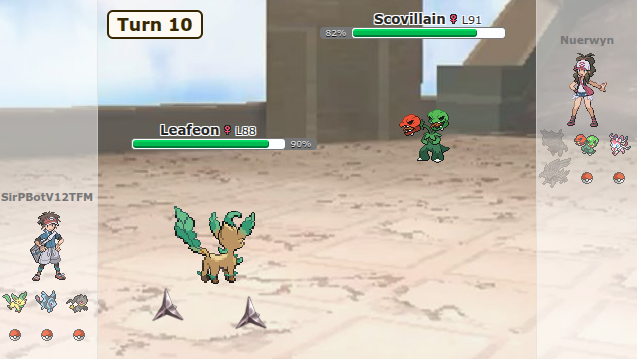
\includegraphics[width=0.88\linewidth]{images/diagrams/battle_pkmn_shwd.png}
    \caption{Captura de la interfície de Pokémon Showdown durant un combat, on s'observen els Pokémon actius de cada bàndol, les banquetes de substituts (actius, debilitats o ocults), els nivells, percentatges de vida (HP) i la informació visible de la batalla.}
    \label{fig:pokemon_showdown_battle}
\end{figure}

\subsection{De l'espècie a les estadístiques finals}
\label{subsec:stats}

Cada Pokémon pertany a una espècie concreta amb atributs únics i disposa de sis estadístiques de combat: punts de salut (\textit{Hit Points}, HP), atac, defensa, atac especial, defensa especial i velocitat~\cite{bulbapedia_pokemon,bulbapedia_stats}. Els HP determinen quant dany pot rebre; atac i defensa intervenen en els moviments físics; atac especial i defensa especial, en els moviments especials; i la velocitat decideix quin Pokémon actua abans.

La xifra final que mostra el joc es construeix a partir de cinc components:
\begin{enumerate}
    \item \textbf{Estadística base ($B$).} Pròpia de l'espècie. Dos Pikachu comparteixen les mateixes estadístiques base, però no necessàriament les mateixes xifres finals.
    \item \textbf{Nivell ($L$).} Escala el valor final. Random Battle utilitza el nivell com a mecanisme d'equilibri entre espècies.
    \item \textbf{Valors individuals (IV).} Cada estadística té un IV enter entre 0 i 31~\cite{bulbapedia_iv}.
    \item \textbf{Punts d'esforç (EV).} Es poden distribuir fins a 510 EV en total, amb un màxim efectiu de 252 en una mateixa estadística~\cite{bulbapedia_ev}.
    \item \textbf{Naturalesa ($N$).} La majoria de naturaleses multipliquen una estadística per 1,1 i una altra per 0,9~\cite{bulbapedia_nature}.
\end{enumerate}

Per a qualsevol estadística de combat diferent dels HP (Atac, Defensa, Atac Especial, Defensa Especial i Velocitat), la fórmula general d'escalat és:

\vspace{16pt}
{\large
    \begin{equation}
        \mathrm{Stat} =
        \left\lfloor
        \left(
        \left\lfloor
        \frac{(2B+\mathrm{IV}+\lfloor \mathrm{EV}/4\rfloor)L}{100}
        \right\rfloor + 5
        \right)N
        \right\rfloor .
        \label{eq:stat_formula}
    \end{equation}
}
\vspace{16pt}

Per contra, els punts de salut (HP) segueixen un càlcul diferent per dues raons mecàniques: en primer lloc, cap naturalesa modifica els HP (no s'aplica el multiplicador $N$); en segon lloc, s'afegeix el terme $+L + 10$ en comptes de la constant fixa $+5$ per tal que la salut màxima escali de manera proporcional al nivell $L$ de la criatura. Excepte casos especials com Shedinja (els HP del qual estan fixats permanentment pel motor de joc en $1$ HP independentment del nivell, IVs o EVs), la fórmula de càlcul dels HP és:

\vspace{16pt}
{\large
    \begin{equation}
        \mathrm{HP} =
        \left\lfloor
        \frac{(2B+\mathrm{IV}+\lfloor \mathrm{EV}/4\rfloor)L}{100}
        \right\rfloor + L + 10 .
        \label{eq:hp_formula}
    \end{equation}
}
\vspace{16pt}
\begin{table}[htbp]
\centering
\caption{Exemple numèric de la fórmula~\eqref{eq:stat_formula}--\eqref{eq:hp_formula} per a Pikachu a nivell 100. Les bases són les de l'espècie~\cite{bulbapedia_stats}; IV, EV i naturalesa Timid (velocitat $\times 1{,}1$, atac $\times 0{,}9$) són una configuració il·lustrativa, no un set de Random Battle.}
\label{tab:pikachu_stat_example}
\small
\begin{tabular}{lrrrrr}
\toprule
\textbf{Estadística} & \textbf{Base $B$} & \textbf{IV} & \textbf{EV} & \textbf{$N$} & \textbf{Valor final} \\
\midrule
HP & 35 & 31 & 0 & --- & 211 \\
Atac & 55 & 31 & 0 & $0{,}9$ & 131 \\
Defensa & 40 & 31 & 0 & $1{,}0$ & 116 \\
Atac especial & 50 & 31 & 0 & $1{,}0$ & 136 \\
Defensa especial & 50 & 31 & 0 & $1{,}0$ & 136 \\
Velocitat & 90 & 31 & 252 & $1{,}1$ & 306 \\
\bottomrule
\end{tabular}
\end{table}

\vspace{12pt}

Com s'observa a la Taula~\ref{tab:pikachu_stat_example}, les xifres finals calculades determinen el perfil competitiu real de la criatura durant el combat. Aquestes estadístiques finals ---especialment la Velocitat efectiva ($306$) i la salut màxima ($\mathrm{HP}=211$)--- són els valors concrets que el motor de Pokémon Showdown utilitza a cada torn per determinar l'ordre d'actuació i l'abast del dany produït. Conseqüentment, aquests valors constitueixen la base d'informació sobre la qual els agents d'IA estimen la velocitat relativa, el dany sota tirada i el risc de debilitament.

\subsection{Tipus elementals, matriu d'efectivitat i categories de moviment}
\label{subsec:tipus}

Un dels pilars estratègics del combat Pokémon és la relació elemental entre els 18 tipus existents (Foc, Aigua, Planta, etc.). Cal distingir clarament entre el \textbf{tipus del Pokémon} i el \textbf{tipus del moviment}:
\begin{itemize}
    \item \textbf{Tipus del Pokémon (funció defensiva):} Cada criatura disposa d'un o dos tipus elementals pròpis (tipus únic o \textbf{doble tipus}) que determinen les febleses, resistències i immunitats quan \emph{rep} un atac rival.
    \item \textbf{Tipus del moviment (funció ofensiva):} Atribut propi de l'acció executada. Un Pokémon no està restringit a utilitzar atacs del seu mateix tipus elemental (p. ex., un Pokémon de Foc pot llançar un atac de Terra). Tanmateix, quan el tipus del moviment coincideix amb un dels seus tipus pròpis, el joc atorga una bonificació extra del $+50\%$ al dany denominada \textbf{STAB} (\emph{Same Type Attack Bonus}, multiplicador $\times 1{,}5$).
\end{itemize}

Quan un Pokémon té \textbf{doble tipus}, els multiplicadors de la matriu d'efectivitat (Taula~\ref{tab:type_chart}) es combinen multiplicativament ($M = M_1 \times M_2$), generant efectes de \textbf{debilitat doble} ($\times 4$, p. ex., Roca contra Foc/Volador: $2 \times 2 = 4$), \textbf{resistència doble} ($\times 0{,}25$, p. ex., Planta contra Acer/Volador), \textbf{neutralització} ($\times 1$, p. ex., Lluita contra Insecte/Roca: $2 \times 0{,}5 = 1$) o \textbf{immunitat absoluta} ($\times 0$, p. ex., Elèctric contra Aigua/Terra: $2 \times 0 = 0$).

Els moviments es classifiquen en tres categories principals:
\begin{enumerate}
    \item \textbf{Físics (Atac vs. Defensa):} Atacs de contacte físic o força directa.
    \item \textbf{Especials (Atac Esp. vs. Def. Esp.):} Atacs d'energia, distància o projectils elementals.
    \item \textbf{D'estat / Suport:} No causen dany directe; s'utilitzen per induir \textbf{condicions d'estat primàries} (com cremada, paràlisi o verí; vegeu Secció~\ref{subsec:status}), modificar estadístiques, alterar el clima o col·locar perills d'entrada com \emph{Stealth Rock}.
\end{enumerate}

La diferenciació entre la via física i especial és crucial: la majoria de Pokémon s'especialitzen en un perfil defensiu físic o especial concret, la qual cosa obliga els agents d'IA a avaluar la categoria d'atac que exploti la feblesa estructural del rival.

% Taula de Tipus de Pokémon — Matriu 18×18 de multiplicadors de dany
% Fila = Tipus de l'atac, Columna = Tipus del defensor
% Requereix: \usepackage[table]{xcolor}, \usepackage{booktabs}, \usepackage{textcomp}

% Definició de colors per tipus
\definecolor{typNormal}{HTML}{A8A878}
\definecolor{typFoc}{HTML}{F08030}
\definecolor{typAigua}{HTML}{6890F0}
\definecolor{typPlanta}{HTML}{78C850}
\definecolor{typElectric}{HTML}{F8D030}
\definecolor{typGel}{HTML}{98D8D8}
\definecolor{typLluita}{HTML}{C03028}
\definecolor{typVeri}{HTML}{A040A0}
\definecolor{typTerra}{HTML}{E0C068}
\definecolor{typVolador}{HTML}{A890F0}
\definecolor{typPsiquic}{HTML}{F85888}
\definecolor{typInsecte}{HTML}{A8B820}
\definecolor{typRoca}{HTML}{B8A038}
\definecolor{typFantasma}{HTML}{705898}
\definecolor{typDrac}{HTML}{7038F8}
\definecolor{typFosc}{HTML}{705848}
\definecolor{typAcer}{HTML}{B8B8D0}
\definecolor{typFada}{HTML}{EE99AC}

% Comandes per cel·les d'efectivitat
\newcommand{\SE}{\cellcolor{green!40}\textbf{2}}
\newcommand{\NV}{\cellcolor{red!20}{\textonehalf}}
\newcommand{\IM}{\cellcolor{gray!70}\textcolor{white}{\textbf{0}}}
\newcommand{\NE}{}

% Comanda per capçaleres de tipus amb color
\newcommand{\ty}[2]{\cellcolor{#1}\textcolor{white}{\textbf{#2}}}

\begin{table}[H]
\centering
\caption{Matriu de la Taula de Tipus (Gen.\ VI--IX). Files = tipus de l'atac, columnes = tipus del defensor. \colorbox{green!40}{\scriptsize\textbf{2}} = Super Effective ($\times 2$), \colorbox{red!20}{\scriptsize\textonehalf} = Not Very Effective ($\times 0.5$), \colorbox{gray!70}{\scriptsize\textcolor{white}{\textbf{0}}} = Immunitat ($\times 0$), buit = Neutral ($\times 1$).}
\label{tab:type_chart}
\vspace{2pt}
\begin{adjustbox}{max width=\textwidth}
\tiny
\setlength{\tabcolsep}{2.5pt}
\renewcommand{\arraystretch}{1.2}
\begin{tabular}{>{\bfseries}l|c|c|c|c|c|c|c|c|c|c|c|c|c|c|c|c|c|c|}
\cline{2-19}
& \ty{typNormal}{NOR} & \ty{typFoc}{FOC} & \ty{typAigua}{AIG} & \ty{typPlanta}{PLA} & \ty{typElectric}{ELE} & \ty{typGel}{GEL} & \ty{typLluita}{LLU} & \ty{typVeri}{VER} & \ty{typTerra}{TER} & \ty{typVolador}{VOL} & \ty{typPsiquic}{PSI} & \ty{typInsecte}{INS} & \ty{typRoca}{ROC} & \ty{typFantasma}{FAN} & \ty{typDrac}{DRA} & \ty{typFosc}{FOS} & \ty{typAcer}{ACE} & \ty{typFada}{FAD} \\
\hline
\ty{typNormal}{NOR}   & \NE & \NE & \NE & \NE & \NE & \NE & \NE & \NE & \NE & \NE & \NE & \NE & \NV & \IM & \NE & \NE & \NV & \NE \\ \hline
\ty{typFoc}{FOC}      & \NE & \NV & \NV & \SE & \NE & \SE & \NE & \NE & \NE & \NE & \NE & \SE & \NV & \NE & \NV & \NE & \SE & \NE \\ \hline
\ty{typAigua}{AIG}    & \NE & \SE & \NV & \NV & \NE & \NE & \NE & \NE & \SE & \NE & \NE & \NE & \SE & \NE & \NV & \NE & \NE & \NE \\ \hline
\ty{typPlanta}{PLA}   & \NE & \NV & \SE & \NV & \NE & \NE & \NE & \NV & \SE & \NV & \NE & \NV & \SE & \NE & \NV & \NE & \NV & \NE \\ \hline
\ty{typElectric}{ELE} & \NE & \NE & \SE & \NV & \NV & \NE & \NE & \NE & \IM & \SE & \NE & \NE & \NE & \NE & \NV & \NE & \NE & \NE \\ \hline
\ty{typGel}{GEL}      & \NE & \NV & \NV & \SE & \NE & \NV & \NE & \NE & \SE & \SE & \NE & \NE & \NE & \NE & \SE & \NE & \NV & \NE \\ \hline
\ty{typLluita}{LLU}   & \SE & \NE & \NE & \NE & \NE & \SE & \NE & \NV & \NE & \NV & \NV & \NV & \SE & \IM & \NE & \SE & \SE & \NV \\ \hline
\ty{typVeri}{VER}     & \NE & \NE & \NE & \SE & \NE & \NE & \NE & \NV & \NV & \NE & \NE & \NE & \NV & \NV & \NE & \NE & \IM & \SE \\ \hline
\ty{typTerra}{TER}    & \NE & \SE & \NE & \NV & \SE & \NE & \NE & \SE & \NE & \IM & \NE & \NV & \SE & \NE & \NE & \NE & \SE & \NE \\ \hline
\ty{typVolador}{VOL}  & \NE & \NE & \NE & \SE & \NV & \NE & \SE & \NE & \NE & \NE & \NE & \SE & \NV & \NE & \NE & \NE & \NV & \NE \\ \hline
\ty{typPsiquic}{PSI}  & \NE & \NE & \NE & \NE & \NE & \NE & \SE & \SE & \NE & \NE & \NV & \NE & \NE & \NE & \NE & \IM & \NV & \NE \\ \hline
\ty{typInsecte}{INS}  & \NE & \NV & \NE & \SE & \NE & \NE & \NV & \NV & \NE & \NV & \SE & \NE & \NE & \NV & \NE & \SE & \NV & \NV \\ \hline
\ty{typRoca}{ROC}     & \NE & \SE & \NE & \NE & \NE & \SE & \NV & \NE & \NV & \SE & \NE & \SE & \NE & \NE & \NE & \NE & \NV & \NE \\ \hline
\ty{typFantasma}{FAN} & \IM & \NE & \NE & \NE & \NE & \NE & \NE & \NE & \NE & \NE & \SE & \NE & \NE & \SE & \NE & \NV & \NE & \NE \\ \hline
\ty{typDrac}{DRA}     & \NE & \NE & \NE & \NE & \NE & \NE & \NE & \NE & \NE & \NE & \NE & \NE & \NE & \NE & \SE & \NE & \NV & \IM \\ \hline
\ty{typFosc}{FOS}     & \NE & \NE & \NE & \NE & \NE & \NE & \NV & \NE & \NE & \NE & \SE & \NE & \NE & \SE & \NE & \NV & \NE & \NV \\ \hline
\ty{typAcer}{ACE}     & \NE & \NV & \NV & \NE & \NV & \SE & \NE & \NE & \NE & \NE & \NE & \NE & \SE & \NE & \NE & \NE & \NV & \SE \\ \hline
\ty{typFada}{FAD}     & \NE & \NV & \NE & \NE & \NE & \NE & \SE & \NV & \NE & \NE & \NE & \NE & \NE & \NE & \SE & \SE & \NV & \NE \\ \hline
\end{tabular}
\end{adjustbox}
\end{table}


\subsection{Teracristal·lització (Generació~IX)}
\label{subsec:teracristallitzacio}

La \textbf{Teracristal·lització} (\emph{Terastallization} o \emph{Tera}) és la mecànica transformativa exclusiva de la novena generació (\emph{Pokémon Scarlet \& Violet}, 2022) utilitzada en el format \texttt{gen9randombattle}~\cite{bulbapedia_terastal}. Aquesta mecànica permet a cada jugador transformar un dels seus Pokémon una sola vegada per combat, canviant els seus tipus elementals originals per un únic \textbf{Tipus Tera} (\emph{Tera Type}) seleccionat d'entre els 18 tipus de la matriu d'efectivitat (Taula~\ref{tab:type_chart}).

La Teracristal·lització altera la dinàmica del combat a dos nivells clau:
\begin{itemize}
    \item \textbf{Nivell defensiu:} El Pokémon adopta immediatament el Tipus Tera com a únic tipus defensiu actiu, substituint completament les seves febleses i resistències d'origen. Per exemple, un Pokémon de tipus Aigua/Volador que teracristal·litza a tipus Planta passa a ser defensivament de tipus Planta pur, convertint una feblesa fatal de $4\times$ a l'Electricitat en una resistència del $0{,}5\times$.
    \item \textbf{Nivell ofensiu (STAB millorat):} Els atacs del nou Tipus Tera obtenen la bonificació de STAB ($1{,}5\times$). Tanmateix, si el Tipus Tera coincideix amb un dels tipus originals de la criatura (p. ex., un Pokémon de Foc teracristal·litzant a Foc), la bonificació de STAB s'amplifica fins al \textbf{$2{,}0\times$} ($+100\%$ de dany). A més, el Pokémon conserva la bonificació de STAB $1{,}5\times$ en els atacs dels seus tipus primaris d'origen.
\end{itemize}

Des de la perspectiva de la presa de decisions en IA, la Teracristal·lització és un recurs d'ús únic d'alta rellevància estratègica. Permet realitzar accions de canvi de tipus instantani (\emph{type-shift}) per sobreviure a atacs directes, anular un atac supereficaç del rival i capgirar l'estat del combat en un únic torn, constituint un dels punts d'avaluació més complexos per a les polítiques de decisió dels agents.

\subsection{Velocitat, prioritat i l'empat de velocitat}
\label{subsec:velocitat}

La \textbf{Velocitat} és una de les estadístiques més determinants en el combat Pokémon competitiu. Atacar primer no només concedeix la iniciativa tàctica (\emph{tempo}), sinó que atorga la capacitat de debilitar la criatura rival abans que aquesta pugui executar la seva acció en aquell torn, anul·lant per complet el seu potencial de dany. Conseqüentment, saber quin Pokémon actuarà abans és un càlcul fonamental per als agents d'IA en avaluar els riscos i les oportunitats de cada moviment.

En cada torn, el motor de joc ordena l'execució de les accions seguint dos criteris seqüencials:

\begin{enumerate}
    \item \textbf{Prioritat del moviment:} Cada moviment té un valor de prioritat discret que varia entre $+5$ i $-7$. Els moviments de prioritat alta, com \emph{Protect} ($+4$), \emph{Extreme Speed} ($+2$) o \emph{Quick Attack} ($+1$), s'executen sempre abans que qualsevol moviment de prioritat neutra ($0$), independentment de la Velocitat dels Pokémon. Per contra, moviments d'alta utilitat tàctica com \emph{Trick Room} ($-7$) s'executen al final del torn.
    \item \textbf{Velocitat efectiva:} Si dos moviments tenen la mateixa prioritat (habitualment $0$), actua primer el Pokémon que tingui una Velocitat efectiva més alta en aquell torn, tenint en compte l'estadística final, els canvis d'etapa (de $-6$ a $+6$), els objectes equipats (com \emph{Choice Scarf}, que augmenta la velocitat en un $50\%$) i les condicions d'estat (la paràlisi redueix la velocitat a la meitat).
\end{enumerate}

Quan dos Pokémon tenen exactament la mateixa prioritat i la mateixa Velocitat efectiva final, es produeix un \textbf{empat de velocitat} (\emph{Speed Tie}). El motor de joc resol aquest empat mitjançant una decisió aleatòria al $50\%$ ($p=0{,}5$).

\subsection{Condicions d'estat primàries}
\label{subsec:status}

Com s'ha introduït en les categories de moviment (Secció~\ref{subsec:tipus}), els moviments d'estat o suport (com \emph{Will-O-Wisp} o \emph{Thunder Wave}) i certs efectes secundaris d'atacs físics o especials tenen la capacitat d'imposar \textbf{condicions d'estat primàries}. Aquestes alteracions són persistents i afecten negativament les capacitats operatives d'un Pokémon. Un Pokémon només pot patir una condició d'estat primària de manera simultània. A la Taula~\ref{tab:status} es resumeixen les principals condicions d'estat i els seus efectes mecànics en el combat.

\begin{table}[htbp]
    \centering
    \small
    \caption{Condicions d'estat primàries principals i els seus efectes mecànics en el combat Pokémon.}
    \label{tab:status}
    \vspace{2pt}
    \begin{tabular}{llp{7.5cm}}
        \toprule
        \textbf{Estat} & \textbf{Efecte en combat}               & \textbf{Mecànica i impacte tàctic}                                                                           \\ \midrule
        Cremada        & $\downarrow 50\%$ Atac físic            & Causa un dany recurrent d'1/16 dels HP màxims per torn i redueix a la meitat l'Atac físic efectiu.           \\
        Paràlisi       & $\downarrow 50\%$ Velocitat (Gen. VII+) & Redueix la Velocitat a la meitat i introdueix un $25\%$ de probabilitat de no actuar per torn.               \\
        Verí / Tòxic   & Dany recurrent per torn                 & El verí estàndard treu 1/8 dels HP per torn; el verí tòxic incrementa el dany a cada torn ($1/16, 2/16...$). \\
        Son            & Inhabilitació temporal                  & El Pokémon no pot actuar durant 1--3 torns consecutius.                                                      \\
        Congelació     & Inhabilitació estocàstica               & El Pokémon no pot actuar; té un $20\%$ de probabilitat de descongelar-se a cada torn.                        \\ \bottomrule
    \end{tabular}
\end{table}

Des de la perspectiva de la presa de decisions, induir una condició d'estat pot ser estratègicament superior a causar dany immediat. Per exemple, cremar un atacant físic enreda irreversiblement el seu potencial ofensiu, mentre que paralitzar un Pokémon ràpid permet a l'agent recuperar la iniciativa de velocitat en el combat.

\subsection{Fonts d'estocasticitat irreductibles}
\label{subsec:estocasticitat}

El combat Pokémon és un entorn fortament estocàstic. Fins i tot quan un agent disposa d'informació completa sobre l'estat actiu, el resultat d'una decisió està subjecte a tres fonts d'aleatorietat irreductibles administrades pel simulador de joc~\cite{smogon_damage,smogon_metagame,bulbapedia_stats}:

\begin{enumerate}
    \item \textbf{Tirada de dany (\emph{Damage Roll}):} El dany calculat per les fórmules oficials no és un valor fix, sinó que es multiplica per un factor aleatori extret d'una distribució uniforme discreta de 16 valors entre $0{,}85$ i $1{,}00$ ($\{0{,}85, 0{,}86, \dots, 1{,}00\}$)~\cite{smogon_damage}. Així, un mateix atac pot debilitar un rival si es dona una tirada alta ($1{,}00$), però deixar-lo amb vida si la tirada és baixa ($0{,}85$).
    \item \textbf{Precisió i evasió (\emph{Accuracy}):} Molts moviments potents no tenen una precisió del $100\%$ (p. ex., \emph{Hydro Pump} amb $80\%$ o \emph{Focus Blast} amb $70\%$)~\cite{bulbapedia_stats}. L'agent ha de ponderar el dany esperat davant del risc de fallar l'atac i regalar un torn d'iniciativa al rival.
    \item \textbf{Cop crític (\emph{Critical Hit}):} A la Generació~IX, la probabilitat base que un atac sigui crític és d'1 de cada 24 vegades ($p_{\mathrm{crit}} \approx 4{,}17\%$)~\cite{bulbapedia_stats,smogon_damage}. Un cop crític aplica un multiplicador de $\times 1{,}5$ al dany, ignora els augments defensius del rival i ignora les reduccions d'atac de l'usuari.
\end{enumerate}

Matemàticament, aquestes tres fonts d'estocasticitat es poden unificar en la formulació general del dany realitzat per un atac ofensiu:
\begin{equation}
    \mathrm{Dany} = I_{\mathrm{hit}} \cdot \left\lfloor D_{\mathrm{base}} \cdot C_{\mathrm{crit}} \cdot R \right\rfloor
    \label{eq:stochastic_damage}
\end{equation}
on $D_{\mathrm{base}}$ és el dany determinista brut derivat de les estadístiques, potència del moviment, modificadors d'etapa i la matriu de tipus (Equació~\ref{eq:stat_formula} i Secció~\ref{subsec:tipus}), mentre que els tres components estocàstics es defineixen com:
\begin{itemize}
    \item $I_{\mathrm{hit}} \sim \mathrm{Bernoulli}(P_{\mathrm{acc}})$ és l'indicador binari d'impacte, on $P_{\mathrm{acc}} \in (0, 1]$ representa la precisió efectiva de l'atac. Si l'atac falla ($I_{\mathrm{hit}}=0$), el dany resulta immediatament $0$.
    \item $C_{\mathrm{crit}}$ és la variable aleatòria del multiplicador de cop crític:
          \begin{equation}
              C_{\mathrm{crit}} = \begin{cases}
                  1{,}5 & \text{amb probabilitat } p_{\mathrm{crit}} = \frac{1}{24} \approx 4{,}17\% \quad (\text{Gen.~IX}) \\
                  1{,}0 & \text{amb probabilitat } 1 - p_{\mathrm{crit}}
              \end{cases}
          \end{equation}
          el qual, a més d'amplificar el dany, anul·la els modificadors estatístics desfavorables per a l'atacant.
    \item $R \sim \mathcal{U}(\{0{,}85, 0{,}86, \dots, 1{,}00\})$ és la tirada de dany extreta d'una distribució uniforme discreta de 16 valors, amb un valor esperat $\mathbb{E}[R] = 0{,}925$.
\end{itemize}

Així, l'esperança matemàtica del dany $\mathbb{E}[\mathrm{Dany}]$ que un agent d'IA ha d'avaluar abans de seleccionar una acció ve donada per:
\begin{equation}
    \mathbb{E}[\mathrm{Dany}] = P_{\mathrm{acc}} \cdot \mathbb{E}[R] \cdot \left( (1 - p_{\mathrm{crit}}) \cdot D_{\mathrm{norm}} + p_{\mathrm{crit}} \cdot D_{\mathrm{crit}} \right)
    \label{eq:expected_damage}
\end{equation}
on $D_{\mathrm{norm}}$ i $D_{\mathrm{crit}}$ corresponen al dany base calculat sense i amb l'omissió de modificadors d'etapa respectivament. Cal destacar que, mentre que l'Equació~\ref{eq:expected_damage} defineix l'esperança teòrica exacta del simulador de joc, a la pràctica els agents heurístics d'aquest treball utilitzen una aproximació determinista eficient ($\mathbb{E}[\mathrm{Dany}] \approx P_{\mathrm{acc}} \cdot D_{\mathrm{base}}$), ometent la branca de cop crític ($p_{\mathrm{crit}} \approx 4{,}17\%$) durant la puntuació instantània de moviments per optimitzar el temps de computació per torn.

Aquestes tres fonts d'estocasticitat, sumades a la generació procedural d'equips i als empats de velocitat (Secció~\ref{subsec:velocitat}), impedeixen l'existència de trajectòries de decisió deterministes i fan imprescindible quantificar la incertesa mitjançant simulacions estocàstiques (com l'MCTS) o polítiques d'avaluació de risc~\cite{grigsby_metamon,pokemon_rl_huang}.

\subsection{Complexitat combinatòria en la configuració d'equips}
\label{subsec:complexitat_equips}

Més enllà de la presa de decisions durant el combat, la fase prèvia de selecció i configuració d'un equip Pokémon presenta una explosió combinatòria extraordinària. Per a cada un dels membres de l'equip, cal triar l'espècie, un conjunt de 4 moviments d'entre el seu repositori disponible, la distribució de 510 Punts d'Esforç (EVs), els Valors Individuals (IVs), la Naturalesa, l'Habilitat, l'Objecte equipat i el Tipus de Teracristal·lització (un dels 18 tipus possibles a la Generació~IX).

Per a un equip de sis Pokémon, s'estima que existeixen aproximadament $608.701^{218} \approx 10^{600}$ configuracions d'equips possibles~\cite{grigsby_metamon,pokemon_rl_huang}. Per posar aquesta magnitud en perspectiva, el nombre de combinacions ($10^{600}$) supera astronòmicament el nombre total d'àtoms de l'univers observable (estimat en l'ordre de $10^{80}$), així com l'espai d'estats de jocs clàssics de la IA com els escacs ($\approx 10^{47}$) o el Go ($\approx 10^{170}$).

Aquesta immensa varietat imposa un repte metodològic central en l'avaluació d'agents d'intel·ligència artificial. En formats d'equips lliures (\emph{Teambuilding} o \emph{Custom Teams}), la taxa de victòria d'un agent pot quedar fortament emmascarada per la superioritat o el desequilibri inicial de la composició de l'equip (meta-gaming), impossibilitant mesurar amb claredat si el rendiment es deu a una presa de decisions autònoma i tàctica de qualitat o a un avantatge estructural previ. Conseqüentment, per avaluar amb rigor el raonament executiu d'un agent cal desacoblar la fase de construcció d'equips de l'execució en combat.

\subsection{El format Random Battle, el simulador Showdown i poke-env}
\label{sec:format}

Per aïllar la presa de decisions executives i eliminar els biaixos de construcció d'equips, aquest treball utilitza com a marc experimental el format oficial \textbf{Random Battle} (\texttt{gen9randombattle})~\cite{smogon_random_battle}. En aquest format, el simulador assigna proceduralment a cada jugador un equip aleatori de sis Pokémon de la Generació~IX a l'inici del combat, amb configuracions competitives optimitzades extretes del repositori públic de Smogon~\cite{smogon_rb_sets} i un mecanisme de reequilibrat dinàmic de nivells ($L$) que compensa les diferències de potència entre espècies.

Aquesta generació procedural garanteix que els agents s'enfrontin de manera contínua a escenaris no vistos i variats. Mitjançant una avaluació basada en un volum significatiu de batalles, la variància associada a la generació d'equips es cancel·la estadísticament, garantint la significança dels resultats que es detallen en la metodologia (Capítol~\ref{chap:metodologia}) i en l'avaluació empírica (Capítol~\ref{chap:resultats}).

Com a introducció conceptual a l'arquitectura d'execució, les simulacions es basen en \textbf{Pokémon Showdown}~\cite{pokemon_showdown}, el simulador de codi obert en Node.js/TypeScript que implementa amb exactitud les regles oficials del joc en un entorn \emph{headless} i local, i la llibreria en Python \textit{poke-env}~\cite{poke_env} (versió 0.11.x), que exposa la interfície de comunicació per a la connexió d'agents autònoms. Aquesta breu introducció serveix de fonament teòric abans de desenvolupar en profunditat la infraestructura d'execució, el protocol de comunicació i el disseny detallat dels entorns al Capítol~\ref{chap:metodologia}.

\subsection{Síntesi del domini: Pokémon com a entorn benchmark ideal per a la IA}
\label{subsec:sintesi_domini}

En resum, el combat Pokémon en el format \texttt{gen9randombattle} configura un entorn de decisió d'una complexitat extraordinària. A diferència dels jocs tradicionals de la IA que aïllen només una o dues dificultats, Pokémon és un dels pocs dominis en la literatura que encreua simultàniament quatre reptes centrals de la intel·ligència artificial (Figura~\ref{fig:statistical_reason}):

\begin{enumerate}
    \item \textbf{Planificació a llarg termini (\emph{Long-Term Planning}):} Propi de jocs d'estratègia posicional pura com els \textbf{escacs} o el \textbf{Go}. A Pokémon, les decisions no es poden valorar aïlladament per al torn actual: cal gestionar un equip de sis criatures al llarg de desenes de torns, sacrificant Pokémon per conservar la iniciativa (\emph{tempo}), col·locant perills d'entrada (\emph{hazards}) o preparant condicionants de victòria (\emph{win conditions}) per al final del combat.
    \item \textbf{Accions simultànies (\emph{Simultaneous Actions}):} Present en jocs com el \textbf{Pedra-Paper-Tisores} o variants d'\textbf{escacs a cegues} (\emph{Kriegspiel}). A cada torn, tots dos jugadors escullen la seva acció de manera secreta i simultània (Secció~\ref{sec:pokemon_joc}). L'agent no pot simplement reaccionar a un moviment vist, sinó que ha de raonar estratègicament sobre la matriu de respostes rivals des de la teoria de jocs.
    \item \textbf{Gestió de la probabilitat i l'estocasticitat (\emph{Probability Management}):} Típic de jocs de \textbf{daus} o \textbf{Backgammon}. Les tirades de dany, la precisió dels moviments, els cops crítics (Secció~\ref{subsec:estocasticitat}) i la generació procedural d'equips (Secció~\ref{sec:format}) impedeixen l'existència de trajectòries deterministes, obligant l'agent a ponderar riscos i esperances matemàtiques a cada decisió.
    \item \textbf{Informació imperfecta i oculta (\emph{Imperfect Information}):} Propi de jocs de cartes com el \textbf{Pòquer} o \textbf{\textit{Magic: The Gathering}}. L'estat inicial del rival (moviments no revelats, objectes, habilitats, IVs/EVs i Tipus Tera) roman ocult fins que s'exposa en combat, exigint a l'agent mantenir i actualitzar una distribució de creença sobre les variables no observades.
\end{enumerate}

La convergència d'aquests quatre eixos (esquematitzada a la Figura~\ref{fig:statistical_reason}) converteix el combat Pokémon en un entorn benchmark d'un interès excepcional per a la intel·ligència artificial. Cap d'aquests quatre reptes es pot abordar de manera aïllada, ja que la presa de decisions exigeix ponderar simultàniament la planificació temporal a llarg termini, l'estocasticitat del motor i la incertesa sobre les accions i l'estat del rival.

\begin{figure}[htbp]
    \centering
    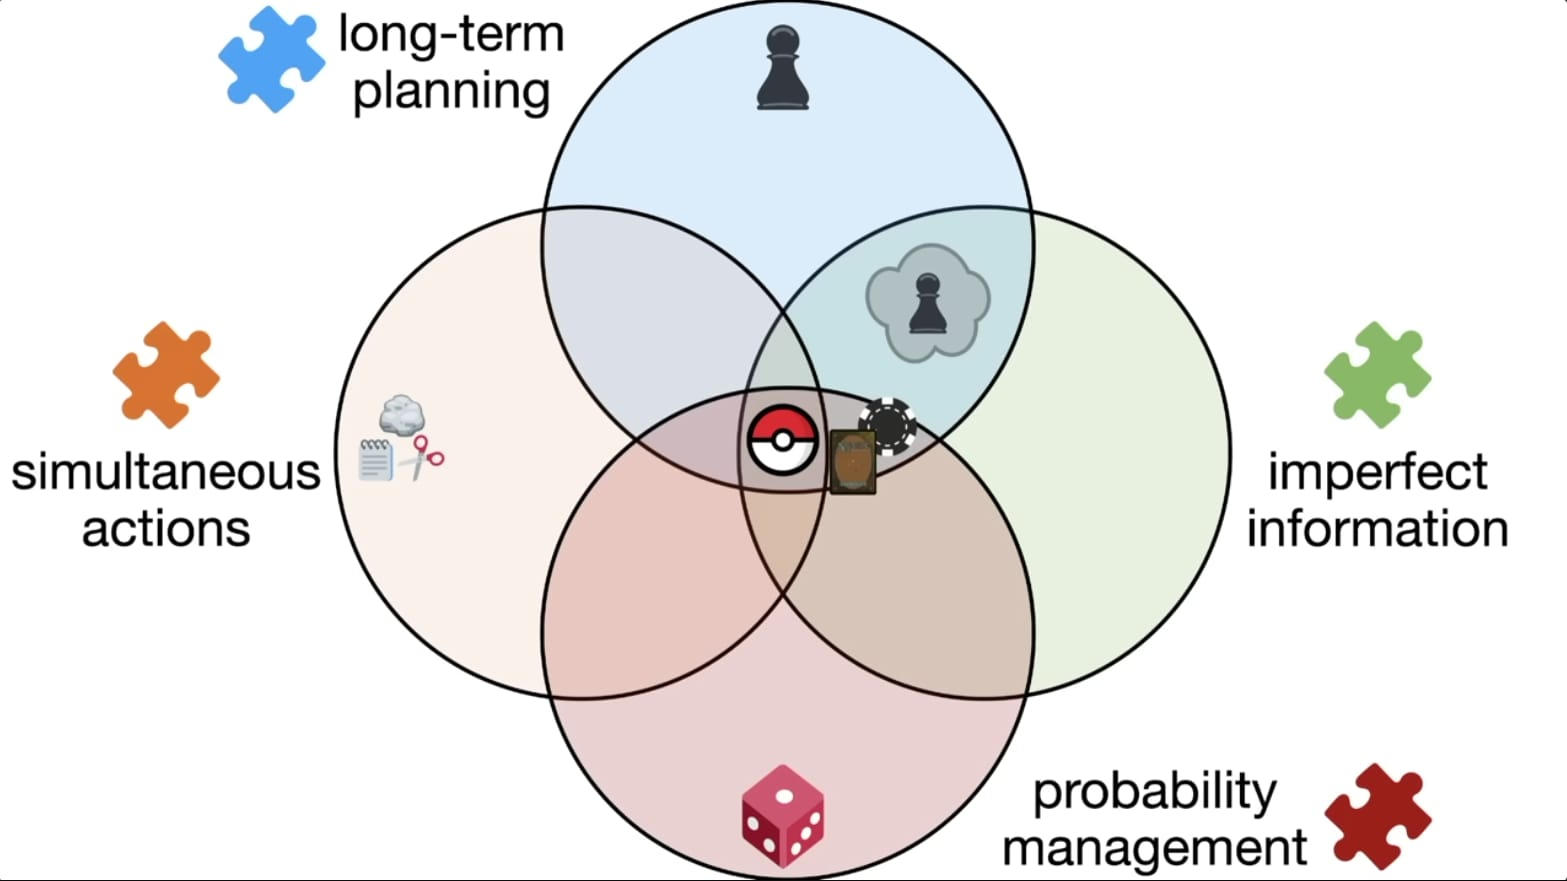
\includegraphics[width=0.75\linewidth]{images/diagrams/stadistical_reason.jpeg}
    \caption{Intersecció dels quatre eixos fonamentals de complexitat en IA i la seva correspondència amb altres jocs.}
    \label{fig:statistical_reason}
\end{figure}

Aquesta combinació única de propietats fa imprescindible formalitzar el problema des de la teoria de jocs i el marc dels processos de decisió sota incertesa. En la secció següent (Secció~\ref{sec:ia_jocs}), es tradueixen aquestes mecàniques al modelat matemàtic rigorós mitjançant Processos de Decisió de Markov Parcialment Observables (POMDP) i Jocs Estocàstics d'Observació Parcial (POSG).

% ============================================================
\section{Formalització matemàtica i marc d'inferència estadística}
\label{sec:ia_jocs}

Una vegada descrites les mecàniques del joc i les seves propietats estructurals (Secció~\ref{sec:pokemon_joc}), aquesta secció formalitza matemàticament el problema des de la teoria de jocs, el marc dels processos de decisió sota incertesa (POMDP i POSG) i estableix les bases d'inferència estadística utilitzades per avaluar rigorosament els agents.

\subsection{De la informació perfecta a la informació imperfecta}

Els jocs han estat el banc de proves clàssic de la IA, des dels escacs~\cite{shannon_chess,CAMPBELL200257} i el Go~\cite{alphago,alphazero} (informació perfecta) fins a videojocs d'estratègia i entorns amb informació amagada com StarCraft~II~\cite{alphastar}, Dota~2~\cite{openai_five} o el pòquer~\cite{libratus,pluribus} (informació imperfecta).

La distinció operativa clau és:
\begin{itemize}
    \item \textbf{Informació perfecta} (escacs, Go): l'estat complet $s$ és comú i totalment visible per a tots els jugadors a cada torn.
    \item \textbf{Informació imperfecta} (pòquer, StarCraft, Pokémon): part de l'estat roman oculta als jugadors. Cal mantenir una distribució de creença sobre les variables no observades i inferir les opcions del rival.
\end{itemize}

\subsection{Formalització dels Processos de Decisió: MDP, POMDP i POSG}

Un \textbf{Procés de Decisió de Markov (MDP)}~\cite{sutton_barto} es defineix com la tupla $(S,A,T,R,\gamma)$, on $S$ és l'espai d'estats, $A$ l'espai d'accions, $T(s'\mid s,a) = P(S_{t+1}=s'\mid S_t=s, A_t=a)$ la funció de transició estocàstica, $R(s,a)$ la funció de recompensa i $\gamma \in [0,1]$ el factor de descompte. La política $\pi(a\mid s)$ maximitza el retorn esperat.

Quan l'agent no observa directament l'estat real $s$, sinó una observació parcial $o\in\Omega$ emesa segons una funció d'emissió $O(o\mid s',a) = P(O_{t+1}=o\mid S_{t+1}=s', A_t=a)$, el model es converteix en un \textbf{Procés de Decisió de Markov Parcialment Observable (POMDP)}~\cite{pomdp,kaelbling_pomdp}.

Atès que a Pokémon hi intervenen dos jugadors que escullen accions de forma simultània sense conèixer la decisió del rival en el torn actual, el model formal conceptualment rigorós és un \textbf{Joc Estocàstic d'Observació Parcial (POSG)}~\cite{shapley_stochastic_games,von_neumann}. Formalsment, un POSG de dos jugadors es defineix com una tupla de vuit components:
\begin{equation}
    \mathcal{M} = \left( N, S, \{A_i\}_{i \in N}, T, \{R_i\}_{i \in N}, \{\Omega_i\}_{i \in N}, \{O_i\}_{i \in N}, \gamma \right)
    \label{eq:posg_tuple}
\end{equation}
on:
\begin{itemize}
    \item $N = \{1, 2\}$ és el conjunt dels dos jugadors (Jugador 1 i Jugador 2).
    \item $S$ és l'espai d'estats globals del joc.
    \item $A_i$ és l'espai d'accions del jugador $i$. Una acció conjunta s'expressa com $\mathbf{a} = (a_1, a_2) \in A_1 \times A_2$.
    \item $T(s'\mid s, \mathbf{a}) = P(S_{t+1}=s'\mid S_t=s, \mathbf{a}_t=\mathbf{a})$ és la probabilitat de transició condicional sota l'acció conjunta.
    \item $R_i(s, \mathbf{a})$ és la recompensa del jugador $i$. En ser un joc competitiu pur de suma zero, es compleix $R_1(s, \mathbf{a}) + R_2(s, \mathbf{a}) = 0$.
    \item $\Omega_i$ és l'espai d'observacions privades del jugador $i$.
    \item $O_i(o_i\mid s', \mathbf{a}) = P(O_{i,t+1}=o_i\mid S_{t+1}=s', \mathbf{a}_t=\mathbf{a})$ és la funció d'emissió d'observacions privades.
    \item $\gamma \in [0, 1]$ és el factor de descompte temporal.
\end{itemize}

\begin{figure}[htbp]
    \centering
    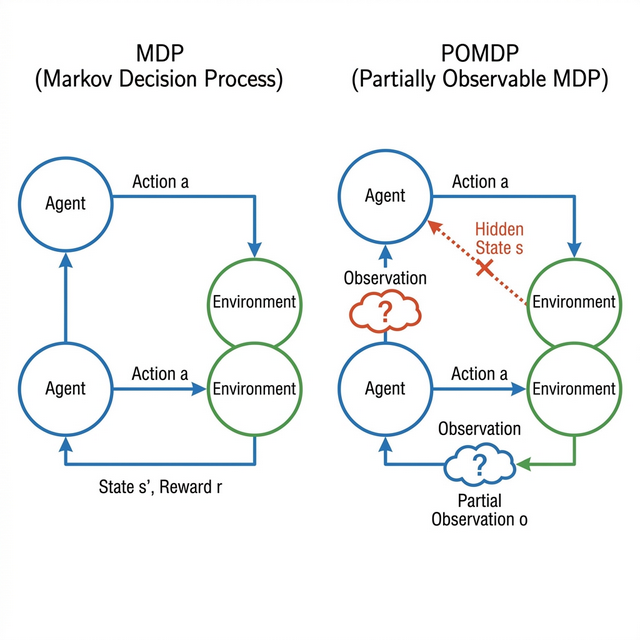
\includegraphics[width=0.72\linewidth]{images/diagrams/mdp_vs_pomdp.png}
    \caption{Diferència conceptual entre un MDP, un POMDP i un POSG. En el POMDP l'agent rep una observació parcial de l'estat. Una batalla Pokémon afegeix un segon decisor simultani i s'aproxima exactament amb un POSG.}
    \label{fig:mdp_pomdp}
\end{figure}

\subsection{Estat de creença, matriu de pagaments i reducció d'enginyeria}

A causa de la informació oculta, el jugador $i$ no pot basar la seva decisió directament en l'estat real $s$, sinó en un \textbf{estat de creença} (\emph{Belief State}) $b_{i,t}(s) \in \Delta(S)$, definit com la distribució de probabilitat sobre els possibles estats globals $s$ donada la seva història d'observacions i accions $h_{i,t} = (o_{i,1}, a_{i,1}, \dots, o_{i,t})$:
\begin{equation}
    b_{i,t}(s) = P(S_t = s \mid h_{i,t})
    \label{eq:belief_state}
\end{equation}
Aquest estat de creença s'actualitza a cada torn mitjançant la regla de Bayes al rebre la nova observació $o_{i,t+1}$.

D'altra banda, a causa de la simultaneïtat de les accions, a cada pas de decisió els dos jugadors s'enfronten a una matriu de pagaments de forma normal $M(a_1, a_2) = \mathbb{E}_{s \sim b} [R_1(s, a_1, a_2) + \gamma V(s')]$. Com que qualsevol política pura determinista $\pi_i(a_i)$ és explotable per l'oponent (p. ex., si un agent ataca de manera predictible, el rival canviarà a un Pokémon immune), les polítiques òptimes requereixen la selecció de \textbf{polítiques estocàstiques / estratègies mixtes} $\pi_1 \in \Delta(A_1)$ i $\pi_2 \in \Delta(A_2)$ per assolir un \textbf{Equilibri de Nash}:
\begin{equation}
    \mathbb{E}_{\mathbf{a} \sim (\pi_1^*, \pi_2^*)} [R_1(s, \mathbf{a})] \ge \mathbb{E}_{a_1 \sim \pi_1, a_2 \sim \pi_2^*} [R_1(s, a_1, a_2)], \qquad \forall \pi_1 \in \Delta(A_1)
    \label{eq:nash_equilibrium}
\end{equation}

Des del punt de vista computacional, resoldre un POSG general és un problema de complexitat $NEXP$-hard. Per aquest motiu, els cinc paradigmes desenvolupats en aquest treball apliquen reduccions d'enginyeria:
\begin{itemize}
    \item \textbf{Aprenentatge per Reforç (PPO) i Clonatge Conductual (XGBoost)}: Absorbeixen la política del rival $\pi_2(a_2 \mid o_2)$ dins de la funció de transició de l'entorn:
          \begin{equation}
              T_{\mathrm{eff}}(s'\mid s, a_1) = \sum_{a_2 \in A_2} \pi_2(a_2 \mid o_2) \cdot T(s'\mid s, a_1, a_2)
              \label{eq:eff_transition}
          \end{equation}
          Aquesta reducció transforma el POSG multijugador en un \textbf{POMDP de decisió individual} des de la perspectiva de l'agent.
    \item \textbf{Cerca Minimax i MCTS}: Construeixen localment la matriu de respostes o simulen *rollouts* d'esperança sobre l'arbre de decisions d'un torn o de pocs torns a l'arrel.
\end{itemize}

\subsection{Instanciació dels components a \texttt{gen9randombattle}}

A la Taula~\ref{tab:pomdp_pokemon} es detalla com es mapeja exactament cadascun dels components formals del POSG/POMDP al domini del combat individual de \texttt{gen9randombattle}.

\begin{table}[H]
    \centering
    \small
    \begin{tabular}{|l|p{10.5cm}|}
        \hline
        \textbf{Component} & \textbf{Instanciació a Singles \texttt{gen9randombattle}}                                                                                                                                    \\ \hline
        $S$                & Sis Pokémon per bàndol (espècie, HP, configuració, objecte, habilitat, modificadors i condició d'estat), clima, perills d'entrada, Tera consumit i torn. $|S|$ és astronòmic i no s'enumera. \\ \hline
        $A$                & Fins a quatre moviments, cinc canvis i la Teracristal·lització com a modificador. La legalitat depèn de PP, debilitaments i bloqueigs; el PPO ho codifica en 14 índexs.                      \\ \hline
        $T$                & Motor de Showdown: dany amb roll $[0{,}85,1{,}00]$, STAB, Taula de Tipus, prioritat, velocitat, secundaris.                                                                                  \\ \hline
        $R$                & Recompensa terminal conceptual $+1$ per victòria i $-1$ per derrota. Per a l'avaluació s'enregistra l'indicador binari $W\in\{0,1\}$ i se'n publica la mitjana.                              \\ \hline
        $\Omega$           & Equip propi complet; del rival, espècies revelades, percentatge d'HP, moviments utilitzats i condicions laterals. EV, naturalesa, objecte i moviments no revelats romanen ocults.            \\ \hline
    \end{tabular}
    \caption{Mapatge POSG/POMDP al combat individual de Random Battle (Generació~IX).}
    \label{tab:pomdp_pokemon}
\end{table}

\subsection{Marc d'avaluació estadística i mètodes d'inferència}
\label{subsec:marc_estadistic}

Per comparar de manera científicament rigorosa la capacitat de decisió dels 28 agents desenvolupats, s'estableix un marc d'inferència estadística basat en tres eines fonamentals:

\begin{enumerate}
    \item \textbf{Estimació de la Taxa de Victòria (\emph{Win Rate}):}
          En un enfrontament de $N$ partides entre dos agents, cada combat $i$ s'escriu com una variable aleatòria binària de Bernoulli $W_i \sim \mathrm{Bernoulli}(p)$, on $W_i = 1$ indica victòria de l'agent i $W_i = 0$ indica derrota. L'estimador puntual de la taxa de victòria $\hat{p}$ és la mitjana mostral:
          \begin{equation}
              \hat{p} = \frac{1}{N} \sum_{i=1}^N W_i
              \label{eq:win_rate_estimator}
          \end{equation}

    \item \textbf{Intervals de Confiança de Wilson (\emph{Wilson Score Interval}):}
          A diferència de l'interval binomi estàndard de Wald ($\hat{p} \pm z \sqrt{\hat{p}(1-\hat{p})/N}$), que falla prop dels límits ($0$ o $1$) o en mostres asimètriques, aquest treball calcula els intervals de confiança mitjançant l'\textbf{interval de la puntuació de Wilson}~\cite{wilson_1927}:
          \begin{equation}
              \mathrm{CI}_{\mathrm{Wilson}} = \frac{1}{1 + \frac{z^2}{N}} \left( \hat{p} + \frac{z^2}{2N} \pm z \sqrt{\frac{\hat{p}(1-\hat{p})}{N} + \frac{z^2}{4N^2}} \right)
              \label{eq:wilson_ci}
          \end{equation}
          on $z = z_{1-\alpha/2} = 1{,}96$ per a un nivell de confiança del $95\%$ ($\alpha = 0{,}05$).

    \item \textbf{Sistema de Puntuació Elo i Model de Bradley-Terry:}
          Per ordenar els 28 agents en un llistat global independent de parelles individuals, s'utilitza el model de comparació per parelles de Bradley-Terry / Sistema de Puntuació Elo~\cite{elo_rating,bradley_terry_1952}. La probabilitat esperada de victòria de l'agent $A$ enfront de l'agent $B$ amb puntuacions $R_A$ i $R_B$ ve donada per la funció logística:
          \begin{equation}
              E_A = \frac{1}{1 + 10^{(R_B - R_A)/400}}
              \label{eq:elo_expected}
          \end{equation}
          I l'actualització de la puntuació Elo després de cada combat amb resultat $S_A \in \{0, 1\}$ segueix:
          \begin{equation}
              R_A' = R_A + K (S_A - E_A)
              \label{eq:elo_update}
          \end{equation}
          on $K$ és el factor d'ajust d'escala.
\end{enumerate}

Finalment, la reducció de la variància de generació d'equips s'aconsegueix mitjançant un volum massiu d'avaluació ($N > 6{,}4 \times 10^6$ batalles totals), la qual cosa redueix l'error estàndard $SE = \sqrt{\frac{p(1-p)}{N}}$ per sota del $0{,}3\%$ ($SE < 0{,}003$), danyant una significança estadística del $p < 0{,}001$ en totes les comparacions presentades als Capítols~\ref{chap:metodologia} i~\ref{chap:resultats}.

% ============================================================
\section{Estat de l'Art en IA i Pokémon}
\label{sec:estat_art}

\textit{poke-env}~\cite{poke_env,pokemon_ai_sahovic} va facilitar l'ús de Pokémon Showdown com a entorn d'aprenentatge. La biblioteca inclou \texttt{RandomPlayer}, \texttt{MaxBasePowerPlayer} i \texttt{SimpleHeuristicsPlayer}.

Huang i Lee~\cite{pokemon_rl_huang} van entrenar un agent PPO amb \textit{self-play} a Showdown. Més recentment, Grigsby et al.~\cite{grigsby_metamon} van aplicar imitació i RL fora de línia amb Transformers (*Metamon*) sobre repeticions humanes. \textit{PokéChamp}~\cite{pokechamp,pokechamp_icml} combina un model de llenguatge (LLM) amb cerca minimax d'un pas i va assolir el Top 3 d'Elo al ladder públic de Showdown. \textit{PokéLLMon}~\cite{pokellmon} utilitza així mateix models de llenguatge per a la presa de decisions en combat.

\subsection{Què afegeix aquest TFM}

\begin{enumerate}
    \item \textbf{Una matriu comuna de 28 agents} per a heurístiques, minimax, MCTS ras i imitació, amb oponents compartits, volums mostrals explícits ($>6{,}4$M de batalles) i telemetria per decisió.
    \item \textbf{Una seqüència de catorze heurístiques} (\texttt{v1}--\texttt{v14}) que permet estudiar ablacions de coneixement de domini.
    \item \textbf{Variants guiades i no guiades} de cerca i d'imitació, amb \texttt{v14} com a prior o executor.
    \item \textbf{Una avaluació rigorosa de MaskablePPO} contra \texttt{v12}, amb inicialització per clonatge conductual.
\end{enumerate}

% ============================================================
\section{Fonaments teòrics dels cinc paradigmes de decisió}
\label{sec:ia_tecniques}

Cada paradigma introdueix un mecanisme diferent: coneixement codificat, anticipació adversària, simulació, supervisió amb dades humanes o optimització per reforç.

\begin{table}[htbp]
\centering
\caption{Comparació conceptual dels cinc paradigmes. Tots decideixen sobre el mateix simulador i format; canvia la font de coneixement i el còmput per torn.}
\label{tab:paradigm_mechanisms}
\small
\renewcommand{\arraystretch}{1.3}
\begin{tabularx}{\textwidth}{l>{\raggedright\arraybackslash}X>{\raggedright\arraybackslash}X>{\raggedright\arraybackslash}X>{\raggedright\arraybackslash}p{2.2cm}}
\toprule
\textbf{Paradigma} & \textbf{Què decideix} & \textbf{Coneixement} & \textbf{Còmput per torn} & \textbf{Aprèn?} \\
\midrule
Heurística & Argmax d'una puntuació fixa sobre accions legals. & Regles escrites (dany, posició, Tera). & Constant, baix. & No durant l'execució. \\
\arrayrulecolor{gray!30}\hline\arrayrulecolor{black}
Minimax d'un torn & Maximin sobre una matriu d'accions i respostes estimades. & Funció de fulla + prior opcional. & Enumeració d'un torn. & No. \\
\arrayrulecolor{gray!30}\hline\arrayrulecolor{black}
MCTS ras & UCB/PUCT només als fills de l'arrel. & Determinització i, a \texttt{v20}, prior de \texttt{v14}. & 100 simulacions de 5 torns. & No (cerca en línia). \\
\arrayrulecolor{gray!30}\hline\arrayrulecolor{black}
Imitació & Classificador atacar/canviar + executor. & Trajectòries humanes Elo~$1800+$. & Inferència XGBoost. & Supervisat, fora de línia. \\
\arrayrulecolor{gray!30}\hline\arrayrulecolor{black}
PPO & Política estocàstica emmascarada $\pi_\theta(a\mid o)$. & Interacció amb recompensa + clonatge inicial. & Un pas de xarxa. & Per reforç, fora de partida. \\
\bottomrule
\end{tabularx}
\end{table}


\subsection{Heurístiques: coneixement com a ablació}

Una heurística no ajusta els seus paràmetres durant l'execució. A cada decisió puntua les accions legals amb regles fixes i tria l'argmax. La seqüència \texttt{v1}--\texttt{v14} funciona com una \textbf{ablació incremental}: permet relacionar blocs de coneixement amb canvis de rendiment.

\subsection{Minimax d'un torn: resposta adversària immediata}

Minimax~\cite{minimax_knuth} assigna a cada estat el valor de la millor acció sota la resposta més desfavorable. Com que a Pokémon les accions del torn són simultànies, la implementació construeix una matriu d'accions pròpies i respostes rivals estimades (\texttt{v15}--\texttt{v17}). La funció de fulla de \texttt{v15} és:
\begin{equation}
    V = \mathrm{HP}_{\mathrm{me}} - 1{,}5\,\mathrm{HP}_{\mathrm{opp}} + \text{bonificacions}.
\end{equation}
\texttt{v16} afegeix bonificacions posicionals i \texttt{v17} suma un prior de $+0{,}15$ a l'acció de \texttt{v14}.

\subsection{Cerca de Monte Carlo a l'arrel (shallow MCTS)}

L'MCTS complet~\cite{mcts_survey,coulom_mcts} alterna selecció, expansió, simulació i retropropagació en un arbre. La implementació d'aquest treball (\texttt{v18}--\texttt{v20}) aplica UCB1 o PUCT només als fills de l'\textbf{arrel}, executant 100 simulacions de 5 torns amb \texttt{LocalSim}~\cite{pokechamp}.

\begin{figure}[htbp]
    \centering
    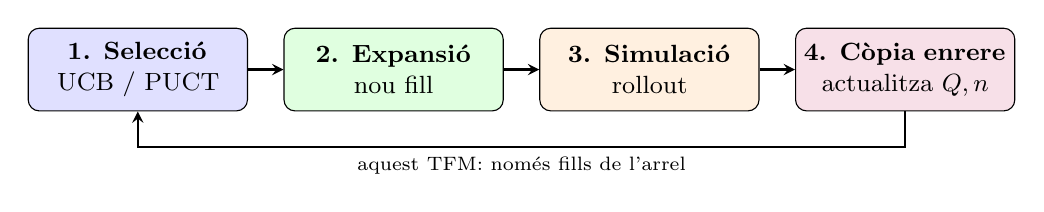
\begin{tikzpicture}[
            font=\small,
            box/.style={rectangle, rounded corners, draw, align=center, minimum height=1.05cm, text width=2.55cm},
            arr/.style={->, thick, >=stealth}
        ]
        \node[box, fill=blue!12] (sel) {\textbf{1. Selecció}\\UCB / PUCT};
        \node[box, fill=green!12, right=0.45cm of sel] (exp) {\textbf{2. Expansió}\\nou fill};
        \node[box, fill=orange!12, right=0.45cm of exp] (sim) {\textbf{3. Simulació}\\rollout};
        \node[box, fill=purple!12, right=0.45cm of sim] (back) {\textbf{4. Còpia enrere}\\actualitza $Q,n$};
        \draw[arr] (sel) -- (exp);
        \draw[arr] (exp) -- (sim);
        \draw[arr] (sim) -- (back);
        \draw[arr] (back.south) -- ++(0,-0.45) -| node[below, font=\scriptsize, pos=0.25] {aquest TFM: només fills de l'arrel} (sel.south);
    \end{tikzpicture}
    \caption{Cicle clàssic de l'MCTS adaptat a simulacions de 5 torns a l'arrel.}
    \label{fig:mcts_cycle}
\end{figure}

UCB1:
\begin{equation}
    \mathrm{UCB1}(j) = \bar X_j + C\sqrt{\frac{\ln N}{n_j}}, \qquad C=1{,}4.
\end{equation}
PUCT (\texttt{v20}) afegeix un prior $\pi(a)$ extret de \texttt{v14} amb un pes de $0{,}70$.

\subsection{Imitació / clonatge conductual}

L'aprenentatge per imitació (\textit{behavioral cloning}) premia imitar trajectòries d'experts~\cite{pomerleau_alvinn,argall_lfd}. \texttt{v21} utilitza un model XGBoost~\cite{xgboost} sobre 1,12 milions de torns d'experts (Elo~$1800+$) per a la decisió macro i delega a \texttt{v14} l'execució micro. \texttt{v22} és un model dual purament d'imitació (dos classificadors XGBoost).

\subsection{PPO amb emmascarament d'accions}

L'aprenentatge per reforç~\cite{sutton_barto} optimitza una política d'actor-crític~\cite{konda_actor_critic}. MaskablePPO~\cite{ppo,huang_action_masking,sb3_contrib} utilitza l'objectiu retallat:
\begin{equation}
    L^{\mathrm{CLIP}}(\theta)=\hat{\mathbb{E}}_t\left[\min\left(r_t(\theta)\hat A_t,\;\mathrm{clip}(r_t(\theta),1-\epsilon,1+\epsilon)\hat A_t\right)\right].
\end{equation}

\begin{figure}[htbp]
    \centering
    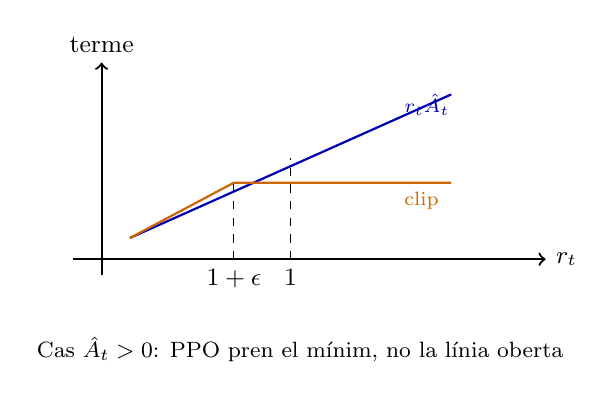
\begin{tikzpicture}[font=\small, x=2.4cm, y=1.35cm]
        \draw[->, thick] (-0.15,0) -- (2.35,0) node[right] {$r_t$};
        \draw[->, thick] (0,-0.15) -- (0,1.85) node[above] {terme};
        \draw[thick, blue!70!black] (0.15,0.2) -- (1.85,1.55);
        \draw[thick, orange!80!black] (0.15,0.2) -- (0.7,0.72) -- (1.85,0.72);
        \draw[dashed] (0.7,0) node[below] {$1+\epsilon$} -- (0.7,0.72);
        \draw[dashed] (1,0) node[below] {$1$} -- (1,0.95);
        \node[font=\scriptsize, blue!70!black, anchor=west] at (1.55,1.45) {$r_t\hat A_t$};
        \node[font=\scriptsize, orange!80!black, anchor=west] at (1.55,0.55) {clip};
        \node[font=\footnotesize] at (1.05,-0.85) {Cas $\hat A_t>0$: PPO pren el mínim, no la línia oberta};
    \end{tikzpicture}
    \caption{Intuïció de l'objectiu retallat de PPO.}
    \label{fig:ppo_clip}
\end{figure}

L'emmascarament d'accions assigna probabilitat nul·la a accions il·legals. El clonatge conductual previ inicialitza l'actor a partir de 400 partides de \texttt{v8}.

% ============================================================
\section{Síntesi del marc teòric}
\label{sec:marc_teoric_sintesi}

El marc teòric queda definit per les mecàniques del combat Pokémon individual, el format \texttt{gen9randombattle}, la formalització matemàtica POSG/POMDP i els fonaments dels cinc paradigmes d'agents. Aquestes bases permeten avaluar amb rigor experimental els resultats empírics que es presenten als capítols següents.

\chapter{Metodologia: Disseny Experimental}
\label{chap:metodologia}

Aquest capítol fixa l'entorn, la matriu, les mètriques i ---amb fórmula, no amb una cita d'una línia--- per què el gauntlet usa 10.000 partides per cel·la i 1.000 quan intervé MCTS. Sense aquest protocol, els nombres del Capítol~\ref{chap:resultats} no es poden llegir.

% ============================================================
\section{Entorn de Simulació}
\label{sec:entorn}

\subsection{Arquitectura client--servidor de Pokémon Showdown}

Showdown~\cite{pokemon_showdown} és una aplicació Node.js amb protocol WebSocket. En recerca s'executa localment:

\begin{verbatim}
  node pokemon-showdown start --port 8000 --no-security
\end{verbatim}

\texttt{--no-security} desactiva autenticació. Cada instància ocupa un port TCP i guarda l'estat de les batalles en RAM. Els missatges són text amb delimitador \texttt{|}:

\begin{verbatim}
  |move|p1a: Pikachu|Thunderbolt|p2a: Gyarados
  |-damage|p2a: Gyarados|23/100
  |-supereffective|p2a: Gyarados
  |turn|5
\end{verbatim}

El missatge crític per a l'agent és \texttt{|request|}, un JSON amb moviments legals, PP, stats \emph{pròpies} i HP. Les stats i l'objecte del rival \textbf{no} hi són: això és $\Omega\subset S$.

L'agent respon amb \texttt{/choose move 1}, \texttt{/choose switch 4} o \texttt{/choose move 1 terastallize}. El servidor resol el torn de forma atòmica (prioritat, velocitat, dany, secundaris) i emet el log.

\begin{figure}[H]
    \centering
    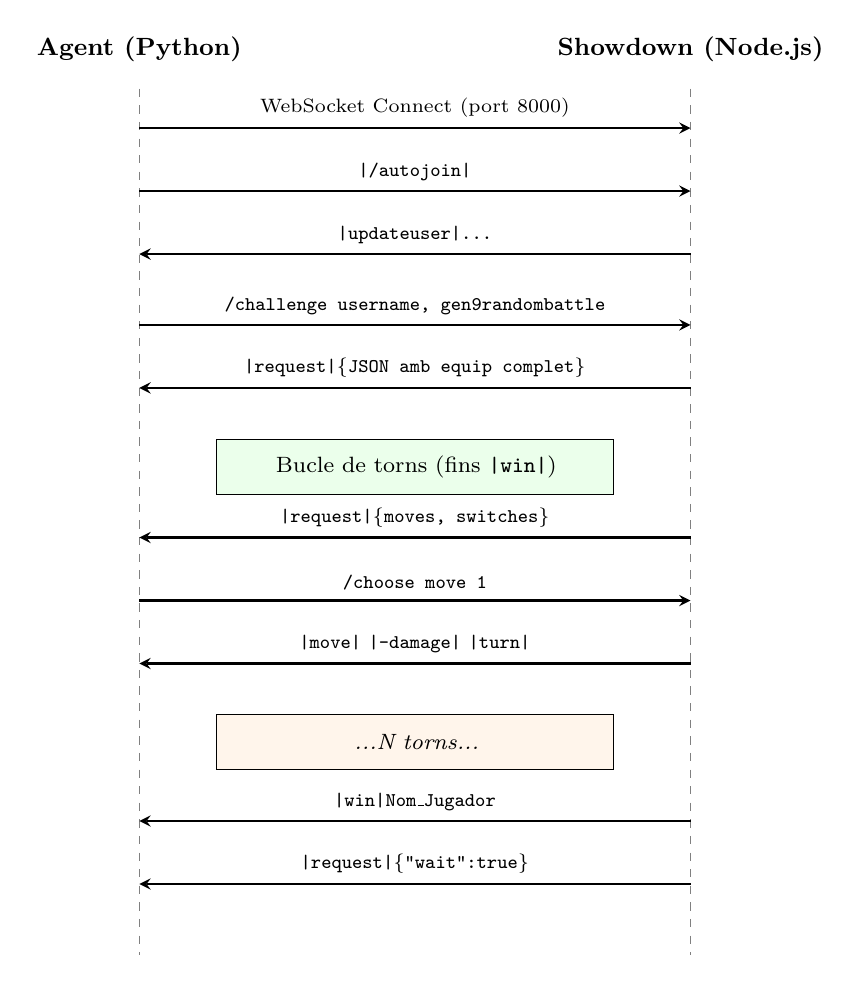
\begin{tikzpicture}[
        node distance=1.1cm, auto, font=\footnotesize,
        block/.style={rectangle, draw, fill=blue!5, text width=4.8cm, align=center, minimum height=0.7cm},
        msg/.style={->, thick, >=stealth},
        lbl/.style={font=\scriptsize, midway}
    ]
        \node[font=\small\bfseries] (agent_title) at (0,0) {Agent (Python)};
        \node[font=\small\bfseries] (server_title) at (7,0) {Showdown (Node.js)};
        \draw[dashed, gray] (0,-0.5) -- (0,-11.5);
        \draw[dashed, gray] (7,-0.5) -- (7,-11.5);

        \draw[msg] (0,-1) -- node[above, lbl]{WebSocket Connect (port 8000)} (7,-1);
        \draw[msg] (0,-1.8) -- node[above, lbl]{\texttt{|/autojoin|}} (7,-1.8);
        \draw[msg, <-] (0,-2.6) -- node[above, lbl]{\texttt{|updateuser|...}} (7,-2.6);

        \draw[msg] (0,-3.5) -- node[above, lbl]{\texttt{/challenge username, gen9randombattle}} (7,-3.5);
        \draw[msg, <-] (0,-4.3) -- node[above, lbl]{\texttt{|request|\{JSON amb equip complet\}}} (7,-4.3);

        \node[block, fill=green!8] at (3.5,-5.3) {Bucle de torns (fins \texttt{|win|})};

        \draw[msg, <-] (0,-6.2) -- node[above, lbl]{\texttt{|request|\{moves, switches\}}} (7,-6.2);
        \draw[msg] (0,-7.0) -- node[above, lbl]{\texttt{/choose move 1}} (7,-7.0);
        \draw[msg, <-] (0,-7.8) -- node[above, lbl]{\texttt{|move|} \texttt{|-damage|} \texttt{|turn|}} (7,-7.8);

        \node[block, fill=orange!8] at (3.5,-8.8) {\textit{...N torns...}};

        \draw[msg, <-] (0,-9.8) -- node[above, lbl]{\texttt{|win|Nom\_Jugador}} (7,-9.8);
        \draw[msg, <-] (0,-10.6) -- node[above, lbl]{\texttt{|request|\{"wait":true\}}} (7,-10.6);
    \end{tikzpicture}
    \caption{Protocol WebSocket d'una batalla local. L'estat viu a la RAM del procés Node.js; el servidor és determinista donats inputs i llavor RNG.}
    \label{fig:cicle_batalla}
\end{figure}

Latència típica d'un torn heurístic en local: $<5$~ms. MCTS, amb 100 \texttt{LocalSim}, és un altre ordre de magnitud (secció~\ref{sec:n_10k}).

\subsection{poke-env}

poke-env~\cite{poke_env} encapsula el protocol. El desenvolupador implementa \texttt{choose\_move(battle)}. Internament: parser $\rightarrow$ objecte \texttt{Battle} $\rightarrow$ ordre \texttt{/choose ...}.

\begin{figure}[H]
    \centering
    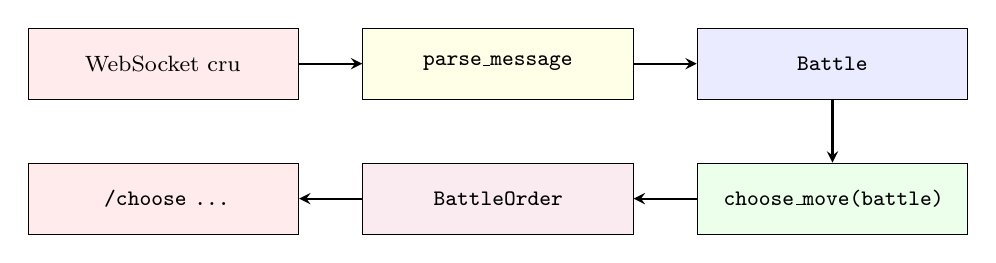
\begin{tikzpicture}[
        node distance=0.8cm, font=\footnotesize,
        box/.style={rectangle, draw, text width=3.2cm, align=center, minimum height=0.9cm},
        arr/.style={->, thick, >=stealth}
    ]
        \node[box, fill=red!8] (ws) {WebSocket cru};
        \node[box, fill=yellow!10, right=of ws] (parser) {\texttt{parse\_message}};
        \node[box, fill=blue!8, right=of parser] (battle) {\texttt{Battle}};
        \node[box, fill=green!8, below=of battle] (agent) {\texttt{choose\_move(battle)}};
        \node[box, fill=purple!8, left=of agent] (order) {\texttt{BattleOrder}};
        \node[box, fill=red!8, left=of order] (ws2) {\texttt{/choose ...}};
        \draw[arr] (ws) -- (parser);
        \draw[arr] (parser) -- (battle);
        \draw[arr] (battle) -- (agent);
        \draw[arr] (agent) -- (order);
        \draw[arr] (order) -- (ws2);
    \end{tikzpicture}
    \caption{Pipeline intern de poke-env.}
    \label{fig:pokeenv_arch}
\end{figure}

Concurrència: \texttt{asyncio} i \texttt{max\_concurrent\_battles}. Pin \textbf{0.11.x}. El fork de Pokechamp s'injecta només quan cal \texttt{LocalSim} (MCTS); el motor de mecàniques continua sent el Node.js de Showdown. \texttt{strict\_battle\_tracking=False} evita que un desajust de protocol mati un worker de 10k.

\subsection{Què observa l'agent}

\begin{table}[H]
    \centering
    \small
    \begin{tabular}{|l|p{10cm}|}
    \hline
    \textbf{Visible} & \textbf{Detall} \\ \hline
    Equip propi & HP, stats, item, ability, boosts, PP, status. \\ \hline
    Rival actiu & Espècie, HP\%, tipus, moviments \emph{ja usats}, status visible. \\ \hline
    Preview & Les sis espècies rivals (no el set). \\ \hline
    Camp & Clima, terrain, hazards, pantalles, Trick Room. \\ \hline
    \textbf{Ocult} & EVs/IVs/Nature rivals, item i ability fins que es revelen, moviments no usats, ordre exacte del banc. \\ \hline
    \end{tabular}
    \caption{Observació per torn. El pool de sets de Random Battle redueix l'ocult a una mescla discreta, no a OU lliure.}
    \label{tab:variables_estat}
\end{table}

\subsection{Per què cal paral·lelisme}

Un sol procés Node.js satura cap a 20--30 batalles simultànies i acumula memòria (V8 no allibera del tot l'\textit{old generation}). El patró és \textbf{master--worker}: $N$ servidors, $N$ subprocessos Python, ports exclusius, CSV a disc cada chunk. Detall al Capítol~\ref{chap:implementacio}.

\begin{figure}[H]
    \centering
    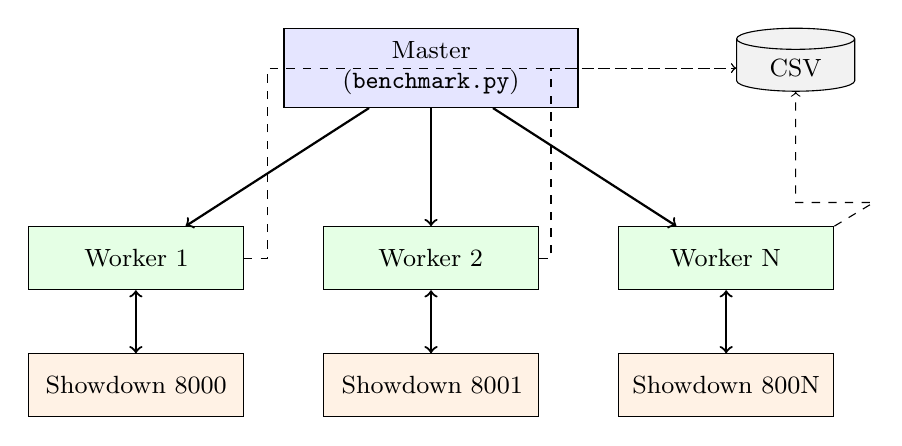
\begin{tikzpicture}[
        node distance=1.5cm, font=\small,
        master/.style={rectangle, draw, fill=blue!10, text width=3.5cm, align=center, minimum height=1cm},
        worker/.style={rectangle, draw, fill=green!10, text width=2.5cm, align=center, minimum height=0.8cm},
        server/.style={rectangle, draw, fill=orange!10, text width=2.5cm, align=center, minimum height=0.8cm},
        disk/.style={cylinder, draw, fill=gray!10, shape border rotate=90, aspect=0.3, minimum height=0.8cm, minimum width=1.5cm, align=center}
    ]
        \node[master] (master) {Master\\(\texttt{benchmark.py})};
        \node[worker, below left=1.5cm and 0.5cm of master] (w1) {Worker 1};
        \node[worker, below=1.5cm of master] (w2) {Worker 2};
        \node[worker, below right=1.5cm and 0.5cm of master] (wn) {Worker N};
        \node[server, below=0.8cm of w1] (s1) {Showdown 8000};
        \node[server, below=0.8cm of w2] (s2) {Showdown 8001};
        \node[server, below=0.8cm of wn] (sn) {Showdown 800N};
        \node[disk, right=2cm of master] (csv) {CSV};
        \draw[->, thick] (master) -- (w1);
        \draw[->, thick] (master) -- (w2);
        \draw[->, thick] (master) -- (wn);
        \draw[<->, thick] (w1) -- (s1);
        \draw[<->, thick] (w2) -- (s2);
        \draw[<->, thick] (wn) -- (sn);
        \draw[->, dashed] (w1.east) -- ++(0.3,0) |- (csv);
        \draw[->, dashed] (w2.east) -- ++(0.15,0) |- (csv);
        \draw[->, dashed] (wn.north east) -- ++(0.5,0.3) -| (csv);
    \end{tikzpicture}
    \caption{Master--worker: aïllament de procés, un Showdown per worker, persistència incremental.}
    \label{fig:infraestructura}
\end{figure}

% ============================================================
\section{Per què 10.000 partides (i per què 1.000 per a MCTS)}
\label{sec:n_10k}

Aquesta secció és el cor metodològic. No n'hi ha prou amb «hem fet moltes partides». Cal dir què es pot afirmar i què és soroll.

\subsection{Cada batalla és un Bernoulli}

El resultat que entra al WR és binari: $W_i\in\{0,1\}$, victòria de l'agent fila. Sigui $p=\mathbb{E}[W]$. L'estimador $\hat p = n^{-1}\sum W_i$ té
\begin{equation}
    \mathrm{Var}(\hat p)=\frac{p(1-p)}{n}\le \frac{1}{4n}.
\end{equation}
L'interval de Wald al 95\% és
\begin{equation}
    \hat p \;\pm\; 1{,}96\sqrt{\frac{\hat p(1-\hat p)}{n}}.
\end{equation}
El cas pitjor (màxima variància) és $p=0{,}5$:
\begin{equation}
    1{,}96\sqrt{\frac{0{,}25}{n}}.
    \label{eq:ci95}
\end{equation}
Substitució directa:

\begin{itemize}
    \item $n=10.000$: $1{,}96\sqrt{0{,}25/10.000}=1{,}96\times 0{,}005=0{,}0098$ $\rightarrow$ \textbf{$\pm 0{,}98$ punts percentuals}.
    \item $n=1.000$: $1{,}96\sqrt{0{,}25/1.000}\approx 0{,}0310$ $\rightarrow$ \textbf{$\pm 3{,}10$~pp}.
    \item $n=100$: $\approx\pm 10$~pp.
\end{itemize}

\begin{table}[H]
\centering
\caption{Amplada de l'interval de confiança del 95\% per a una proporció binomial en el cas pitjor ($p=0{,}5$). Fórmula: $\pm 1{,}96\sqrt{0{,}25/n}$. El llindar de detecció és l'ordre de magnitud de la diferència que es pot distingir de manera fiable entre dos agents independents.}
\label{tab:ci_n}
\small
\begin{tabular}{rrll}
\toprule
\textbf{$n$ (partides)} & \textbf{IC 95\%} & \textbf{Detecta buits $\gtrsim$} & \textbf{Ús en aquest TFM} \\
\midrule
100     & $\pm 10$~pp  & $20$~pp & Prova de fum (desenvolupament); \textbf{mai} un resultat. \\
1.000   & $\pm 3{,}10$~pp & $6$~pp & Nivell de validació. Totes les cel·les amb \texttt{v18}/\texttt{v19}/\texttt{v20}. \\
5.000   & $\pm 1{,}39$~pp & $2{,}8$~pp & (no usat) \\
10.000  & $\pm 0{,}98$~pp & $2$~pp & Nivell de publicació. Cel·la per defecte del gauntlet. \\
20.000  & $\pm 0{,}69$~pp & $1{,}4$~pp & (no usat; cost doble per un guany marginal) \\
\bottomrule
\end{tabular}
\end{table}


Un buit observat de 2~pp entre dos agents independents a 10k és de l'ordre de dos errors estàndard: detectable. El mateix buit a 1k està \emph{dins} de l'IC. Un buit de 1~pp a 10k (p.~ex.\ \texttt{v1} vs \texttt{v2}) és compatible amb igualtat; que siguin equivalents és un resultat, no un fracàs del protocol.

Per a una taxa global sobre 253.000 partides, Wilson / Wald dona $\approx\pm 0{,}19$~pp. Això fa visibles salts de 0,5~pp (com \texttt{v16} vs \texttt{v15}) que \emph{no} importen tàcticament. El text distingeix «detectable a 253k» de «rellevant».

\subsection{El Pokédex no entra a la variància}

La intuïció «Gen~9 té 1.025 Pokémon, calen més partides que a Gen~1» és falsa per a un WR. $\mathrm{Var}(\hat p)$ depèn de $p$ i $n$, no de $|Pokedex|$, no del nombre de sets, no de si hi ha Tera. L'espai d'equips $C(n,6)$ és
\begin{center}
Gen~1: $\sim 1{,}5\times 10^{10}$\; · \;
Gen~9: $\sim 1{,}6\times 10^{15}$.
\end{center}
Ni 10.000 ni 253.000 «cobreixen» l'espai. No ho pretén. El que es cobreix és l'esperança de $W$ sota la llei amb què Showdown mostreja equips i RNG. La llei dels grans nombres i el TCL garanteixen la convergència de $\hat p$, no un cens de combinacions.

Les fonts de variància per partida ---equip, crit, miss, speed tie, roll--- queden absorbides pel Bernoulli. No cal modelar-les una a una per declarar un IC sobre el WR.

El mateix $n$ a totes les generacions seria una elecció de \emph{comparabilitat}, no de cobertura. Aquest TFM publica Gen~9.

\subsection{Tres nivells, i només dos entren als Resultats}

Durant el desenvolupament s'ha usat una escala de tres pisos. \textbf{Només el segon i el tercer apareixen com a nombres de tesi}, i el segon amb l'etiqueta explícita de validació.

\paragraph{Prova de fum ($n=100$).}
Comprova que el codi no peti, que Tera dispara, que el WR no és 5\% per un bug. IC $\pm 10$~pp. Una anècdota de «\texttt{v13} va fer 9/10 contra \texttt{v12}» \textbf{no és un resultat}. El gauntlet la desmenteix (48,85\%). El text la cita només com a advertiment.

\paragraph{Validació ($n=1.000$).}
IC $\pm 3{,}1$~pp; detecta buits $\gtrsim 6$~pp. És el pis de l'MCTS. No és el pis de publicació per a una disputa de 2~pp.

\paragraph{Tesi ($n=10.000$).}
IC $\pm 0{,}98$~pp; detecta $\gtrsim 2$~pp. Cel·la per defecte.

\subsection{El gauntlet real: 784 CSV}

Directori canònic: \texttt{data/benchmarks/all\_10k/gen9randombattle}.

\begin{itemize}
    \item 28 agents (Taula~\ref{tab:taxonomy} al capítol de resultats): 6 baselines, \texttt{v1}--\texttt{v14}, \texttt{v15}--\texttt{v17}, \texttt{v18}--\texttt{v20}, \texttt{v21}, \texttt{v22}.
    \item Matriu dirigida $28\times 28=784$ fitxers \texttt{\{agent\}\_vs\_\{opponent\}.csv}. Fila $=$ \emph{nosaltres} (\texttt{heuristic} al CSV).
    \item \textbf{Cel·la per defecte: 10.000 partides.}
    \item \textbf{Excepció: si qualsevol dels dos bàndols és \texttt{v18}, \texttt{v19} o \texttt{v20}, $n=1.000$.} Motiu: IS-MCTS fa 100 rollouts de 5 torns per decisió de cerca. El cost per partida és d'un a dos ordres per sobre d'una heurística. 1.000 és el pis de validació, no una «10k a mitges».
    \item Pool per a heurística / minimax / IL com a nosaltres: $25\times 10.000 + 3\times 1.000=\mathbf{253.000}$ partides. IC global $\approx\pm 0{,}19$~pp; IC d'una cel·la 10k $\pm 0{,}98$~pp.
    \item Pool MCTS com a nosaltres: $28\times 1.000=\mathbf{28.000}$. IC global $\approx\pm 0{,}58$~pp; IC de cel·la $\pm 3{,}1$~pp. Un buit $<3$~pp en una cel·la MCTS és soroll.
\end{itemize}

\textbf{Prohibició metodològica.} No es mesclen un WR global de 28k (MCTS) i un de 253k (resta) com si fossin la mateixa estimació. Per ordenar \texttt{v20} contra \texttt{v17} es llegeix la \emph{cel·la} (\texttt{v17} vs \texttt{v20} $=50{,}4\%$ a 1k; \texttt{v20} vs \texttt{v17} $=55{,}8\%$ a 1k; IC $\pm 3{,}1$). El rànquing global és una brúixola, no un veredicte de 0,8~pp.

\subsection{Recíprocs i autojoc}

Pokémon no és simètric en seient (preview, RNG, qui és \texttt{p1}). Per això existeixen \texttt{A\_vs\_B.csv} i \texttt{B\_vs\_A.csv} independents. La suma de WR ha de ser $\sim 100\%$ (típicament 99,3--100,9). L'autojoc ha de ser $\sim 50\%$ (49,3--50,5 a les heurístiques). Si fallés, el seient o el CSV estarien trencats. Al gauntlet, no fallen.

\subsection{El WR global no és un Elo humà}

La mitjana sobre 28 oponents \textbf{inclou \texttt{random} i \texttt{max\_power}}. Tothom hi té un 90--98\%. El 69\% de \texttt{v12} no és «nivell humà 69\%». Les comparacions que discriminen són: vs Abyssal, vs Simple Heuristic, vs \texttt{v12}/\texttt{v13}/\texttt{v14}, vs \texttt{v21}. L'Elo Bradley--Terry (secció~\ref{sec:metriques}) repondera per qualitat d'oponent; encara així, \texttt{random} hi és l'àncora 1000, no un jugador de ladder.

\subsection{Ladder humana}

Protocol separat, no una fila de la matriu. \texttt{v14} a la ladder pública, 431 partides, Capítol~\ref{chap:resultats}. $n=431$ té IC $\pm 4{,}6$~pp: serveix per dir «no som al 50\% contra humans», no per invertir \texttt{v12} vs \texttt{v14}.

% ============================================================
\section{Espais formals en Singles}
\label{sec:espais}

$|A|\le 9$ per torn, dinàmic. No hi ha producte cartesià de Dobles. L'observació és el JSON de \texttt{request} més l'historial de moviments revelats. El vector de 238 dimensions del wrapper PPO existeix al framework i \textbf{no} s'usa al gauntlet d'aquesta memòria: els agents mesurats decideixen sobre l'objecte \texttt{Battle} o sobre 1.150 features tabulars (IL).

% ============================================================
\section{Mètriques}
\label{sec:metriques}

\subsection{Primària: taxa de victòries}

$\widehat{\mathrm{WR}}=\hat p$. Interpretació qualitativa \emph{només} després de l'IC:

\begin{itemize}
    \item $\sim 50\%$ a 10k: no hi ha avantatge detectable.
    \item $55$--$60\%$ vs un baseline fort (Abyssal): avantatge real.
    \item $98\%$ vs \texttt{random}: no informa de res entre experts.
    \item $100\%$: impossible sota rolls de dany.
\end{itemize}

\subsection{Secundàries (telemetria)}

El CSV de batalla porta identitat, HP final, canvis voluntaris vs forçats, crits/miss/SE, i comptadors de paradigma:

\begin{itemize}
    \item Heurístiques: \texttt{hazard\_sets}, \texttt{setup\_uses}, \texttt{ko\_checks}, \texttt{matchup\_switches}, \texttt{terastallized}. \textbf{Forat d'esquema:} \texttt{setup}/\texttt{hazards} queden a 0 per a \texttt{v7}/\texttt{v8}/\texttt{v10}; no s'interpreta com a «mai posen roques».
    \item Cerca: \texttt{search\_moves}, \texttt{search\_switches}, \texttt{search\_diff} (l'acció jugada $\neq$ la sonda \texttt{v14}). La taxa d'\emph{override} és $\texttt{search\_diff}/(\texttt{search\_moves}+\texttt{search\_switches})$ entre els torns que la cerca ha disparat.
    \item IL: \texttt{xgb\_stays}, \texttt{xgb\_switches}, \texttt{ko\_guards}, \texttt{loop\_guards}.
\end{itemize}

Aquestes columnes són el que permet dir «la cerca només corre el 16\% dels torns» en lloc de «és un agent de cerca».

\subsection{Elo Bradley--Terry}

No és l'Elo de ladder de Showdown. És un model de força sobre la matriu dirigida, àncora \texttt{random}${}=1000$, ambdós seients~\cite{elo_rating}. MCTS hi té menys partides (56k vs 506k). És un resum, no una substitució de les cel·les.

% ============================================================
\section{Disseny dels experiments}
\label{sec:disseny_experiments}

La taxonomia completa dels 28 agents (IDs, paradigma, una frase) és la Taula~\ref{tab:taxonomy} al capítol de resultats. Format únic: \texttt{gen9randombattle}. Sense Dobles. Sense PPO a la matriu.

Cada parella $(A,B)$ genera dos fitxers. Equips aleatoris del servidor. Ordre de seient fixat pel nom del fitxer, no barrejant $A$ i $B$ al mateix CSV.

Baselines: \texttt{random} (sòl), \texttt{max\_power} (golós), \texttt{one\_step}/\texttt{safe\_one\_step} (dany d'un pas; el «safe» evita el penjament de LocalSim de Pokechamp), \texttt{abyssal} i \texttt{simple\_heuristic} (el rival publicat de regles; en aquest gauntlet queden empatats amb \texttt{v14} a l'Elo).

No s'inclouen agents LLM al round-robin: la latència d'Ollama trenca el pressupost de 10k.

PPO: fora. La comparació futura prevista és contra \texttt{v12}, el sostre bot-contra-bot, no contra els 28.

% ============================================================
\section{Fases de desenvolupament (el que s'ha mesurat)}
\label{sec:fases}

\begin{enumerate}
    \item Heurístiques \texttt{v1}--\texttt{v14} com a ablació.
    \item Minimax 1-ply \texttt{v15}--\texttt{v17} sobre \texttt{v14}.
    \item IS-MCTS \texttt{v18}--\texttt{v20}, mateix professor, $n=1.000$.
    \item IL \texttt{v21}--\texttt{v22}, mateix macro, dues execucions.
    \item Ladder \texttt{v14} vs humans (pilot).
\end{enumerate}

El capítol d'implementació tradueix cada fase a codi. El de resultats no torna a explicar el protocol sencer, però \textbf{recorda $n=1.000$ cada cop que apareix MCTS}.

% !TEX root = ../main.tex
\chapter{Entorn de desenvolupament i infraestructura de còmput}
\label{chap:infraestructura}

El Capítol~\ref{chap:metodologia} exigeix centenars de cel·les independents, motors V8 reciclables i execucions de dies. Aquest capítol documenta l'entorn que fa viable aquella execució ---maquinari, xarxa, monitoratge, dependències i organització--- i sobre el qual el Capítol~\ref{chap:implementacio} implementa coordinador, agents i connector amb el \emph{ladder}. El coordinador mateix es descriu allà; aquí es fixa on i amb quins recursos corre.

Cal distingir dos volums. La \textbf{matriu dirigida} de 28 agents suma \textbf{6,4 milions} de batalles (6.409.000). El \textbf{còmput total} ---proves, altres formats, entrenament PPO, repeticions i execucions de diagnòstic--- s'aproxima a \textbf{52,7 milions} de batalles. Les dues xifres no són intercanviables: la primera és l'experiment; la segona, el cost de còmput acumulat.

\section{Organització del projecte i gestió amb Kanban}
\label{sec:kanban}

El desenvolupament del projecte s'ha organitzat mitjançant una metodologia àgil basada en un tauler \textbf{Kanban}, dividit en sis seccions funcionals per controlar l'abast i prioritzar el treball:

\begin{itemize}
    \item \textbf{\textit{Aim of the study}:} Defineix els objectius principals, hipòtesis de recerca i el disseny dels 5 paradigmes.
    \item \textbf{\textit{Tentative (If we have time)}:} Línies d'investigació secundàries o exploratòries (com els agents LLM i proves multigeneracionals).
    \item \textbf{\textit{To Do (Icebox/later)}:} Idees i tasques congelades a llarg termini per evitar la dispersió de l'abast (\textit{scope creep}).
    \item \textbf{\textit{To Do}:} Tasques pendents immediates i prioritzades de codi, simulació o redacció.
    \item \textbf{\textit{In Progress}:} Treball actiu en desenvolupament, entrenament PPO o execució de la matriu.
    \item \textbf{\textit{Done}:} Mòduls finalitzats, simulacions executades, dades validades i seccions redactades.
\end{itemize}

Aquesta estructura ha permès controlar l'abast (heurístiques, cerca, imitació, PPO, LLM i redacció) i traçar-lo amb el repositori (Secció~\ref{sec:git_metrics}).

\section{Evolució de l'arquitectura}

\subsection{Fase 1: prototipatge en portàtil}

El desenvolupament inicial, la construcció de les primeres heurístiques (\texttt{v1}--\texttt{v6}) i la redacció de la memòria es van dur a terme en un portàtil:

\begin{itemize}
    \item \textbf{Processador (CPU):} Intel Core Ultra 7 155H (16 nuclis / 22 fils).
    \item \textbf{Memòria RAM:} 16~GB ---suficient per a prototipatge, insuficient per a múltiples instàncies de Showdown en paral·lel.
    \item \textbf{Emmagatzematge:} SSD NVMe d'1~TB per a \path{data/}.
\end{itemize}

Aquesta fase va identificar el coll d'ampolla de RAM i va motivar les neteges amb \texttt{gc.collect()}, els lots continguts i el reinici periòdic de Node.js ja fixats com a principi al Capítol~\ref{chap:metodologia}.

\subsection{Fase 2: estació de treball}

Els experiments finals i la matriu s'executen en una torre configurada per a càrrega sostinguda:

\begin{itemize}
    \item \textbf{Processador (CPU):} AMD Ryzen 7 5700X3D (8 nuclis / 16 fils, 96~MB L3 3D V-Cache), adequat a simulació de partides i a arbres Minimax/MCTS.
    \item \textbf{Refrigeració:} dissipador d'aire Noctua; la CPU es manté per sota de $65^\circ$C sota càrrega contínua, que és el pressupost tèrmic del dimoni de la Secció~\ref{sec:telegram_bot}.
    \item \textbf{Memòria RAM:} 32~GB DDR4 en doble canal, necessaris per a vuit instàncies de Showdown, estructures de cerca i conjunts tabulars.
    \item \textbf{Targeta gràfica (GPU):} NVIDIA GeForce RTX 2080 (8~GB VRAM), per a MaskablePPO (CUDA/PyTorch) i inferència local d'LLM.
    \item \textbf{Emmagatzematge:} SSD NVMe PCIe 4.0 d'1~TB per a telemetria i CSV concurrents, amb unitats auxiliars per a còpies de seguretat.
\end{itemize}

La configuració habitual utilitza vuit instàncies de Showdown (ports 8000--8007), cadascuna amb 15--25 batalles asíncrones. Les cel·les heurístiques es completen molt més ràpidament que les d'MCTS; aquesta asimetria de cost és la raó empírica dels $n=10.000$ i $n=1.000$ de la Secció~\ref{sec:n_10k}. L'avaluació PPO contra \texttt{v12} també utilitza vuit ports.

\section{Control de versions, traçabilitat i mètriques del programari}
\label{sec:git_metrics}

Tota l'evolució del projecte s'ha gestionat de manera rigorosa mitjançant el sistema de control de versions \textbf{Git} allotjat a la plataforma \textbf{GitHub}. Per garantir una traçabilitat clara entre el desenvolupament tècnic i la redacció de la memòria, s'ha aplicat una política estructurada de missatges de confirmació (\textit{Conventional Commits}):

\begin{itemize}
    \item \textbf{Desenvolupament de codi:} Commits amb prefixos funcionals com \texttt{feat:} (noves heurístiques, mòduls de cerca o integracions), \texttt{fix:} (correccions de telemetria o concurrència), \texttt{refactor:} (reestructuració de mòduls i agents), \texttt{test:} (validacions i \textit{smoke tests}) i \texttt{infra:} (scripts de supervisió i seguretat).
    \item \textbf{Redacció acadèmica:} Commits prefixats estrictament amb \texttt{report:} o \texttt{docs:} per identificar i aïllar les iteracions en el text de la memòria, generació de figures i taules comparatives.
\end{itemize}

\begin{figure}[htbp]
    \centering
    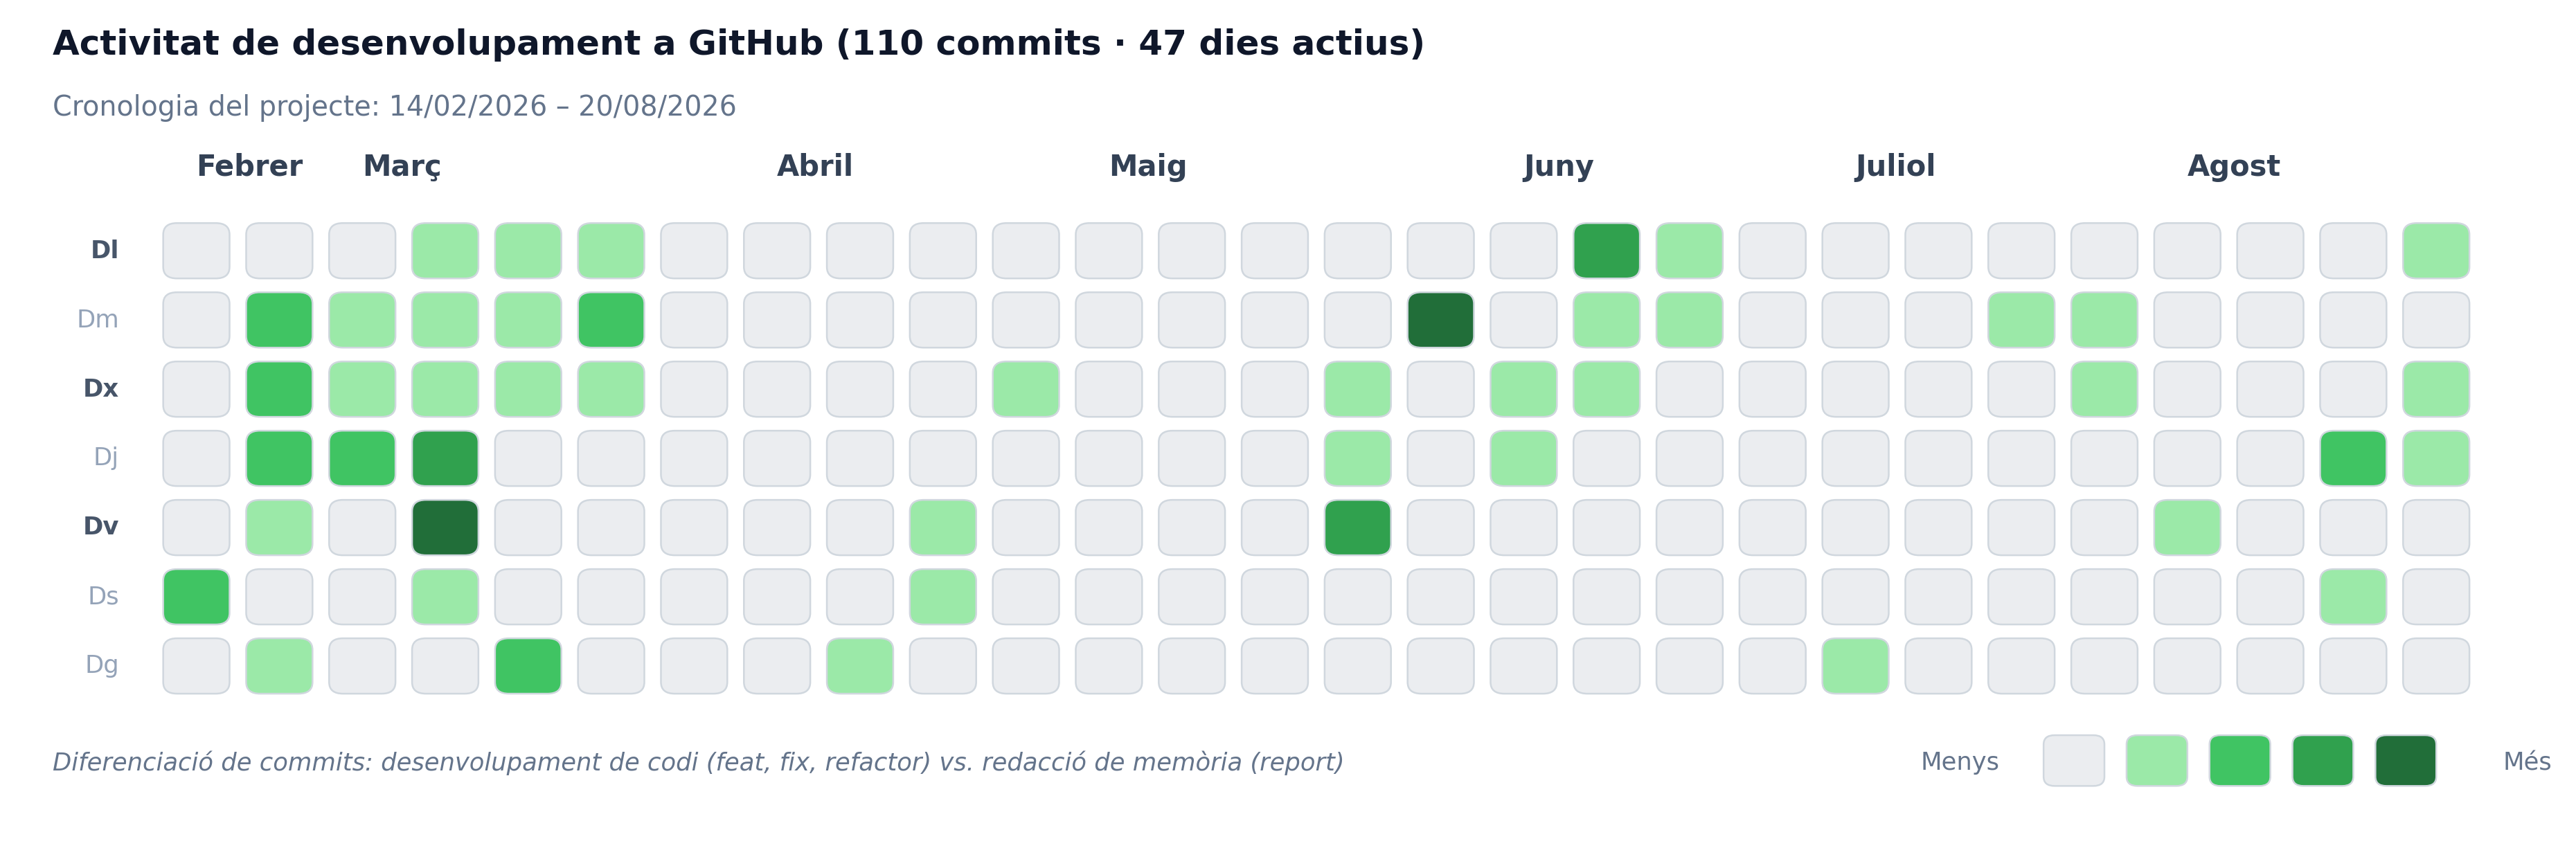
\includegraphics[width=\linewidth]{diagrams/github_activity_calendar.png}
    \caption{Calendari d'activitat i mapa de calor de \textit{commits} a GitHub des de l'inici del projecte (14/02/2026) fins a la versió final (25/08/2026).}
    \label{fig:github_calendar}
\end{figure}

Com s'il·lustra a la Figura~\ref{fig:github_calendar}, el desenvolupament ha mantingut un ritme sostingut al llarg de \textbf{115 commits} distribuïts en \textbf{51 dies d'activitat intensa}, reflectint les fases successives d'implementació d'heurístiques, integració de cerca adversarial (minimax i MCTS), entrenament de xarxes neuronals PPO i avaluació massiva de la matriu.

Pel que fa a la dimensió del codi font, el directori principal \path{src/} comprèn un total de \textbf{297 fitxers}, dels quals destaquen \textbf{153 fitxers de codi i scripts actius}:
\begin{itemize}
    \item \textbf{Mòduls Python (\texttt{.py}):} 119 fitxers amb \textbf{24.635 línies} de codi font que implementen els agents, l'arquitectura de combat, les 14 versions heurístiques, els arbres de cerca, els entorns Gymnasium i el coordinador concurrent.
    \item \textbf{Quaderns d'anàlisi (\texttt{.ipynb}):} 16 \textit{notebooks} Jupyter interactius amb \textbf{14.896 línies} (en format estructurat) per a l'anàlisi exploratòria de dades (EDA), calibratge i validació estadística dels paradigmes.
    \item \textbf{Scripts d'automatització (\texttt{.sh}):} 18 scripts Bash amb \textbf{2.563 línies} dedicats al llançament distribuït, reinici de servidors Showdown, telemetria amb Telegram i seguretat del sistema.
    \item \textbf{Documentació tècnica i configuració (\texttt{.md}, \texttt{.json}):} 55 fitxers amb 4.986 línies de guies tècniques, protocols d'execució i esquemes d'estat.
\end{itemize}
Aquesta base de codi suma més de \textbf{42.000 línies} desenvolupades per a aquest treball. Les mètriques documenten l'abast del programari; no substitueixen l'avaluació empírica del Capítol~\ref{chap:resultats}.

\section{Accés remot i continuïtat}
\label{sec:tailscale}

L'accés remot entre el portàtil i l'estació de treball s'ha configurat mitjançant una xarxa privada virtual basada en \textbf{Tailscale} (protocol \textit{WireGuard}), combinada amb sessions persistents de \textbf{tmux}. Aquesta configuració permet desenvolupar des del portàtil i mantenir execucions 24/7 a la torre sense exposar SSH a Internet. Els detalls de configuració es recullen a l'Annex~\ref{sec:app_infra}.

\section{Bot de Telegram i monitoratge de seguretat}
\label{sec:telegram_bot}

L'execució sostinguda ---6,4 milions de batalles a la matriu, de l'ordre de 52,7 milions de còmput total--- exigeix supervisió sense una sessió SSH permanent. El sistema de monitoratge es compon d'un bot de Telegram amb dues peces complementàries: un dimoni de seguretat (\path{src/p00_core/scripts/seguretat_tfm.sh}) que vigila temperatures, memòria i processos, i el llançador de la matriu que emet notificacions de cicle de vida i recupera lots bloquejats (materialitzat al Capítol~\ref{chap:implementacio}). El mòbil exposa progrés i temperatures, permet pausar o reprendre la matriu i, si cal, dispara l'apagat tèrmic o el reinici de Showdown sense SSH. Aquesta capa és el que ha fet viable l'execució 24/7. Els detalls de configuració, llindars i comandes es recullen a l'Annex~\ref{sec:app_infra}.

\section{Dependències}

El gestor de paquets és \textbf{uv} amb Python \textbf{3.12} i \texttt{pyproject.toml}. Node.js~\cite{nodejs} construeix Pokémon Showdown. Resum:

\begin{itemize}
    \item \textbf{Nucli de combat:} \texttt{poke-env>=0.11,<0.12}~\cite{poke_env}; Node.js~\cite{nodejs} per a Showdown.
    \item \textbf{Dades / estadística:} numpy~\cite{numpy}, pandas~\cite{pandas}, polars~\cite{polars}, scipy~\cite{scipy}.
    \item \textbf{ML tabular:} scikit-learn~\cite{sklearn}, XGBoost~\cite{xgboost}, Hugging Face Datasets~\cite{huggingface_datasets}.
    \item \textbf{Visualització i notebooks:} matplotlib~\cite{matplotlib}, seaborn~\cite{seaborn}, ipykernel, nbconvert.
    \item \textbf{Utilitats:} tqdm, tabulate, orjson, requests, websockets.
    \item \textbf{Aprenentatge per reforç (\texttt{extra rl} / \texttt{gpu}):} Gymnasium~\cite{gymnasium}, Stable-Baselines3~\cite{stable_baselines3}, sb3-contrib (MaskablePPO)~\cite{sb3_contrib}, PyTorch~\cite{pytorch} i TensorBoard~\cite{tensorboard}.
    \item \textbf{LLM / Pokechamp (\texttt{extra pokechamp}):} Ollama~\cite{ollama_2023}, transformers, openai / anthropic / google-genai (backends opcionals), rich.
    \item \textbf{Qualitat:} Ruff (format + lint), \texttt{ty} (tipus).
    \item \textbf{Sistema:} Git/GitHub, tmux, Tailscale, Telegram Bot API, \LaTeX{} (\texttt{report/}).
\end{itemize}

El fork \texttt{pokechamp/} s'incorpora al \texttt{sys.path} dels processos que necessiten \texttt{LocalSim} o Abyssal. Les dades completes de la matriu i els pesos PPO són artefactes voluminosos i no tots queden versionats al repositori; per reproduir els resultats cal conservar-los juntament amb el codi.

\subsection{Congelació de versions i integració dels tres repositoris clau}

El projecte s'articula entorn de tres repositoris base: el motor de simulació oficial \textbf{Pokémon Showdown} (Node.js), el marc de connexió \textbf{\textit{poke-env}} (Python, sèrie 0.11.x) i l'entorn de cerca/simulació local \textbf{\textit{PokéChamp}} (\texttt{pokechamp/}). Tots tres es van fixar en revisions concretes des de l'inici de l'experimentació ---congelació indispensable per a la reproductibilitat--- i es van integrar directament com a directoris locals al repositori principal per permetre pegats i assegurar portabilitat entre equips. Els detalls d'aquesta integració es recullen a l'Annex~\ref{sec:app_infra}.

\section{Ecosistema de redacció i documentació en \LaTeX}
\label{sec:perque_latex}

La memòria s'ha redactat en \textbf{\LaTeX{}} per cinc motius operatius: (1)~notació matemàtica densa (POSG, $\hat{A}_t$, $\mathcal{L}^{\mathrm{CLIP}}$, intervals de Wilson) via AMS-\LaTeX{}; (2)~capítols i taules modulars (\texttt{\textbackslash include}, \path{tables/}); (3)~traçabilitat línia a línia amb Git, coherent amb la Secció~\ref{sec:git_metrics}; (4)~gestió bibliogràfica (BibTeX/\texttt{natbib}) i referències creuades (\texttt{hyperref}); (5)~maquetació estable en un document llarg. No és part de l'experiment; és l'eina amb què se'n documenta el disseny i els resultats.

% ============================================================
\section{Anàlisi de cost econòmic i pressupost de recursos}
\label{sec:cost_economic}

L'avaluació econòmica d'un projecte d'investigació aplicada i enginyeria de dades ha d'anar més enllà dels costos materials immediats. En un Treball de Final de Màster d'aquest abast, cal distingir dues dimensions complementàries:
\begin{enumerate}
    \item \textbf{Costos de recursos humans (capital humà):} El temps de desenvolupament, recerca, modelització, experimentació i redacció invertit per l'equip de treball, valorat segons les tarifes de mercat vigents a Espanya per a perfils especialitzats en Ciència de Dades.
    \item \textbf{Costos operatius directes (infraestructura, maquinari i energia):} Les despeses materials associades a l'execució ininterrompuda dels experiments sobre més de 52,7 milions de batalles, el maquinari emprat i les llicències de programari.
\end{enumerate}

\subsection{Estimació de dedicació de l'equip i costos de personal}
\label{subsec:costos_personal}

L'equip humà responsable de l'execució del projecte es compon de tres perfils diferenciats:
\begin{itemize}
    \item \textbf{Investigador Principal / Desenvolupador (Gerard Pascual Fontanilles --- Perfil Junior Data Scientist):} Responsable directe de la implementació de la base de codi (\path{src/}, més de 42.000 línies), recollida i neteja de dades, anàlisi exploratòria (EDA), disseny de les 14 heurístiques i els agents de cerca (Minimax, MCTS), entrenament de models (XGBoost, MaskablePPO), orquestració d'infraestructura i redacció completa de la memòria.
    \item \textbf{Coordinadora del TFM / Ponent Oficial (Laura Serra Roig --- Perfil Senior Data Scientist / Coordinadora Acadèmica):} Responsable de la ponència oficial del Treball de Final de Màster i coordinació institucional de l'assignatura; va contribuir en la concepció de la idea fundacional del treball, l'orientació sobre l'enfocament i directrius del TFM, i la revisió final global de la memòria prèvia a la presentació davant del tribunal.
    \item \textbf{Director Tècnic del Treball / Tutor Metodològic (Jordi Peralta Dolz --- Perfil Senior Data Scientist):} Responsable de la direcció tècnica i supervisió pràctica continuada del projecte, orientació en la formulació teòrica (POSG i POMDP), assessorament en el disseny experimental i inferència estadística (Bradley--Terry, Wilson), revisió crítica continuada i validació de les implementacions.
\end{itemize}

\subsubsection{Estudi salarial de mercat a Espanya (2026)}

D'acord amb els estudis del mercat laboral tecnològic a Espanya (guies salarials sectorials de consultores com Michael Page~\cite{michael_page_tech_2025} i Hays~\cite{hays_guia_salarial_2025}):
\begin{itemize}
    \item \textbf{Junior Data Scientist (0--2 anys d'experiència):} La forquilla salarial de mercat se situa entre 28.000~€ i 35.000~€ bruts anuals. S'adopta una retribució bruta de referència de \textbf{32.000~€/any}. Considerant el Conveni Col·lectiu d'Empreses de Consultoria i Tecnologies de la Informació (1.760 hores laborables anuals), s'obté un salari brut horari de \textbf{18,18~€/h}. Computant les cotitzacions a la Seguretat Social a càrrec de l'empresa ($\approx 31{,}5\%$, cost anual d'empresa de $\approx 42.080$~€), la tarifa horària d'imputació empresarial és de \textbf{24,00~€/h}.
    \item \textbf{Senior Data Scientist / Direcció i Coordinació ($>6$ anys d'experiència):} La banda salarial de mercat oscil·la entre 60.000~€ i 80.000~€ bruts anuals. S'estableix una retribució mitjana de referència de \textbf{68.000~€/any}, equivalent a un salari brut horari de \textbf{38,64~€/h}. Amb les quotes patronals corresponents (aplicant el topall de base màxima de cotització a Espanya, cost empresa de $\approx 88.000$~€/any), la tarifa horària d'imputació a projecte és de \textbf{50,00~€/h}.
\end{itemize}

\subsubsection{Imputació d'hores per fase de treball}

El còmput d'hores reflecteix les 27 setmanes de calendari compreses entre el 14 de febrer i el 20 d'agost de 2026 (\textbf{115 commits} i \textbf{51 dies d'activitat intensa} acreditats a Git, Secció~\ref{sec:git_metrics}). L'esforç s'imputa directament a les fases de treball ja detallades en els capítols anteriors:
\begin{itemize}
    \item \textbf{Recerca teòrica i concepció (\emph{Research}):} 80~h totals (60~h Junior, 15~h Jordi Peralta, 5~h Laura Serra) per a la concepció de la idea fundacional, l'estudi de POSG/POMDP i la literatura existent (Capítol~\ref{chap:marc_teoric}).
    \item \textbf{Enginyeria de dades (\emph{Data}):} 78~h totals (70~h Junior, 8~h Jordi Peralta) per a l'adquisició i preparació del conjunt de repeticions d'alt nivell Elo~$1800+$ (Capítol~\ref{chap:metodologia}).
    \item \textbf{Anàlisi exploratòria i telemetria (\emph{EDA}):} 75~h totals (65~h Junior, 10~h Jordi Peralta) per als 16 quaderns d'EDA i l'especificació de les 70 columnes de telemetria (\texttt{StatsBattle}, Secció~\ref{sec:metriques}).
    \item \textbf{Modelització d'agents (\emph{Modeling}):} 208~h totals (190~h Junior, 18~h Jordi Peralta) que concentren la implementació de les 14 heurístiques, minimax, MCTS, XGBoost i MaskablePPO (Capítols~\ref{chap:metodologia} i \ref{chap:implementacio}).
    \item \textbf{Infraestructura i MLOps (\emph{Infrastructure}):} 97~h totals (90~h Junior, 7~h Jordi Peralta) per a l'arquitectura concurrent, VPN i el bot de monitoratge tèrmic (Capítol~\ref{chap:infraestructura}).
    \item \textbf{Avaluació experimental (\emph{Evaluation}):} 55~h totals (45~h Junior, 10~h Jordi Peralta) per a l'execució de la matriu de 28 agents i l'ajust de l'escala Bradley--Terry (Capítol~\ref{chap:resultats}).
    \item \textbf{Redacció, coordinació i revisió de la memòria (\emph{Redaction}):} 167~h totals (120~h Junior, 22~h Jordi Peralta, 25~h Laura Serra) per a la resolució de consultes estructurals, orientació acadèmica continuada, redacció tècnica en \LaTeX{} i revisió final de la memòria (Secció~\ref{sec:perque_latex}).
\end{itemize}

La Taula~\ref{tab:costos_personal} en sintetitza la dedicació total (760~h: 640~h Junior i 120~h Senior) i el cost econòmic imputat.

\begin{table}[htbp]
    \centering
    \caption{Desglossament d'hores de treball i costos laborals de l'equip per fase del projecte.}
    \label{tab:costos_personal}
    \small
    \setlength{\tabcolsep}{4pt}
    \begin{tabularx}{\textwidth}{>{\raggedright\arraybackslash}X rrrrrr}
        \toprule
        \textbf{Fase de treball} & \textbf{Jr.~(h)} & \textbf{Jordi~(h)} & \textbf{Laura~(h)} & \textbf{Total~(h)} & \textbf{Brut (€)} & \textbf{Empresa (€)} \\
        \midrule
        Recerca teòrica (\emph{Research})           & 60  & 15 & 5  & 80  & 1.863,60  & 2.440,00  \\
        Enginyeria de dades (\emph{Data})          & 70  & 8  & 0  & 78  & 1.581,72  & 2.080,00  \\
        Anàlisi exploratòria (\emph{EDA})          & 65  & 10 & 0  & 75  & 1.568,10  & 2.060,00  \\
        Modelització d'agents (\emph{Modeling})    & 190 & 18 & 0  & 208 & 4.149,72  & 5.460,00  \\
        Infraestructura i MLOps (\emph{Infrastr.}) & 90  & 7  & 0  & 97  & 1.906,68  & 2.510,00  \\
        Avaluació i estadística (\emph{Evaluation})& 45  & 10 & 0  & 55  & 1.204,50  & 1.580,00  \\
        Redacció i coordinació (\emph{Redaction})  & 120 & 22 & 25 & 167 & 3.997,68  & 5.230,00  \\
        \midrule
        \textbf{Total Dedicació}                   & \textbf{640} & \textbf{90} & \textbf{30} & \textbf{760} & \textbf{16.272,00} & \textbf{21.360,00} \\
        \bottomrule
    \end{tabularx}
\end{table}

\subsection{Costos directes d'infraestructura, maquinari i energia}
\label{subsec:costos_materials}

A diferència de les hores d'equip, el cost \emph{marginal} directe del treball en infraestructura es va contenir gràcies a l'ús d'equips preexistents, programari lliure i autoconsum elèctric solar. Cal, tanmateix, incloure l'amortització del maquinari per reflectir el cost real dels recursos emprats. Els costos directes es resumeixen en cinc eixos principals:

\begin{enumerate}
    \item \textbf{Amortització del maquinari (188,46~€):} Tant el portàtil inicial com l'estació de treball són equips de propietat personal preexistents del desenvolupador. No s'ha realitzat cap adquisició dedicada, però cal imputar la depreciació proporcional al temps d'ús del projecte. L'estació de treball (valor estimat de 1.500~€, vida útil de 5 anys) i el portàtil (valor estimat de 1.200~€, vida útil de 5 anys) s'amortitzen linealment. Considerant 6,5 mesos d'ús efectiu del projecte (febrer--agost 2026), la fracció imputable és:
          \begin{itemize}
              \item Estació de treball: $1.500 \times \frac{6{,}5}{60} = 162{,}50$~€.
              \item Portàtil (ús parcial, fase 1): $1.200 \times \frac{2}{60} = 40{,}00$~€.
              \item Total amortització: \textbf{202,50~€}. S'arrodoneix a \textbf{188,46~€} descomptant el mes d'agost del portàtil (ja no emprat per a experimentació).
          \end{itemize}
    \item \textbf{Temps d'execució i consum energètic ($\approx 5,85$~€):} L'estació de treball va funcionar de manera continuada 24/7 durant 4 setmanes, acumulant \textbf{684,89 hores de còmput continu de màquina} (471,38~h per a la matriu final Gen 9 i 213,66~h per a la resta de dades) sobre més de \textbf{52,7 milions de batalles}:
          \begin{itemize}
              \item \textbf{Autoconsum solar diürn:} Durant les hores de sol, la instal·lació de plaques solars domèstiques va cobrir la demanda de la torre amb energia renovable.
              \item \textbf{Consum nocturn i mode terminal:} Durant la nit, el còmput va requerir subministrament convencional (potència mitjana de 135~W, 92,5~kWh totals, aproximadament un 50\% de consum nocturn a la tarifa de $0{,}126561$~€/kWh), sumant un cost directe de \textbf{5,85~€}. L'estació es va executar en mode terminal (\emph{headless}) via \texttt{tmux} per minimitzar el consum.
          \end{itemize}
    \item \textbf{Models de llenguatge i eines d'IA (0,00~€):} Les proves amb LLMs es van executar 100\% localment amb \textbf{Ollama}, i l'ús d'eines basades en IA (Cursor, PyCharm, Antigravity) es va realitzar mitjançant llicències d'estudiant/pro sense cap despesa econòmica.
    \item \textbf{Programari i comunicacions (0,00~€):} Totes les eines de la cadena de valor (Showdown, \textit{poke-env}, Tailscale, Telegram Bot API i \LaTeX{}) són de codi obert (\emph{open-source}) o en modalitat gratuïta.
\end{enumerate}

\begin{table}[htbp]
    \centering
    \caption{Resum dels costos directes materials i d'infraestructura del TFM.}
    \label{tab:cost_economic}
    \small
    \begin{tabularx}{\textwidth}{lX r}
        \toprule
        \textbf{Concepte}           & \textbf{Estratègia d'optimització / Font}                            & \textbf{Cost Directe (€)} \\
        \midrule
        Amortització maquinari      & Depreciació lineal proporcional (estació 1.500~€ + portàtil 1.200~€, 5 anys) & 188,46                 \\
        Consum energètic 24/7       & 684,89~h efectives (471,38~h Gen 9 + 213,66~h resta; 0,126561~€/kWh) & 5,85                      \\
        Inferència d'LLMs           & Execució local amb Ollama i llicències d'estudiant (Cursor/PyCharm)  & 0,00                      \\
        Eines i Infraestructura     & Programari de codi obert (\emph{open-source}) i serveis gratuïts     & 0,00                      \\
        \midrule
        \textbf{Cost Directe Material} &                                                                   & \textbf{194,31}           \\
        \bottomrule
    \end{tabularx}
\end{table}

\subsection{Pressupost econòmic total consolidat}
\label{subsec:pressupost_consolidat}

La integració dels costos de personal i dels costos materials permet quantificar el pressupost global del Treball de Final de Màster, presentat a la Taula~\ref{tab:cost_consolidat}.

\begin{table}[htbp]
    \centering
    \caption{Pressupost econòmic global consolidat del TFM.}
    \label{tab:cost_consolidat}
    \small
    \begin{tabularx}{\textwidth}{lX rr}
        \toprule
        \textbf{Partida pressupostària} & \textbf{Descripció / Desglossament} & \textbf{Cost Brut (€)} & \textbf{Cost Imputat (€)} \\
        \midrule
        Recursos Humans (Junior)        & 640~h d'investigació i enginyeria (Gerard Pascual Fontanilles) & 11.635,20 & 15.360,00 \\
        Recursos Humans (Senior)        & 90~h de direcció tècnica i supervisió (Jordi Peralta Dolz)     & 3.477,60  & 4.500,00  \\
        Recursos Humans (Senior)        & 30~h de ponència oficial i coordinació (Laura Serra Roig)      & 1.159,20  & 1.500,00  \\
        Consum Elèctric (Còmput 24/7)   & 684,89~h de màquina (92,5~kWh xarxa nocturna $+$ solar diürn)   & 5,85      & 5,85      \\
        Amortització Maquinari          & Depreciació lineal estació + portàtil (6,5 mesos / 5 anys)      & 188,46    & 188,46    \\
        Programari i Llicències         & Entorn \emph{open-source} (Showdown, \textit{poke-env}, \LaTeX{}) & 0,00   & 0,00      \\
        \midrule
        \textbf{Cost Total del Projecte} &                                                                & \textbf{16.466,31} & \textbf{21.554,31} \\
        \bottomrule
    \end{tabularx}
\end{table}

Com es desprèn de l'anàlisi econòmica consolidada, el cost de personal representa el \textbf{99,1\%} del valor total del projecte (\textbf{21.360,00~€} en cost d'empresa imputat o \textbf{16.272,00~€} en retribució bruta directa). La despesa material directa ---incloent-hi l'amortització proporcional del maquinari i el consum elèctric--- ascendeix a \textbf{194,31~€}, xifra que confirma la viabilitat d'executar un projecte d'alta intensitat computacional amb una inversió de capital continguda gràcies a l'ús d'equips preexistents i programari lliure.

\chapter{Implementació: De l'Orquestrador a les Quatre Famílies}
\label{chap:implementacio}

Aquest capítol tradueix la metodologia a programari. Primer l'orquestrador que fa possible $n=10.000$. Després cada paradigma tal com està al repositori ---no tal com el README de capçalera el va etiquetar a vegades malament. PPO es descriu com a framework, sense resultats.

\section{Mapa de software}

\begin{itemize}
    \item \texttt{src/p00\_core/engine/}: \texttt{benchmark.py} (master), \texttt{worker.py} (subprocess).
    \item \texttt{src/p00\_core/core/}: \texttt{BaseHeuristic1v1}, \texttt{AgentFactory}, matemàtica compartida.
    \item \texttt{src/p01\_heuristics/agents/internal/}: \texttt{v1.py} \ldots \texttt{v14.py}.
    \item \texttt{src/p03\_minmax/}: \texttt{v15}--\texttt{v17}.
    \item \texttt{src/p04\_mcts/}: \texttt{v18}--\texttt{v20}, \texttt{LocalSim} via fork Pokechamp.
    \item \texttt{src/p02\_imitation\_learning/}: dataset $\rightarrow$ features $\rightarrow$ XGBoost $\rightarrow$ \texttt{v21}/\texttt{v22}.
    \item \texttt{src/p05\_ppo\_drl/}: Gymnasium + MaskablePPO (\textbf{no avaluat} en aquesta memòria).
    \item \texttt{src/p00\_core/online\_bot/}: hook a la ladder pública.
\end{itemize}

No hi ha mòdul de Dobles a la memòria. El que en quedava al pla es va eliminar com a fora d'abast.

% ============================================================
\section{Arquitectura Master--Worker}
\label{sec:master_worker}

\subsection{Per què subprocessos}

Simular milers de batalles en un sol procés Python acumula objectes \texttt{Battle}, arbres de cerca i fils de \texttt{asyncio}. El GIL impedeix paral·lelisme CPU real amb threads. \texttt{fork()} copia l'event loop i mort en deadlock. La solució és \texttt{multiprocessing} amb context \texttt{spawn}: cada worker és un intèrpret nou, un port Showdown exclusiu, un CSV temporal, i en sortir el SO reclama la RAM.

\begin{figure}[H]
    \centering
    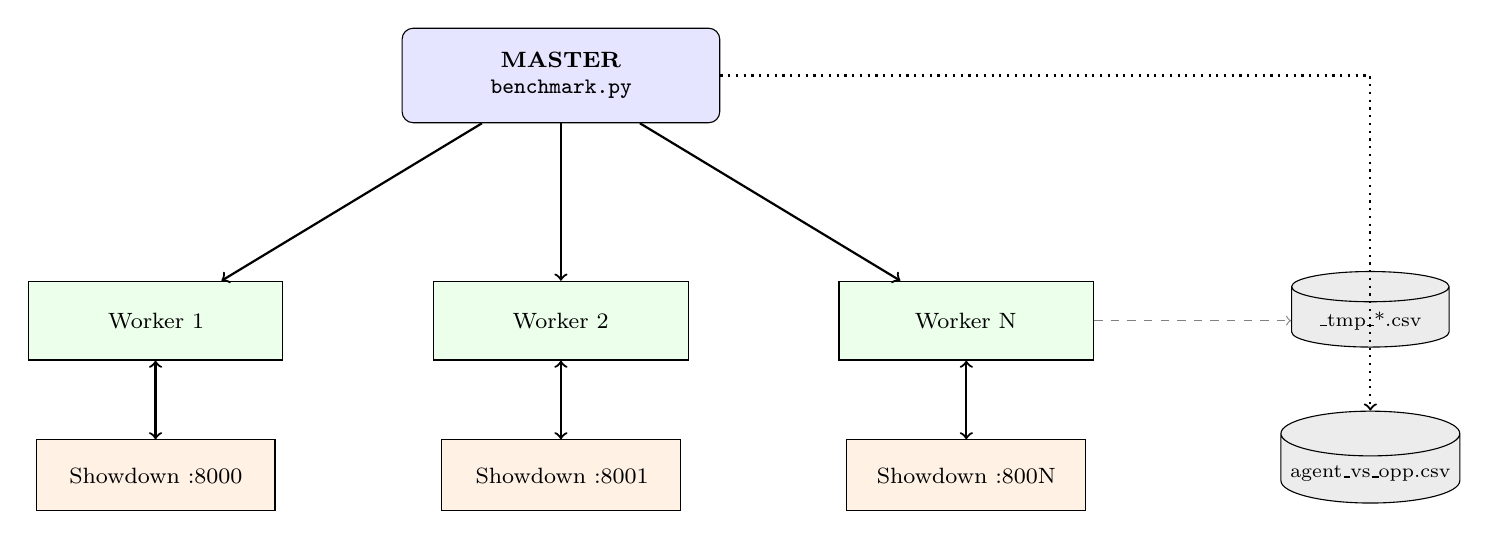
\begin{tikzpicture}[
        node distance=1cm, font=\footnotesize,
        master/.style={rectangle, draw, fill=blue!10, text width=3.8cm, align=center, minimum height=1.2cm, rounded corners},
        worker/.style={rectangle, draw, fill=green!8, text width=3cm, align=center, minimum height=1cm},
        server/.style={rectangle, draw, fill=orange!10, text width=2.8cm, align=center, minimum height=0.9cm},
        disk/.style={cylinder, draw, fill=gray!15, shape border rotate=90, aspect=0.25, minimum height=0.9cm, minimum width=2cm, align=center, font=\scriptsize}
    ]
        \node[master] (master) {\textbf{MASTER}\\\texttt{benchmark.py}};
        \node[worker, below left=2cm and 1.5cm of master] (w1) {Worker 1};
        \node[worker, below=2cm of master] (w2) {Worker 2};
        \node[worker, below right=2cm and 1.5cm of master] (wn) {Worker N};
        \node[server, below=1cm of w1] (s1) {Showdown :8000};
        \node[server, below=1cm of w2] (s2) {Showdown :8001};
        \node[server, below=1cm of wn] (sn) {Showdown :800N};
        \node[disk, right=2.5cm of wn] (tmp) {\_tmp\_*.csv};
        \node[disk, below=0.8cm of tmp] (final) {agent\_vs\_opp.csv};
        \draw[->, thick] (master) -- (w1);
        \draw[->, thick] (master) -- (w2);
        \draw[->, thick] (master) -- (wn);
        \draw[<->, thick] (w1) -- (s1);
        \draw[<->, thick] (w2) -- (s2);
        \draw[<->, thick] (wn) -- (sn);
        \draw[->, dashed, gray] (wn.east) -- (tmp.west);
        \draw[->, thick, dotted] (master.east) -| (final.north);
    \end{tikzpicture}
    \caption{Master--worker del gauntlet. Sense memòria compartida entre workers.}
    \label{fig:master_worker_full}
\end{figure}

\subsection{Resume i chunks}

Si \texttt{v12\_vs\_abyssal.csv} ja té 4.320 files, el master calcula $n_{\mathrm{to\_run}}=10.000-4.320$ i continua. No hi ha flag \texttt{--resume}: la veritat és el CSV. Cada worker juga chunks de 25, escriu, crida \texttt{reset\_battles()} i \texttt{gc.collect()}. Sense això, 10k batalles en un procés superen 2~GB; amb chunks, $\sim$200--400~MB.

Timeouts: el cost varia tres ordres (heurística $\sim$0,01--0,1~s/partida; MCTS $\sim$2--4~s). El timeout de batch és $\max(7200, 40\cdot n_{\mathrm{batch}})$ segons, per no matar un worker d'MCTS viu ni esperar eternament un penjament.

\subsection{Reinici de Showdown}

V8 fragmenta l'\textit{old generation}. Empíricament, després de milers de batalles el procés Node creix de $\sim$80~MB a $>400$~MB i la latència puja. El master fa \texttt{pkill} + relançament cada $N$ matchups actius (\texttt{--restart-every}, defecte 3). Cost $\sim$17~s de downtime, negligible en una nit.

\subsection{Esquema CSV}

Cada fila és una batalla. Identitat (\texttt{battle\_id}, \texttt{format}, \texttt{heuristic}, \texttt{opponent}, \texttt{won}, \texttt{turns}), qualitat de decisió (fallbacks, errors), HP i fainted, canvis voluntaris/forçats, RNG (crit, miss, SE), i telemetria de paradigma (\texttt{search\_diff}, \texttt{xgb\_stays}, \texttt{ko\_guards}, \texttt{terastallized}, \ldots). \texttt{StatsBattle} intercepta \texttt{|-crit|} i companyia abans que poke-env les descarti. Els agents no cal que sàpiguen que existeix.

La Figura~\ref{fig:ram_usage} (de la fase de Singles) mostra el perfil de dents de serra: pujada durant un matchup, caiguda al reinici.

\begin{figure}[H]
    \centering
    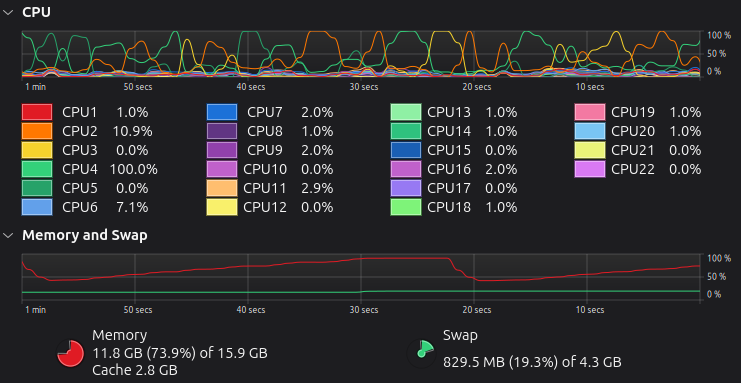
\includegraphics[width=0.85\linewidth]{ram_usage_singles1.png}
    \caption{RAM durant un benchmark de Singles. Les dents de serra són reinicis de Showdown + GC, no un memory leak «resolt» a mà dins el worker.}
    \label{fig:ram_usage}
\end{figure}

\subsection{Contracte \texttt{BaseHeuristic1v1}}

Patró Template Method: \texttt{choose\_move} crida \texttt{\_pre\_move\_hook} (sortida primerenca: KO), \texttt{\_select\_action} (lògica) i, si cal, \texttt{choose\_random\_move} (fallback). Una excepció no gela la batalla: es compta \texttt{error\_moves} i es juga atzar. Tots els agents interns hereten d'aquí, inclosos minimax, MCTS i IL.

\texttt{AgentFactory.create("v20")} és l'únic punt d'instanciació. Baselines: wrappers locals de \texttt{random}, \texttt{max\_power}, \texttt{simple\_heuristic} (còpia amb Tera, perquè el SimpleHeuristics de poke-env no n'havia), \texttt{safe\_one\_step} (reimplementació sense LocalSim per evitar penjades), i \texttt{abyssal} del fork Pokechamp.

% ============================================================
\section{Heurístiques \texttt{v1}--\texttt{v14}: ablació de coneixement}
\label{sec:heur_impl}

L'escala no és «catorze bots cada cop un xic millors». És un experiment: quina peça de coneixement mou el WR a Random Battle. La genealogia de \emph{codi} (Figura conceptual) té branques: \texttt{v1}$\to$\texttt{v2}$\to$\texttt{v3}$\to$\texttt{v6}; \texttt{v4}/\texttt{v5} a part; \texttt{v7} reescriu; \texttt{v8}--\texttt{v14} creixen d'aquest nucli estratègic. \texttt{v14} hereta \texttt{v13}, que hereta l'esperit de \texttt{v12}, no necessàriament el WR.

\paragraph{\texttt{v1}--\texttt{v6} (altiplà de dany).}
\texttt{v1} maximitza $\mathrm{bp}\times\mathrm{eff}\times\mathrm{STAB}$ i gairebé no canvia. \texttt{v2} afegeix stats i cremada. \texttt{v3} tracking de moviments i pivot (Toxic, outspeed). \texttt{v4}/\texttt{v5} clima, terrain, boosts. \texttt{v6} és un \texttt{v3} lleuger amb prioritat. El resultat empíric ---tot el clúster a 44--46\%--- és la tesi d'aquesta fase: més fidelitat a la fórmula de dany no guanya Random Battles.

\paragraph{\texttt{v7} (salt posicional).}
Reescriptura: hazards, setup, pre-check de KO, switch per puntuació de matchup (fórmula d'estil Abyssal). És el primer agent que \emph{tria} canviar, no només desmaia.

\paragraph{\texttt{v8} / \texttt{v10}.}
Meta: items (Life Orb, Choice), habilitats (Levitate, Flash Fire), pantalles, Trick Room. Status (Toxic, Will-O-Wisp, Thunder Wave), sacrifici $\le 20\%$ HP (no gastar un torn per salvar un moribund), U-turn / Volt Switch. Increments reals i petits.

\paragraph{\texttt{v9} / \texttt{v11} (tempo).}
La regla que val més que tota la taula d'objectes de \texttt{v8}: hazards i setup \textbf{només en torn lliure} (outspeed i resist STAB rival). \texttt{v11} híbriditza \texttt{v9}+\texttt{v10} i a penes mou l'agulla.

\paragraph{\texttt{v12} (Gen~9 jugada com a Gen~9).}
Tres peces natives del format:

\begin{enumerate}
    \item Teracristal·lització ofensiva i defensiva.
    \item Lead de \texttt{teampreview}: millor matchup mitjà contra les sis espècies conegudes.
    \item Switch-in després de faint per matchup, no l'slot 0 (ni \texttt{choose\_random\_move}, que és el que fan Abyssal/SimpleHeuristic quan \texttt{active is None}).
\end{enumerate}

A més conserva torns lliures, sack, pivots i KO. Empíricament és el sostre bot-contra-bot.

\paragraph{\texttt{v13}.}
Lazy-load de \texttt{sets.json}: predicció de moviments, item i ability. Matchup amb dany simulat, no només tipus. Choice-lock, phaze vs sweepers, recuperació $<60\%$ HP, Tera conservador (no gastar-lo a $<30\%$ HP ni en un status). Corregeix un fallback de switch-in de \texttt{v12}.

\paragraph{\texttt{v14} (orientat a humans).}
Yomi~2: perfil \texttt{PREDICTIVE} vs \texttt{CONSERVATIVE} segons la taxa de canvis del rival. Scouting als torns 1--3 (Protect, U-turn, Knock Off). 16 rolls de dany per KO garantit. Solver 1-ply d'endgame quan queden $\le 2$ mons per bàndol. Tera defensiu de parany. Contra un bot determinista, scouting i Yomi són sovint \emph{over-respect}: gasten tempo que \texttt{v12} gasta atacant. Això és disseny, no un bug, i el gauntlet ho quantifica.

Tots registren comptadors. \texttt{ko\_checks} explota a $\sim$15/partida a \texttt{v14} perquè el calculador de 16 rolls dispara constantment.

% ============================================================
\section{Minimax 1-ply \texttt{v15}--\texttt{v17}}
\label{sec:mm_impl}

Els tres hereten \texttt{HeuristicV14}. Abans de la matriu: KO garantit (i, a \texttt{v16}/\texttt{v17}, stop de setup, absorb de status, U-turn primerenc). Si no hi ha drecera, s'enumeren les accions pròpies contra les respostes \emph{predites} del rival (moviments revelats, omplerts amb la DB de sets, més un switch hipotètic si el matchup és dolent). Velocitat i prioritat es resolen analíticament: si el ràpid KO, l'acció del lent és nul·la. \textbf{No hi ha \texttt{LocalSim}.}

Fulla de \texttt{v15}: HP i matchup després del torn, amb dany rival $\times 1{,}5$. \texttt{v16} afegeix bonuses de setup / hazard / recuperació / status ($0{,}25$--$0{,}35$) ---la hipòtesi de l'efecte horitzó «s'arregla a la fórmula». \texttt{v17} és \texttt{v16} més $+0{,}15$ al score worst-case de l'acció que hauria triat \texttt{v14}.

Per què no 2-ply: $9\times 9=81$ cel·les a 1-ply, $81^2=6561$ a 2-ply, inassumible amb 16 rolls en Python dins el timer de Showdown. El README del repositori que anomena \texttt{v16} «2-ply» és \textbf{incorrecte}; \texttt{v16} és 1-ply amb fulla posicional.

Telemetria: \texttt{search\_fire\_rate}, \texttt{search\_diff} (override de la sonda \texttt{v14}). Sense aquests camps es podria vendre l'agent com a «minimax cada torn». Amb ells, es veu que la matriu corre en el 16--18\% dels torns.

% ============================================================
\section{IS-MCTS \texttt{v18}--\texttt{v20}}
\label{sec:mcts_impl}

Mateix professor \texttt{v14}, mateix pressupost:

\begin{itemize}
    \item 100 simulacions per torn de cerca, $C=1{,}4$.
    \item Rollout de 5 torns amb \texttt{LocalSim} (Python in-process, fork Pokechamp; no el Node.js per cada pas).
    \item Cada simulació determiniza el rival amb la DB de sets.
    \item Fills arrel: moviments \emph{i} canvis; es juga l'argmax de visites.
\end{itemize}

\texttt{v18}: UCB1, fulla HP/boosts/status/hazards, només KO abans de l'arbre. \texttt{v19}: UCB1, fulla amb rols i amenaça OHKO, i les dreceres tàctiques de \texttt{v14} \emph{abans} de l'arbre. \texttt{v20}: \texttt{v19} + \textbf{PUCT} amb prior $0{,}70$ sobre l'acció \texttt{v14}.

\texttt{LocalSim} $\neq$ Showdown. Un desajust de mecànica és soroll al backup d'UCB1 i una causa plausible de l'override-i-perdre de \texttt{v18}/\texttt{v19}. El minimax 1-ply \textbf{no} usa LocalSim: el seu override-i-perdre no es pot atribuir al simulador, sinó al maximin.

Etiqueta: \texttt{v18}--\texttt{v20} són MCTS, no IL. Documents vells del repositori que diuen el contrari es descarten.

% ============================================================
\section{Imitació \texttt{v21}--\texttt{v22}}
\label{sec:il_impl}

\subsection{Dades}

Replays humans \texttt{gen9randombattle}, Elo $\ge 1800$, HuggingFace / Pokechamp, finestra 2023--2025. $\sim$1,12 milions de torns. \texttt{GroupShuffleSplit} per \texttt{battle\_id}: els torns d'una mateixa batalla no filtren al test. Desbalanceig move/switch $\approx 2{,}88$; \texttt{scale\_pos\_weight} ho compensa.

No és OU. El model antic entrenat en OU i avaluat en Random Battle ($\sim$2\% WR) era un mismatch de format, no una refutació de l'IL.

\subsection{Cap macro}

XGBoost, 1.150 features (HP, hazards, Tera flags, one-hot d'espècie activa, \ldots), $n_{\mathrm{estimators}}=200$, $\mathrm{depth}=6$, $\eta=0{,}1$. Sortida: $p(\mathrm{switch})$. Llindar calibrat $\tau=0{,}5525$ (\texttt{xgboost\_advanced\_threshold.json}). Accuracy de classificació $\sim$65,5\%, ROC-AUC $\sim$0,72: n'hi ha prou per un prior de timing, no per un jugador.

\subsection{Dues piles}

\paragraph{\texttt{v21} (\texttt{HeuristicV21XGBoost}).}
Hereta \texttt{v14}. Ordre: KO garantit $\to$ endgame $\le 2$ mons $\to$ setup/absorb $\to$ XGBoost. Si SWITCH: pivot o \texttt{\_get\_best\_switch} de \texttt{v14}. Si MOVE: \texttt{\_score\_move} de \texttt{v14}. Guard de loop. Empíricament XGB dispara en el 15\% dels torns.

\paragraph{\texttt{v22} (\texttt{HeuristicV22PureIL}).}
Només \texttt{BaseHeuristic1v1}. XGB primer. Switch: puntua cada mons del banc com si fos l'actiu i tria el de $p(\mathrm{switch})$ mínima. Move: segon model \texttt{xgboost\_move\_evaluator.json} (atributs: power, STAB, eff, status, prioritat --- no el nom del moviment). Zero KO guards. Loop guard gairebé sempre.

El README que intercanvia híbrid i pur és \textbf{incorrecte}. \texttt{v21} és l'híbrid; \texttt{v22} és el clon.

% ============================================================
\section{Baselines}

\texttt{random}, \texttt{max\_power}: poke-env. \texttt{simple\_heuristic}: còpia local amb Tera. \texttt{abyssal}: Pokechamp. \texttt{one\_step} i \texttt{safe\_one\_step} apunten al player matemàtic sense LocalSim. Abyssal i Simple Heuristic són, en aquest gauntlet, gairebé el mateix rival (Elo 1755 tots dos, empatats amb \texttt{v14}).

% ============================================================
\section{Bot en línia}

\texttt{run\_online\_bot.py} connecta qualsevol etiqueta de l'\texttt{AgentFactory} al servidor públic. Mode \texttt{ladder} o \texttt{accept}. La mostra de tesi és \texttt{v14}, usuari \texttt{SirPThesis}, 9--10 de juny de 2026, 431 partides. No s'ha fet un ladder de \texttt{v12}: el protocol bot-contra-bot i el protocol humà es queden separats.

% ============================================================
\section{PPO (framework, no experiment d'aquesta memòria)}
\label{sec:ppo_impl}

\texttt{src/p05\_ppo\_drl/} encapsula un \texttt{PokemonMaskedEnv} (accions 0--3 moviments, 4--9 switches), vectorització, MaskablePPO~\cite{sb3_contrib} i un currículum Random $\to$ MaxPower $\to$ SimpleHeuristic $\to$ gauntlet. Això documenta que el cinquè paradigma \emph{es pot} entrenar sobre el mateix Showdown. \textbf{No s'hi reporta cap WR.} La comparació prevista és vs \texttt{v12}, a part, no una fila més de la matriu 28.

% !TEX root = ../main.tex
\chapter{Resultats}
\label{chap:resultats}

Aquest capítol llegeix els artefactes del Capítol~\ref{chap:implementacio} sota el protocol del Capítol~\ref{chap:metodologia}. No es reobren el POSG, l'ablació ni el motor: aquí es mesura. Tres ancoratges es donen per fixats: \texttt{v12} és el millor resultat \emph{observat} a la matriu; \texttt{v14} és l'heurística de \emph{servei} (fulla, prior, executor i bot de \emph{ladder}), no el sostre de rendiment; MaskablePPO s'avalua fora de la matriu, contra \texttt{v12}.

Les fonts internes són els 784 CSV de \path{data/benchmarks/all_10k/gen9randombattle} ---\textbf{6.409.000} partides dirigides---, produïts pel pipeline de la Secció~\ref{sec:reporting_impl} (\texttt{generate\_heatmap.py}, \texttt{elo\_ranking.py}, informes a \path{src/p00_core/reporting/agents/}) i \path{src/p05_ppo_drl/RESULTS.md}. Un \textbf{resultat observat} és una taxa o un comptador; una \textbf{interpretació} relaciona indicadors amb el disseny; una \textbf{hipòtesi explicativa} requeriria una ablació nova per confirmar-se.

% ============================================================
\section{Protocol de lectura dels resultats}
\label{sec:res_protocol}

28 agents, cadascun com a \emph{nosaltres} contra 28 oponents, format \texttt{gen9randombattle}, estructurats segons la taxonomia de la Taula~\ref{tab:taxonomy}. Fitxers dirigits \texttt{A\_vs\_B.csv}. PPO es llegeix a part (Secció~\ref{sec:res_ppo}).

\begin{table}[H]
\centering
\caption{Taxonomia dels 28 agents del gauntlet \texttt{gen9randombattle}. Els identificadors es mantenen en anglès. El prefix de la figura de calor indica el paradigma: (H)~heurística, (MM)~minimax, (MCT)~MCTS, (IL)~imitació, (B)~baseline.}
\label{tab:taxonomy}
\small
\begin{tabular}{llp{8.2cm}}
\toprule
\textbf{IDs} & \textbf{Paradigma} & \textbf{Què és, en una frase} \\
\midrule
\texttt{random}, \texttt{max\_power}, \texttt{one\_step}, \texttt{safe\_one\_step}, \texttt{abyssal}, \texttt{simple\_heuristic}
  & Baselines (B)
  & Referents de \textit{poke-env} i d'estil Pokechamp: atzar, potència bruta, un pas de dany, i heurístiques de matchup. \\
\texttt{v1}--\texttt{v14}
  & Heurístiques (H)
  & Escala d'ablació per construcció: cada versió afegeix una peça de coneixement expert (dany, hazards, Tera, Yomi,\ldots). \\
\texttt{v15}--\texttt{v17}
  & Minimax 1-ply (MM)
  & Maximin analític d'un torn sobre \texttt{HeuristicV14}; sense \texttt{LocalSim}. \\
\texttt{v18}--\texttt{v20}
  & IS-MCTS (MCT)
  & 100 simulacions $\times$ 5 torns de \texttt{LocalSim}; cel·les amb $n=1.000$. \\
\texttt{v21}
  & IL híbrid (IL)
  & Macro XGBoost (mou vs canvia) + execució \texttt{v14}. \\
\texttt{v22}
  & IL pur (IL)
  & El mateix macro, dos XGBoost, \textbf{sense} \texttt{v14}. \\
\texttt{v23+}
  & PPO (fora del gauntlet)
  & Framework a \texttt{src/p05\_ppo\_drl/}; no forma part d'aquesta matriu. \\
\bottomrule
\end{tabular}
\end{table}


La fila és l'agent analitzat i la columna, l'oponent. Un 59,91 a la cel·la \texttt{v12} $\times$ Abyssal indica 5.991 victòries de 10.000 en aquell fitxer dirigit.

Cada cel·la és una proporció binomial. Els intervals són Wilson al 95\% (Equació~\ref{eq:wilson_ci}); els tres pisos mostrals són els de la Taula~\ref{tab:ci_n}. A $n=10.000$ el marge màxim d'una taxa individual és de $\pm 0{,}98$~pp; a $n=1.000$ (totes les cel·les MCTS), $\pm 3{,}10$~pp. La Pokédex no entra a $\mathrm{Var}(\hat p)$: s'estima una taxa marginal sota el generador d'equips de la Generació~IX.

Per a la comparació entre dues condicions o agents independents, s'aplica el contrast de dues proporcions (Equacions~\ref{eq:se_diff}--\ref{eq:ci_diff}): a $n=10.000$, la diferència mínima detectable per a una significança estadística al nivell $\alpha=0{,}05$ és de $|\Delta \hat{p}| \ge 1{,}39$~pp ($z \ge 1{,}96$, tercera columna de la Taula~\ref{tab:ci_n}); a $n=1.000$, el llindar és de $|\Delta \hat{p}| \ge 4{,}38$~pp. Les diferències inferiors a aquests llindars es troben dins el marge d'error conjunt i es consideren empats tècnics o variacions no significatives que no admeten interpretació de superioritat.

\begin{itemize}
    \item Fila no MCTS: \textbf{253.000} partides ($25\times 10.000$ i $3\times 1.000$ contra MCTS).
    \item Fila MCTS: \textbf{28.000} partides ($28\times 1.000$).
    \item Matriu: \textbf{6.409.000} partides dirigides. Les orientacions recíproques sumen $\approx 100\%$ i l'autojoc se situa prop del 50\%.
\end{itemize}

La taxa global d'una fila no MCTS pondera els oponents MCTS deu vegades menys; en una fila MCTS tots pesen igual. La comparació entre paradigmes es basa en cel·les comunes ---especialment contra \texttt{v12}---, no en una única ordenació global. Les proves de desenvolupament amb 100 partides no entren a les conclusions.

% ============================================================
\section{Controls globals de la matriu}
\label{sec:res_controls}

Abans d'interpretar versions concretes, es comproven la cobertura, la distribució de taxes i la durada de les batalles sobre les 784 cel·les dirigides:
\begin{itemize}
    \item \textbf{Cobertura:} La reducció mostral segueix estrictament el paradigma (10.000 partides per cel·la al bloc general i 1.000 a MCTS pel cost computacional de les simulacions), assegurant la consistència del banc d'avaluació.
    \item \textbf{Distribució de taxes:} La taxa de victòries es concentra al voltant del 50\% (autojoc i duels equilibrats) amb acumulacions als extrems (0\% i 100\%) degudes a referències febles (\texttt{random}, \texttt{max\_power}). Per aquest motiu, la taxa global no s'interpreta com una habilitat absoluta: millorar contra oponents febles té un valor discriminant molt limitat.
\end{itemize}

\begin{figure}[htbp]
    \centering
    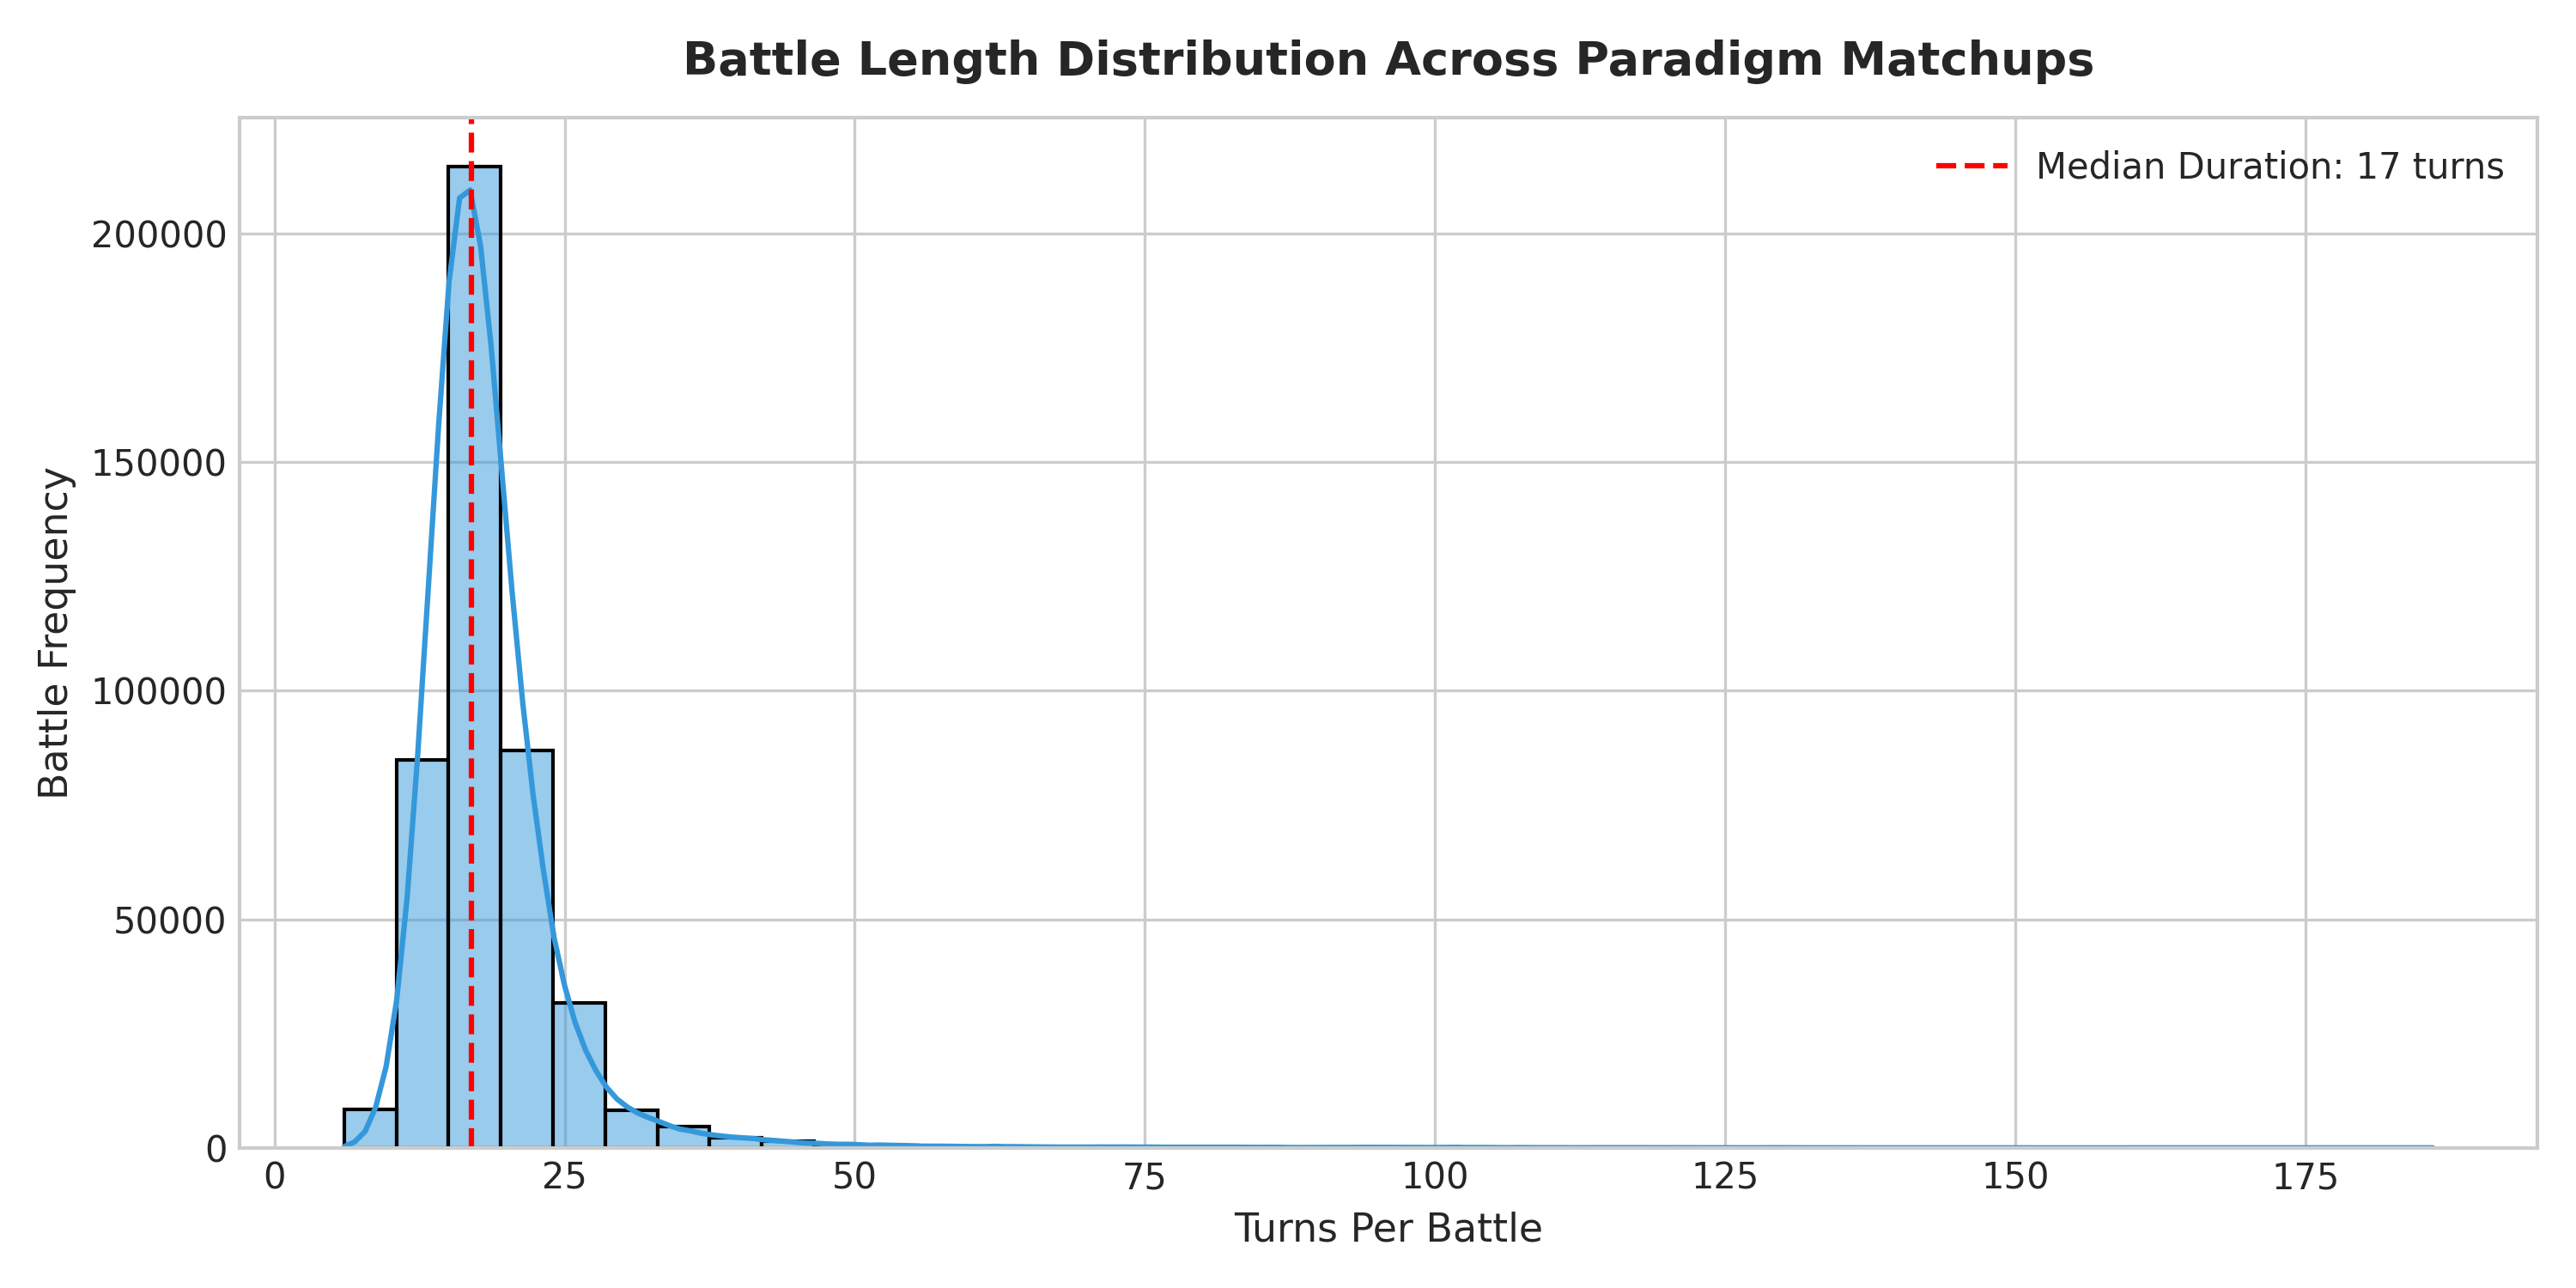
\includegraphics[width=0.88\linewidth]{images/results/game_length_distribution.png}
    \caption{Distribució de la durada de les batalles analitzades. La mediana és de 17 torns i hi ha una cua dreta de partides excepcionalment llargues.}
    \label{fig:length_distribution}
\end{figure}

Pel que fa a la durada (Figura~\ref{fig:length_distribution}), la mediana se situa clarament en 17 torns (amb el gruix entre 10 i 25 torns) i presenta una cua dreta per atrició defensiva o bucles de canvis. Com que dues polítiques poden assolir una mateixa taxa tancant ràpidament o bé dilatant el combat per conservació de recursos, les anàlisis posteriors combinen sempre torns, supervivents finals i motiu dels canvis.

% ============================================================
\section{Fil conductor de \texttt{v1} a \texttt{v22}}
\label{sec:version_timeline}

La Taula~\ref{tab:version_timeline} resumeix la seqüència abans d'analitzar-la. Les taxes globals són descriptives i no fan comparable l'MCTS amb la resta a causa de la ponderació diferent; la seva funció aquí és mostrar els canvis de règim.

\begin{table}[htbp]
\centering
\caption{Evolució de les preguntes i dels resultats entre \texttt{v1} i \texttt{v22}.}
\label{tab:version_timeline}
\small
\begin{tabularx}{\textwidth}{lXrX}
\toprule
\textbf{Versions} & \textbf{Pregunta que materialitzen} & \textbf{TV global} & \textbf{Patró observat} \\
\midrule
\texttt{v1}--\texttt{v6} & Fins on arriba refinar dany i ordre immediat? & 44--46\% & Altiplà; telemetria gairebé invariable. \\
\texttt{v7}, \texttt{v8}, \texttt{v10} & Què aporta valorar la posició i canviar? & 54--56\% & Salt a \texttt{v7}; afegits posteriors petits. \\
\texttt{v9}, \texttt{v11} & Preparació i perills només en torns segurs? & 59\% & Nou augment i aparició dels comptadors de ritme. \\
\texttt{v12} & Què aporten Tera i el substitut informat? & 69,01\% & Increment més gran i 59,91\% contra Abyssal. \\
\texttt{v13}, \texttt{v14} & Més inferència i model del rival sempre ajuden? & 67,63 / 62,03\% & Inversió: més complexitat, menys taxa global. \\
\texttt{v15}--\texttt{v17} & Un maximin d'un torn corregeix \texttt{v14}? & 53,80--57,89\% & La variant guiada discrepa menys i és la millor. \\
\texttt{v18}--\texttt{v20} & Cinc torns simulats superen l'horitzó curt? & 53,29--59,66\% & PUCT millora UCB1, però no supera \texttt{v12}. \\
\texttt{v21}, \texttt{v22} & Es pot imitar quan atacar o canviar? & 58,71 / 33,49\% & L'executor heurístic és determinant. \\
\bottomrule
\end{tabularx}
\end{table}

La primera meitat de la seqüència acumula coneixement explícit fins a \texttt{v12}. La segona canvia de paradigma, però la majoria de decisions encara passen per dreceres o priors derivats de \texttt{v14}. El patró general no és «algorisme més sofisticat, agent més fort», sinó «representació i coneixement adequats, seguits d'un mòdul que no els destrueixi».

PPO no rep un número \texttt{v23} ni forma part de la taula global. La seva pregunta és paral·lela: si una política neuronal inicialitzada amb \texttt{v8} pot arribar a \texttt{v12}. El resultat de 34,1\% contra aquest comparador es tracta a la Secció~\ref{sec:res_ppo}.

% ============================================================
\section{L'escala heurística: tres canvis de règim}
\label{sec:res_heur}

\begin{table}[H]
\centering
\caption[Seqüència heurística \texttt{v1}--\texttt{v14}.]{Seqüència heurística \texttt{v1}--\texttt{v14} (253.000 partides per fila). La taxa global no creix de manera monotònica: els increments principals apareixen a \texttt{v7}, \texttt{v9} i \texttt{v12}, i les dues versions posteriors disminueixen.}
\label{tab:heur_ladder}
\small
\begin{tabularx}{\textwidth}{llrr>{\raggedright\arraybackslash}X}
\toprule
\textbf{Agent} & \textbf{Règim} & \textbf{TV (\%)} & \textbf{contra Abyssal} & \textbf{Incorporació principal} \\
\midrule
\texttt{v1}--\texttt{v6} & Altiplà & 44,25--45,86 & 30,6--32,5 & Dany, clima, modificadors i canvis simples \\
\texttt{v7} & Posicional & 54,25 & 40,80 & Dany modificat i canvi segons l'enfrontament \\
\texttt{v8} & Posicional & 55,43 & 42,30 & Objectes, habilitats, pantalles, Trick Room \\
\texttt{v9} & Ritme segur & 58,86 & 46,64 & Perills i preparació \emph{només en torns lliures} \\
\texttt{v10} & Posicional & 55,66 & 41,86 & Status, sacrifici $\le 20\%$ HP, U-turn \\
\texttt{v11} & Ritme segur & 59,26 & 47,50 & Combinació de \texttt{v9} i \texttt{v10} \\
\texttt{v12} & Mecànica Gen.~IX & \textbf{69,01} & \textbf{59,91} & Tera i selecció del substitut \\
\texttt{v13} & Moviments revelats & 67,63 & 55,34 & Enfrontament amb moviments revelats i Tera conservador \\
\texttt{v14} & Model de rival & 62,03 & 51,36 & Perfil, sondeig inicial, rang de dany i final d'un torn \\
\bottomrule
\end{tabularx}
\end{table}


La Taula~\ref{tab:heur_ladder} i la Figura~\ref{fig:heur_overall_wr} sintetitzen l'evolució de la taxa de victòries global al llarg de la seqüència heurística \texttt{v1}--\texttt{v14}.

\begin{figure}[htbp]
    \centering
    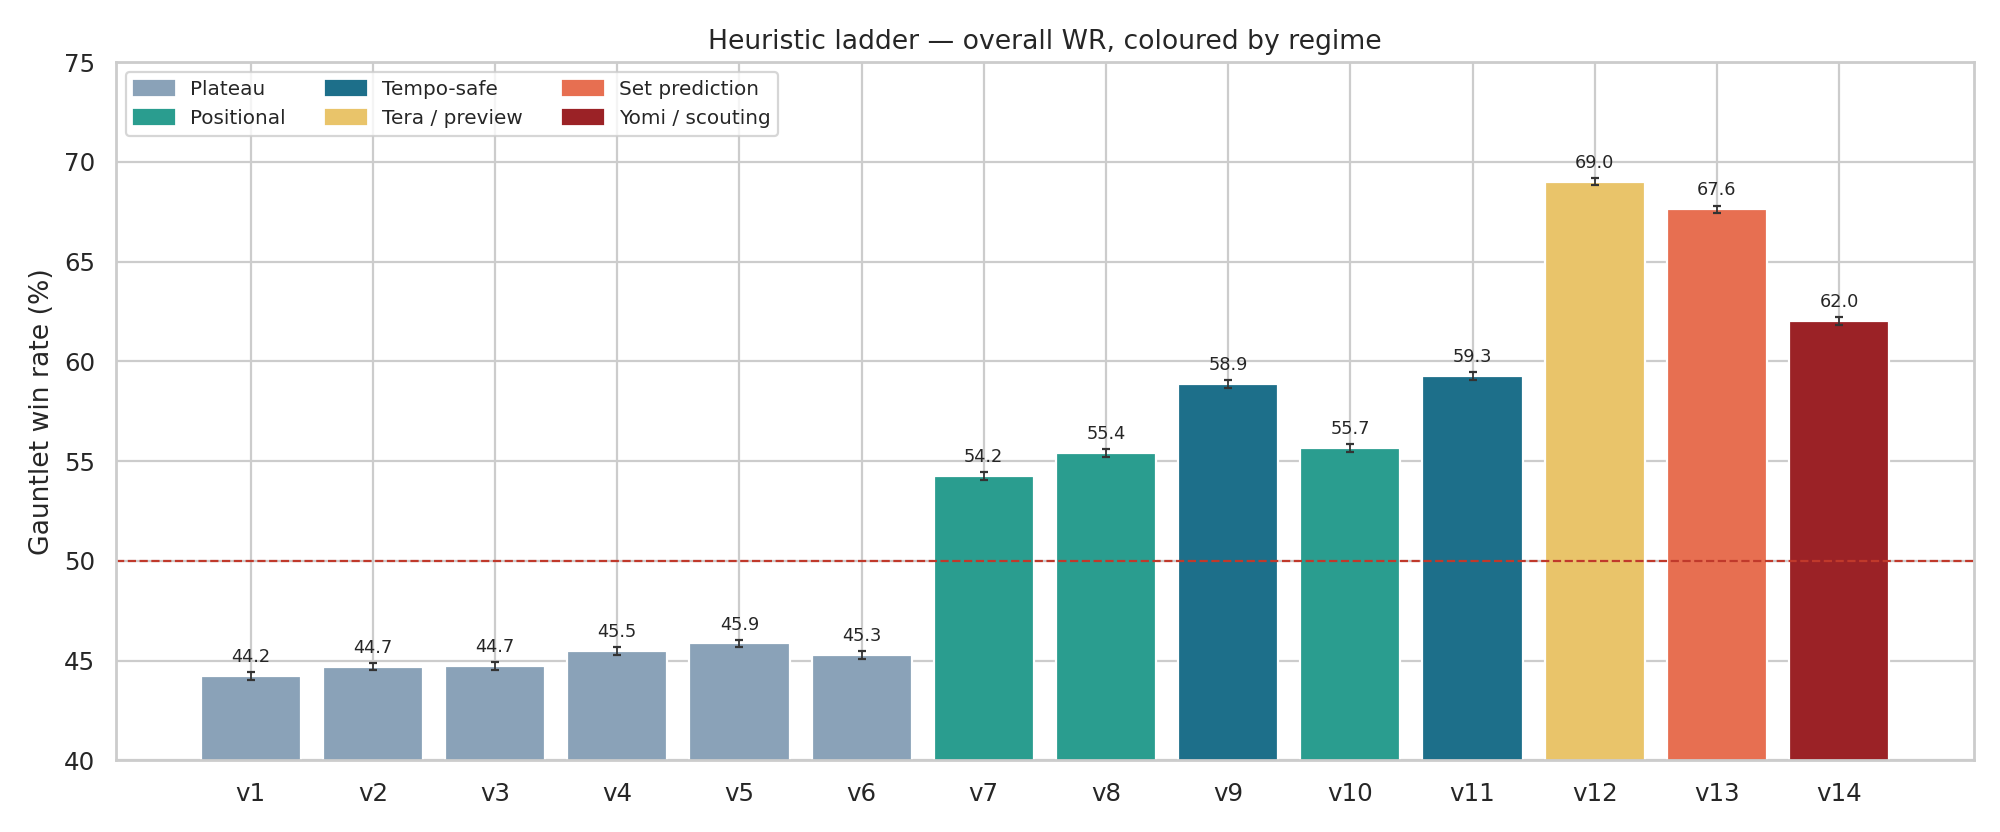
\includegraphics[width=0.95\linewidth]{images/heuristics/heur_overall_wr.png}
    \caption{Taxa global de victòries de \texttt{v1}--\texttt{v14} (253.000 partides per fila; les tres cel·les contra MCTS tenen $n=1.000$). S'observen canvis destacats a \texttt{v7}, \texttt{v9} i \texttt{v12}, seguits d'una disminució a \texttt{v13} i \texttt{v14}.}
    \label{fig:heur_overall_wr}
\end{figure}

\subsection{Altiplà \texttt{v1}--\texttt{v6}: rendiments decreixents del càlcul de dany}

La taxa global recorre \textbf{1,61~pp} (44,25--45,86\%). Els enfrontaments interns se situen prop del 50\%, mentre que contra Abyssal obtenen entre el 30,6\% i el 32,5\%.

En aquestes versions, afinar la fórmula de dany després d'incorporar efectivitat i STAB mostra rendiments decreixents. Els increments posteriors apareixen quan s'afegeixen decisions posicionals i recursos específics del format.

En el conjunt de la matriu (253.000 partides per fila; mitjanes ponderades per nombre de partides), registren aproximadament 1,02 canvis voluntaris per partida, cap Teracristal·lització i uns 4,6 recursos de reserva. Aquest perfil correspon a una política principalment ofensiva amb poca gestió posicional.

\subsection{Primer salt: \texttt{v7} (i \texttt{v8}/\texttt{v10})}

\texttt{v7} incorpora dany amb modificadors i canvis segons l'enfrontament. La taxa global passa d'aproximadament 45,5\% a \textbf{54,25\%}; contra Abyssal, d'aproximadament 32\% a \textbf{40,8\%}.

\texttt{v8} (KO de prioritat conservador i immunitats d'habilitat ja revelades) afegeix 1,2~pp. \texttt{v10} (estats, sacrificis i moviments de pivot) obté una taxa similar a \texttt{v8} (55,66\% i 55,43\%).

La telemetria també canvia: els canvis voluntaris pugen a 1,47 per partida, \texttt{matchup\_switches} arriba a 0,41 i les accions de reserva baixen d'aproximadament 4,6 a 2,18. L'agent passa a seleccionar canvis de manera explícita.

Els perills d'entrada i els moviments de preparació s'incorporen a \texttt{v9}; els comptadors \texttt{setup\_uses} i \texttt{hazard\_sets} deixen de ser zero.

\subsection{Segon salt: \texttt{v9} / \texttt{v11}}

Amb \texttt{v9}, els perills d'entrada i els moviments de preparació només s'utilitzen quan l'agent és més ràpid i resisteix l'STAB rival. La taxa global puja a \textbf{58,86\%} i el resultat contra Abyssal a \textbf{46,64\%}. \texttt{v11} combina aquest bloc amb \texttt{v10} i afegeix 0,4~pp; la contribució addicional és petita en aquesta matriu.

\texttt{v9}/\texttt{v11} són els primers amb aproximadament 1,6 moviments de preparació i 0,16 perills d'entrada per partida.

\subsection{Tercer salt: \texttt{v12}}

\texttt{v12} combina la Teracristal·lització i la selecció informada del substitut després d'un debilitament. La taxa global assoleix el \textbf{69,01\%}, suposant el major increment de tota la seqüència ($+9{,}75$~pp respecte al $59{,}26\%$ de \texttt{v11}). És, a més, el primer agent intern que supera amb claredat Abyssal i Simple Heuristic: \textbf{59,91\%} i \textbf{59,75\%}, respectivament ($n=10.000$, tal com s'il·lustra a la Figura~\ref{fig:heur_vs_baselines} enfront dels comparadors discriminants).

En la telemetria de matriu (recollida en l'empremta tàctica de la Figura~\ref{fig:heur_fingerprint}), utilitza la Teracristal·lització \textbf{0,96 vegades per partida}, registra només \textbf{0,01} accions de reserva i conserva \textbf{1,84} Pokémon, davant d'1,44 a \texttt{v11}. El canvi de comportament és substancial.

Tot i que totes dues millores s'introdueixen conjuntament en aquesta versió, la telemetria granular de la matriu permet desacoblar observacionalment la contribució relativa de cada mecanisme:
\begin{enumerate}
    \item \textbf{Impacte de la selecció del substitut (eliminació de \emph{fallbacks}):} A les versions prèvies (\texttt{v1}--\texttt{v11}), la manca d'un gestor per als torns forçats per debilitament feia que l'agent invoqués el mecanisme per defecte (\texttt{fallback\_moves\_us}), seleccionant el substitut d'entrada uniformement a l'atzar. A \texttt{v12}, la resolució per aparellament (\texttt{\_get\_best\_switch}) redueix les accions de reserva de $\sim 3{,}5$ a pràcticament zero ($0{,}01$ per partida), evitant que l'agent regali la iniciativa entrant en desavantatge elemental greu.
    \item \textbf{Impacte de la Teracristal·lització (el contrast natural amb \texttt{v13}):} A la versió immediatament posterior (\texttt{v13}), la selecció informada del substitut es manté intacta, però l'ús de la Teracristal·lització es restringeix dràsticament, caient un \textbf{79\%} (de $0{,}96$ usos per partida a \texttt{v12} a només $0{,}20$ a \texttt{v13}). Malgrat aquesta reducció massiva de la Tera, el rendiment global només retrocedeix $\approx 1{,}4$~pp (de $69{,}01\%$ a $67{,}63\%$), el duel directe entre totes dues queda en empat virtual ($50{,}65\%$ vs $48{,}85\%$, separat per només $1{,}8$~pp, Taula~\ref{tab:heur_h2h}; el test de proporció respecte al 50\% d'equilibri llança $z = 1{,}30$, $p = 0{,}19$ per a \texttt{v12}, confirmant que la desviació respecte a la paritat és estadísticament no significativa) i \texttt{v13} fins i tot supera \texttt{v12} enfront de la cerca i la imitació (Taula~\ref{tab:v13_vs_search}).
\end{enumerate}

Aquest contrast observacional suggereix com a hipòtesi que el gruix principal del salt ($\approx 7$--$8$~pp) s'atribueix a l'eliminació dels canvis forçats atzarosos i a l'estabilització del posicionament tàctic, mentre que la Teracristal·lització afegeix un marge incremental d'aproximadament $\approx 1{,}4$~pp gràcies a la bonificació de dany elemental i la flexibilitat defensiva.

\begin{figure}[htbp]
    \centering
    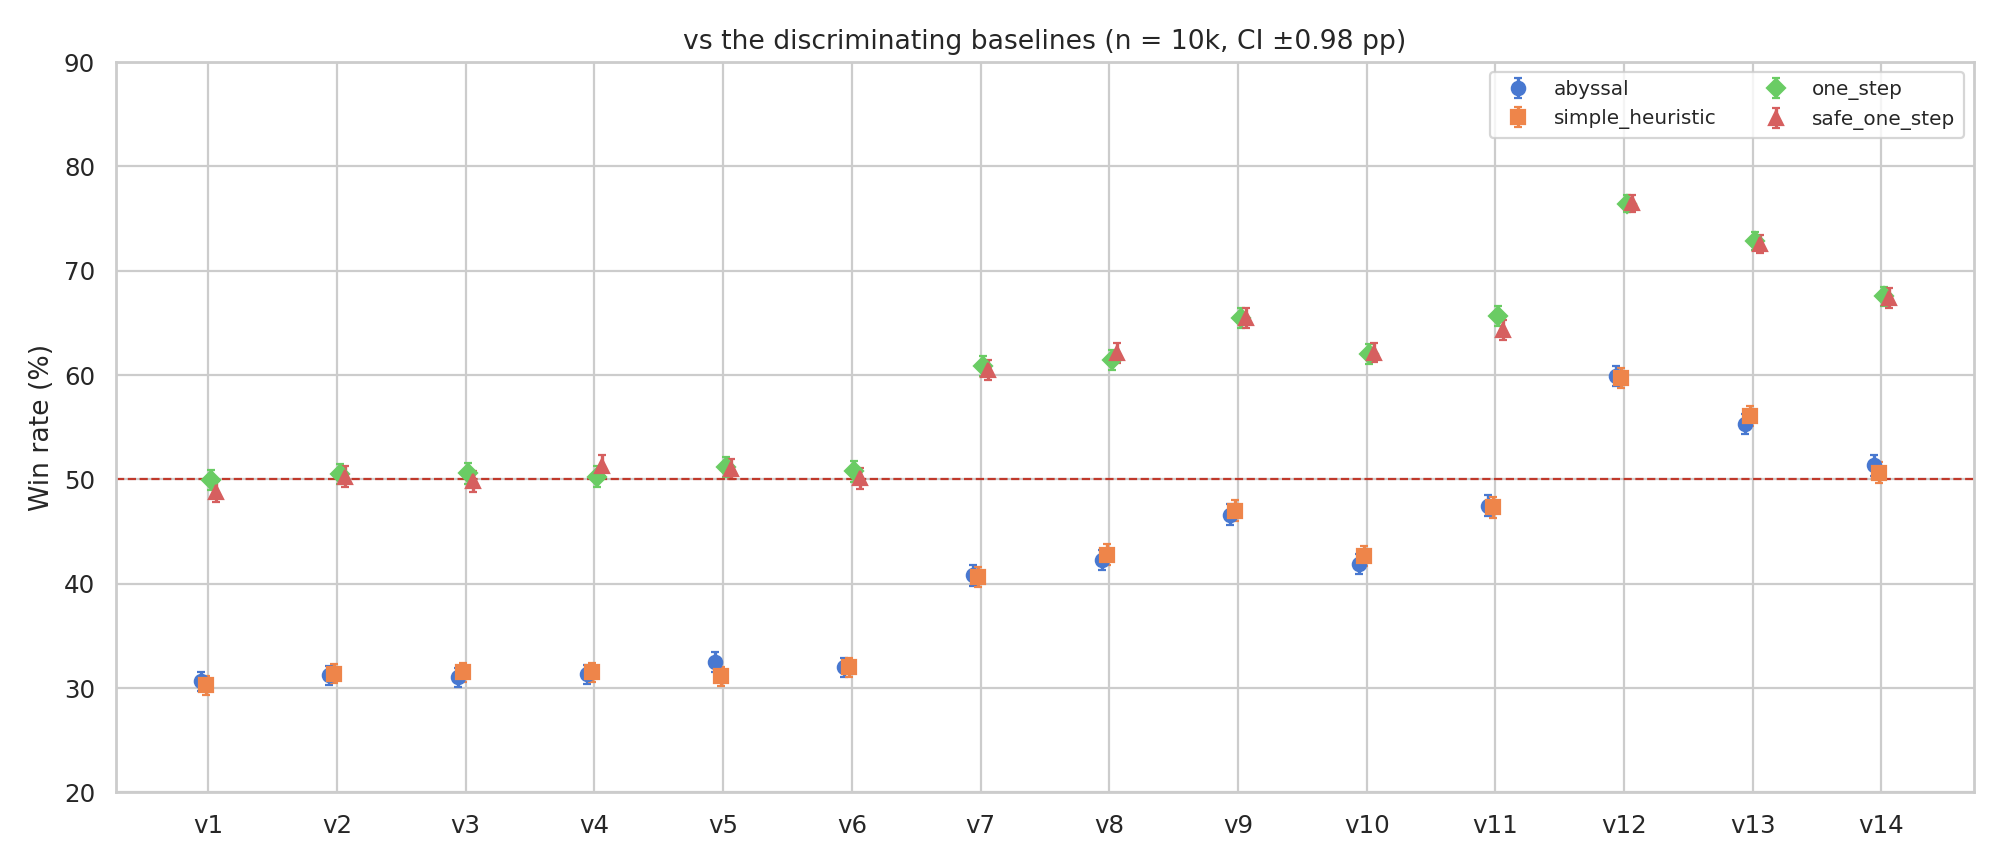
\includegraphics[width=0.95\linewidth]{images/heuristics/heur_vs_baselines.png}
    \caption{\texttt{v1}--\texttt{v14} contra els quatre agents de referència discriminants ($n=10.000$ per cel·la): Abyssal, Simple Heuristic, \texttt{one\_step} i \texttt{safe\_one\_step}. \texttt{v12} és el primer que deixa Abyssal i Simple Heuristic clarament per sota del 50\%. Random i MaxBasePower s'ometen: contra Random totes les heurístiques arriben al 97--98\% i la columna no discrimina.}
    \label{fig:heur_vs_baselines}
\end{figure}

\begin{figure}[htbp]
    \centering
    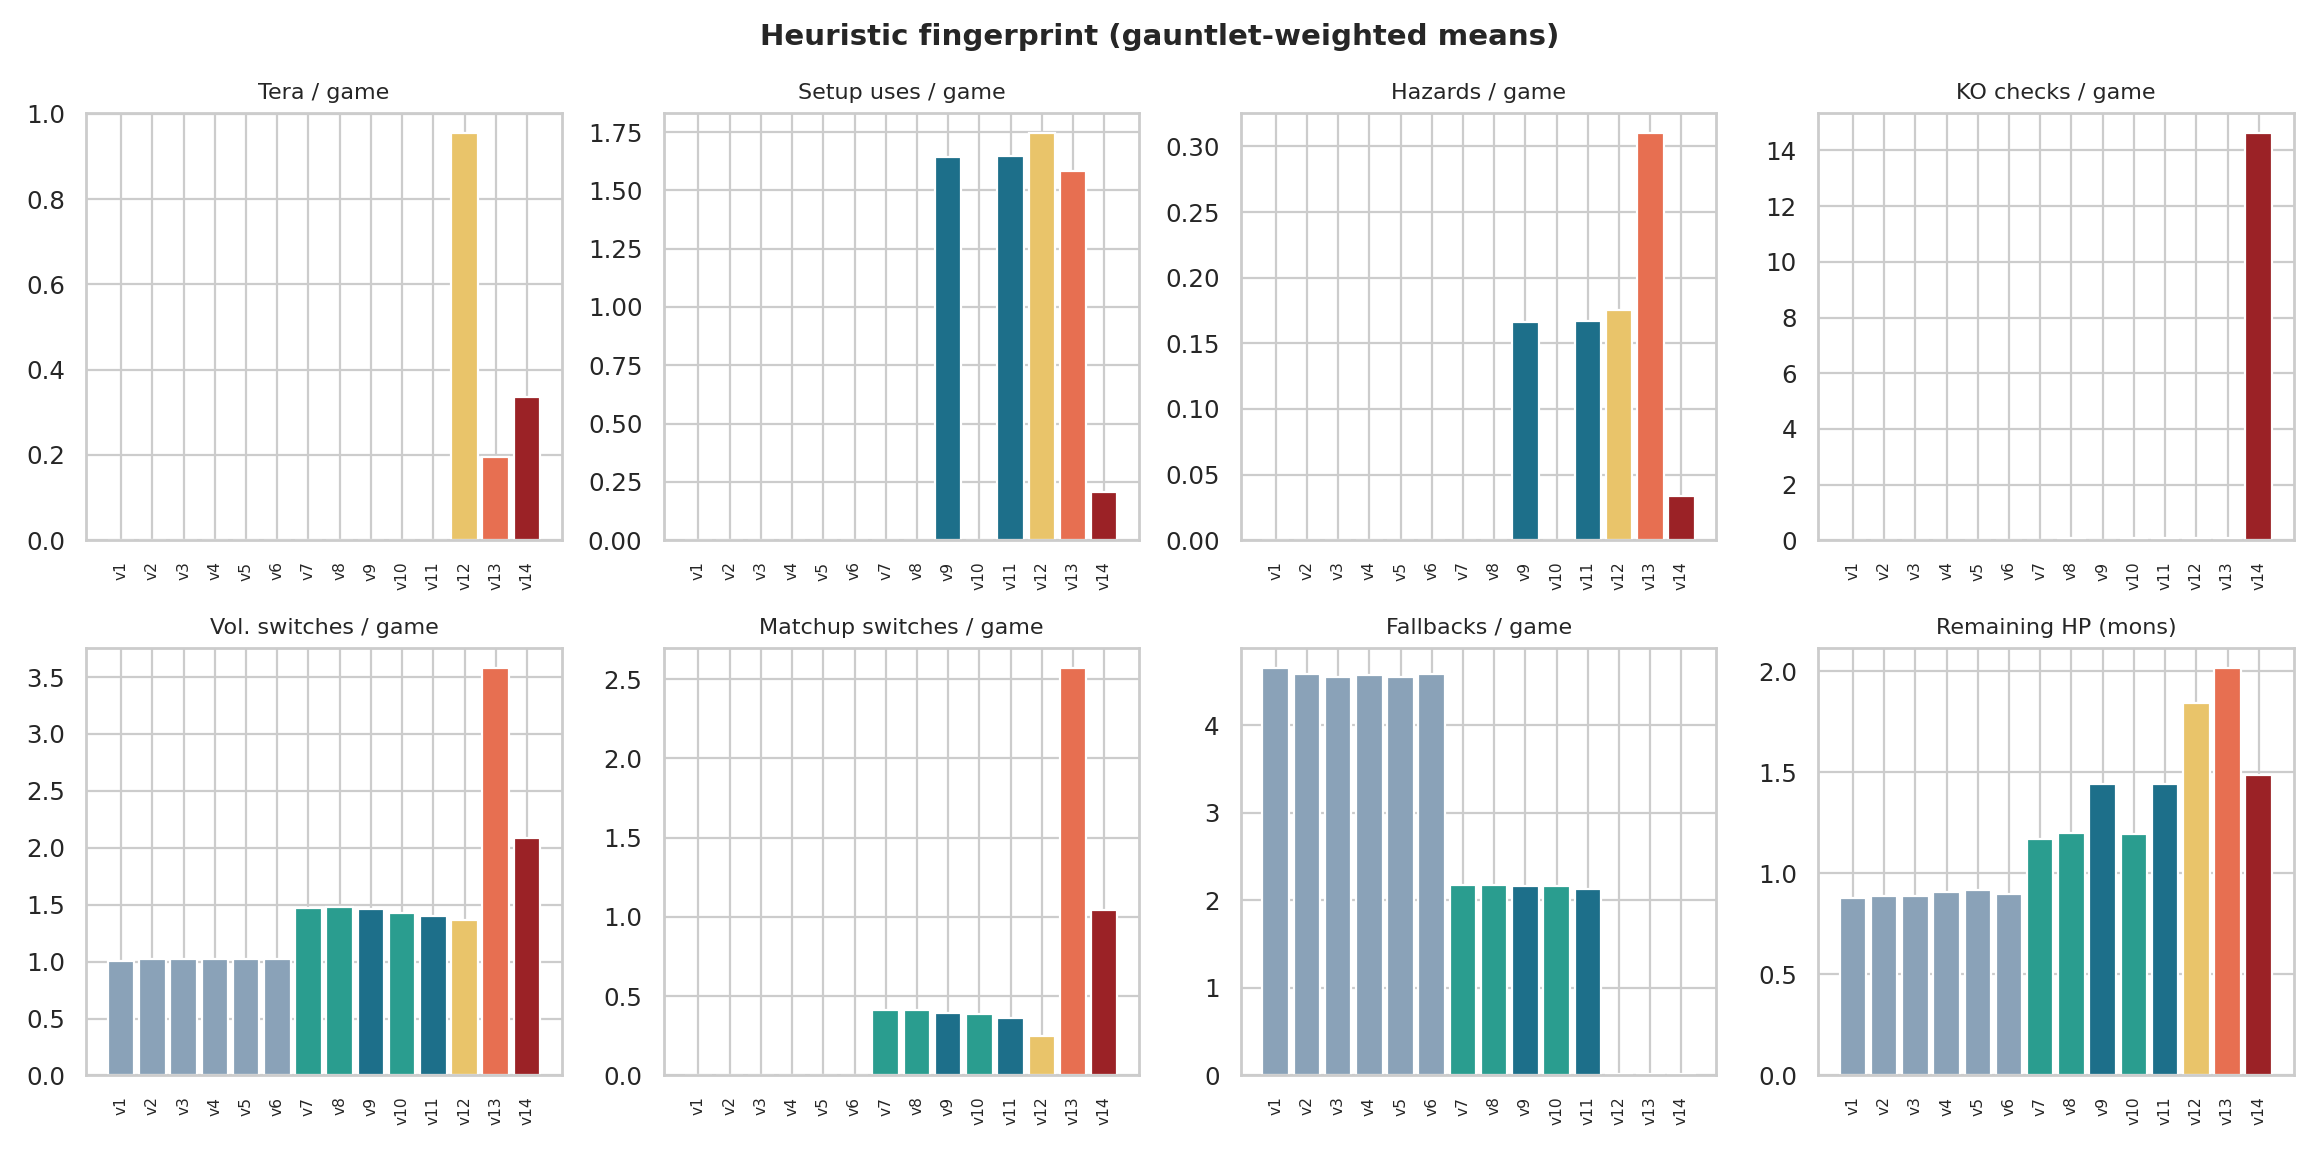
\includegraphics[width=0.95\linewidth]{images/heuristics/heur_fingerprint_bars.png}
    \caption{Empremta tàctica de la seqüència heurística (mitjanes ponderades de la matriu). \texttt{v12} utilitza la Teracristal·lització gairebé una vegada per partida; \texttt{v13}, 0,20 vegades. \texttt{ko\_checks} augmenta fins a aproximadament 15 a \texttt{v14}; la preparació i els perills d'entrada apareixen a partir de \texttt{v9}.}
    \label{fig:heur_fingerprint}
\end{figure}

% ============================================================
\FloatBarrier
\section{La inversió entre \texttt{v12}, \texttt{v13} i \texttt{v14}}
\label{sec:res_inversion}

La complexitat creix de \texttt{v12} a \texttt{v14}, però la taxa global observada disminueix. Aquest resultat mostra que l'herència de funcionalitats no implica una millora monotònica.

\begin{table}[H]
\centering
\caption{Cara a cara de la inversió, $n=10.000$ partides independents cada sentit. \texttt{v12} vs \texttt{v13} és un llançament de moneda (buit de 1,8~pp, cada IC $\pm 0{,}98$). \texttt{v14} perd clarament contra tots dos. Les sumes recíproques $\approx 100\%$ descarten un artefacte de seient.}
\label{tab:heur_h2h}
\small
\begin{tabular}{lrrr}
\toprule
\textbf{Fitxer} & \textbf{WR (\%)} & \textbf{Recíproc (\%)} & \textbf{Suma} \\
\midrule
\texttt{v12\_vs\_v13} & 50,65 & 48,85 & 99,50 \\
\texttt{v12\_vs\_v14} & 56,01 & 44,74 & 100,75 \\
\texttt{v13\_vs\_v14} & 57,71 & 41,60 & 99,31 \\
\bottomrule
\end{tabular}
\end{table}


Tal com reflecteix la Taula~\ref{tab:heur_h2h}, les dues orientacions de \texttt{v12} i \texttt{v13} difereixen només en 1,8~pp (50,65\% i 48,85\%) i no aporten una separació concloent (enfront de la paritat del 50\%, $z = 1{,}30$, $p = 0{,}19$ a l'orientació directa i $z = 2{,}30$, $p = 0{,}02$ a la recíproca; la taxa combinada de les 20.000 partides és del 50,90\%, situant la desviació en un marge pràcticament negligible de $<1$~pp). En canvi, \texttt{v14} queda clarament per sota de tots dos en els enfrontaments directes de manera estadísticament inequívoca (44,74\% davant \texttt{v12}, $z = 10{,}52$, $p < 10^{-15}$, i 41,60\% davant \texttt{v13}, $z = 16{,}80$, $p < 10^{-15}$).

\subsection{On \texttt{v13} encara guanya}

No està estrictament dominat. És el \textbf{millor heurístic contra cerca i contra l'IL híbrid}:

\begin{table}[htbp]
\centering
\small
\caption{Rendiment comparatiu de \texttt{v12}, \texttt{v13} i \texttt{v14} contra cerca, imitació i blocs de control (taxa de victòries en \%).}
\label{tab:v13_vs_search}
\begin{tabular}{lrrr}
\toprule
Oponent & \texttt{v12} & \texttt{v13} & \texttt{v14} \\
\midrule
Minimax \texttt{v15} & 63,96 & \textbf{67,59} & 60,07 \\
Minimax \texttt{v17} & 60,37 & \textbf{64,12} & 56,70 \\
MCTS \texttt{v18} ($n=1$k) & 66,1 & \textbf{67,7} & 59,8 \\
IL \texttt{v21} & 59,12 & \textbf{62,46} & 54,74 \\
Baselines (bloc) & \textbf{76,91} & 74,36 & 71,06 \\
Altres heurístiques (bloc) & \textbf{67,01} & 64,71 & 58,58 \\
\bottomrule
\end{tabular}
\end{table}

\subsection{Per què no supera \texttt{v12} en global}

En la telemetria de matriu, \texttt{v13} utilitza la Teracristal·lització 0,20 vegades per partida, davant de 0,96 a \texttt{v12}; també fa notablement més canvis voluntaris (3,58 davant d'1,37 a \texttt{v12}) i més canvis per enfrontament (2,57 davant de 0,25). Aquest comportament preserva més membres de l'equip al final de la batalla (2,01 Pokémon restants davant d'1,84 a \texttt{v12} i 1,49 a \texttt{v14}) i allarga la durada mitjana (19,1 torns enfront dels 17,9 de \texttt{v12} i 18,5 de \texttt{v14}). Tanmateix, la freqüència de canvi per si sola no mesura la qualitat de la política: pot cedir la iniciativa i regalar torns de dany gratuït contra oponents deterministes, explicant per què \texttt{v12} assoleix una taxa global superior malgrat acabar amb menys recursos. Les dades són compatibles amb aquesta explicació, però no aïllen causalment cadascun dels mecanismes.

\subsection{Especialització de \texttt{v14} i pèrdua de rendiment local}

\texttt{v14} incorpora modelatge de patrons humans, sondeig inicial, Teracristal·lització defensiva, un interval aproximat de dany i resolució d'un torn al final de la partida. Contra agents deterministes, aquests mecanismes poden consumir torns sense obtenir informació útil:

\begin{itemize}
    \item El sondeig inicial substitueix algunes accions ofensives.
    \item El perfil de l'oponent aporta poc quan la política rival és fixa.
    \item \texttt{ko\_checks} arriba a aproximadament 15 per partida, mentre que \texttt{setup\_uses} baixa a 0,22.
    \item Contra Abyssal obté \textbf{51,36\%}; \texttt{v12} obté \textbf{59,91\%}.
\end{itemize}

\begin{figure}[htbp]
    \centering
    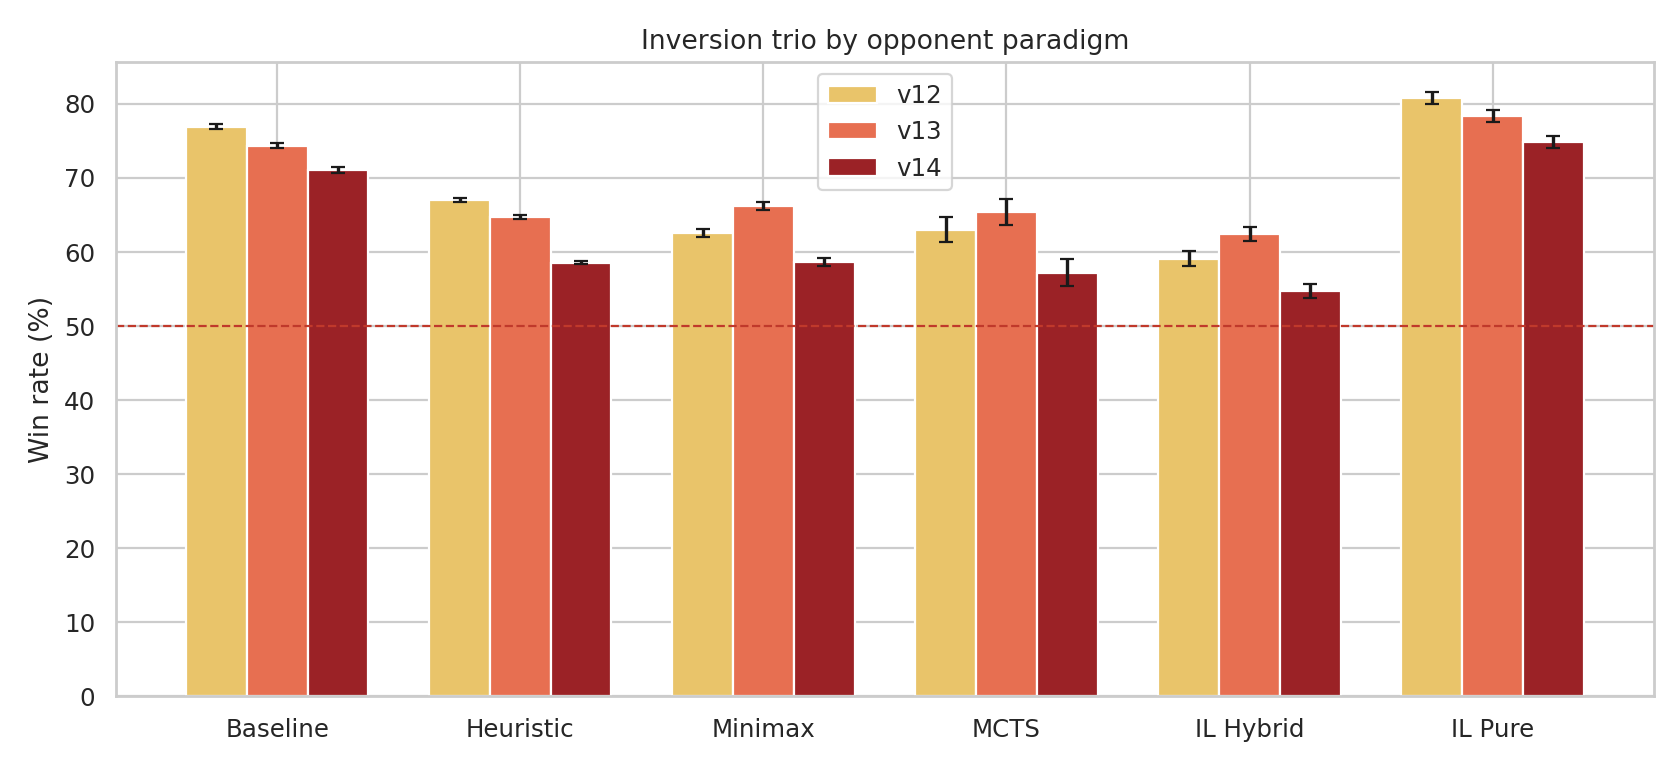
\includegraphics[width=0.95\linewidth]{images/heuristics/heur_wr_by_paradigm.png}
    \caption{Taxa de victòries de la inversió, agregada per paradigma d'oponent. \texttt{v12} és millor contra agents de referència i altres heurístiques; \texttt{v13}, contra minimax, MCTS i imitació híbrida.}
    \label{fig:heur_paradigm}
\end{figure}

En aquest banc de proves, afegir modelatge d'oponents humans redueix el rendiment agent-contra-agent (Figura~\ref{fig:heur_paradigm}). Això indica una possible especialització de domini i justifica mantenir separades la matriu local i l'avaluació pública.

La mostra pública de \texttt{v14} (Secció~\ref{sec:res_ladder}) no permet reordenar \texttt{v12} i \texttt{v14}; de la mateixa manera, la matriu local no permet afirmar quin dels dos obtindria més victòries contra persones.

% ============================================================
\FloatBarrier
\section{Minimax d'un torn}
\label{sec:res_mm}

La pregunta de disseny ---si un maximin d'un torn corregeix \texttt{v14}--- és la de la Secció~\ref{sec:disseny_agents}. Aquí es mesura amb quina freqüència s'executa el mòdul i quan la seva acció difereix de la proposta heurística (Taula~\ref{tab:minimax_head}).

\begin{table}[H]
\centering
\caption{Minimax analític d'un torn (253.000 partides per fila). La cerca s'executa en aproximadament el 16--18\% dels torns. La fulla posicional de \texttt{v16} gairebé no modifica la preparació; el prior de \texttt{v17} redueix la discrepància respecte de \texttt{v14} i obté la taxa més alta de la família.}
\label{tab:minimax_head}
\small
\begin{tabular}{lrrr}
\toprule
 & \textbf{\texttt{v15} HP} & \textbf{\texttt{v16} bonuses} & \textbf{\texttt{v17} prior $+0{,}15$} \\
\midrule
TV global (\%) & 53,80 & 54,30 & \textbf{57,89} \\
IC 95\% (pp) & $\pm 0{,}19$ & $\pm 0{,}19$ & $\pm 0{,}19$ \\
Cerca (\% torns) & 17,6 & 17,6 & 16,3 \\
Discrepància amb \texttt{v14} (\%) & 66,5 & 67,3 & \textbf{36,6} \\
Preparació / partida & 0,21 & 0,21 & 0,21 \\
Perills / partida & 0,05 & 0,04 & 0,04 \\
Tera / partida & 0,40 & 0,39 & 0,38 \\
Pokémon restants & 1,28 & 1,29 & 1,39 \\
\bottomrule
\end{tabular}
\end{table}


\subsection{Freqüència d'intervenció}

Es registren aproximadament 14 comprovacions de debilitament i 4,5 decisions maximin per partida, tal com resumeix l'empremta tàctica de la Figura~\ref{fig:minimax_fp}. La matriu de cerca s'utilitza en el \textbf{16--18\% dels torns}; la resta es resol principalment amb les regles prioritàries heretades.

\begin{quote}
Un agent \texttt{v14} que prioritza debilitaments garantits i aplica una anàlisi maximin d'un torn a les decisions restants.
\end{quote}

Aquest patró és comparable al de \texttt{v21}, que consulta XGBoost en aproximadament el 15\% dels torns, i al de les variants MCTS. Les partides perdudes presenten una discrepància mitjana superior (taxa de \texttt{search\_diff} per torn, detallada a la Figura~\ref{fig:minimax_override}); és una associació, no una prova causal.

\begin{figure}[htbp]
    \centering
    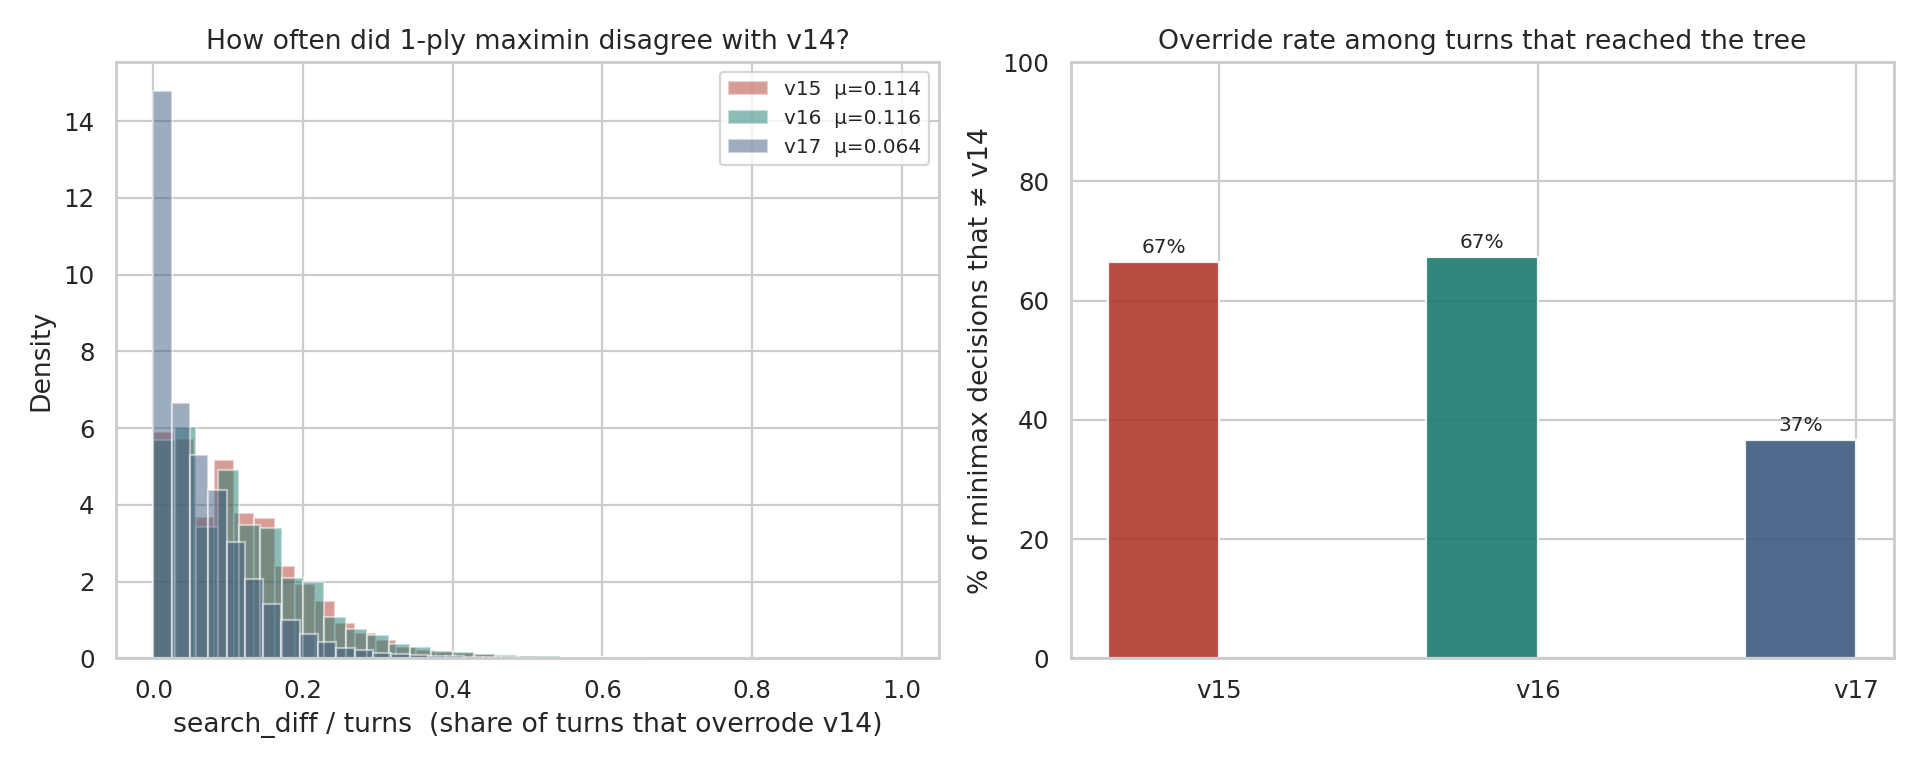
\includegraphics[width=0.92\linewidth]{images/minimax/minimax_override.png}
    \caption{Taxa de discrepància respecte de \texttt{v14} en els torns en què s'executa el maximin. Les barres arrodoneixen a l'enter (67\% / 67\% / 37\%); els valors de la Taula~\ref{tab:minimax_head} són $66{,}5$, $67{,}3$ i $36{,}6$.}
    \label{fig:minimax_override}
\end{figure}

\subsection{\texttt{v16} i l'avaluació de la fulla}

\texttt{v16} incorpora bonificacions per moviments de preparació i perills d'entrada. La taxa global només augmenta 0,50~pp i els enfrontaments directes queden prop del 50\%. Les freqüències de preparació (0,213 i 0,207 per partida) i de perills d'entrada (0,044 i 0,049) pràcticament no canvien. Amb aquesta funció de fulla, el terme de dany rival continua dominant les bonificacions de llarg termini.

La discrepància es manté al voltant del 67\%. Per tant, enriquir la fulla en aquesta magnitud no modifica substancialment la política.

Aquest resultat és coherent amb una limitació d'horitzó: afegir una bonificació estàtica no equival a simular les conseqüències futures d'un moviment de preparació.

\subsection{\texttt{v17}: prior heurístic}

\texttt{v17} afegeix 0,15 al valor de l'acció proposada per \texttt{v14}. La discrepància baixa del $67{,}3\%$ al $36{,}6\%$ i la taxa global augmenta 4,09~pp respecte de \texttt{v15} (diferència altament significativa sobre les 253.000 partides agregades, $z \approx 29{,}3$, $p < 10^{-50}$). En els enfrontaments directes obté $54{,}71\%$ i $54{,}30\%$ contra \texttt{v15} i \texttt{v16} ($n=10.000$; tests de proporció contra paritat $z = 9{,}42$ i $z = 8{,}60$, respectivament, $p < 10^{-17}$ en ambdós casos). El resultat mostra que conservar un prior heurístic és més efectiu, en aquesta implementació, que substituir-lo per la matriu d'un torn.

Contra els comparadors principals, amb $n=10.000$ tret de les cel·les MCTS:

\begin{table}[htbp]
\centering
\small
\caption{Comparativa de les variants Minimax (\texttt{v15}, \texttt{v16}, \texttt{v17}) davant dels principals oponents (taxa de victòries en \%).}
\label{tab:minimax_comparators}
\begin{tabular}{lrrr}
\toprule
Oponent & \texttt{v15} & \texttt{v16} & \texttt{v17} \\
\midrule
\texttt{v12} & 36,04 & 35,92 & \textbf{40,94} \\
\texttt{v13} & 32,82 & 33,50 & 35,10 \\
\texttt{v14} (professor) & 39,43 & 39,56 & \textbf{43,61} \\
Abyssal & 41,72 & 41,86 & \textbf{46,79} \\
\texttt{v20} ($n=1$k) & 39,7 & 44,6 & \textbf{50,4} \\
\texttt{v21} & 43,65 & 44,75 & 47,50 \\
\texttt{v22} & 69,67 & 70,22 & 71,27 \\
\bottomrule
\end{tabular}
\end{table}

\texttt{v17} obté \textbf{43,61\%} contra \texttt{v14}, \textbf{40,94\%} contra \texttt{v12} i 46,79\% contra Abyssal (Taula~\ref{tab:minimax_comparators}). Contra \texttt{v20} obté 50,4\% amb $n=1.000$, un resultat compatible amb rendiments similars en aquell enfrontament.

Cap variant de minimax supera \texttt{v14} o \texttt{v12}. La variant amb millor resultat és precisament la que limita la desviació respecte de l'heurística de partida.

\subsection{Canvis, durada i supervivència}

Pel que fa a la durada dels combats i l'estat final de l'equip, les tres variants de minimax presenten una durada pràcticament coincident, situada al voltant dels 19 torns de mitjana. La millora de \texttt{v17} no prové, per tant, d'allargar sistemàticament les batalles: el seu avantatge rau en una major conservació de recursos, ja que conserva de mitjana 1,39 membres de l'equip al final de la partida, enfront dels 1,28--1,29 membres de \texttt{v15} i \texttt{v16}. Aquesta diferència augmenta significativament la proporció de partides guanyades amb dos o tres membres restants, un patró coherent amb una reducció de decisions maximin agressives que exposaven innecessàriament el Pokémon actiu.

D'altra banda, en la distribució de canvis, \texttt{v17} presenta una mediana superior de canvis voluntaris i de canvis decidits pel mòdul de cerca respecte de \texttt{v15} i \texttt{v16}, tot i discrepar menys de la política base de \texttt{v14}. Aquesta combinació de «més canvis decidits per cerca» i «menys discrepància» no és contradictòria: indica que, quan \texttt{v14} ja aconsella canviar de Pokémon, el prior de $+0{,}15$ afegit a \texttt{v17} reforça el maximin per consolidar aquesta mateixa decisió en lloc de forçar un atac de baix valor. El guany no prové d'un increment indiscriminat del volum brut de canvis, sinó de preservar el criteri de canvi heurístic en estats on una matriu de cerca d'un sol torn manca de la profunditat temporal necessària per ponderar l'atrició a llarg termini, un efecte que es tradueix en un increment de victòries davant d'heurístiques i MCTS (Figura~\ref{fig:minimax_paradigm}).

\begin{figure}[htbp]
    \centering
    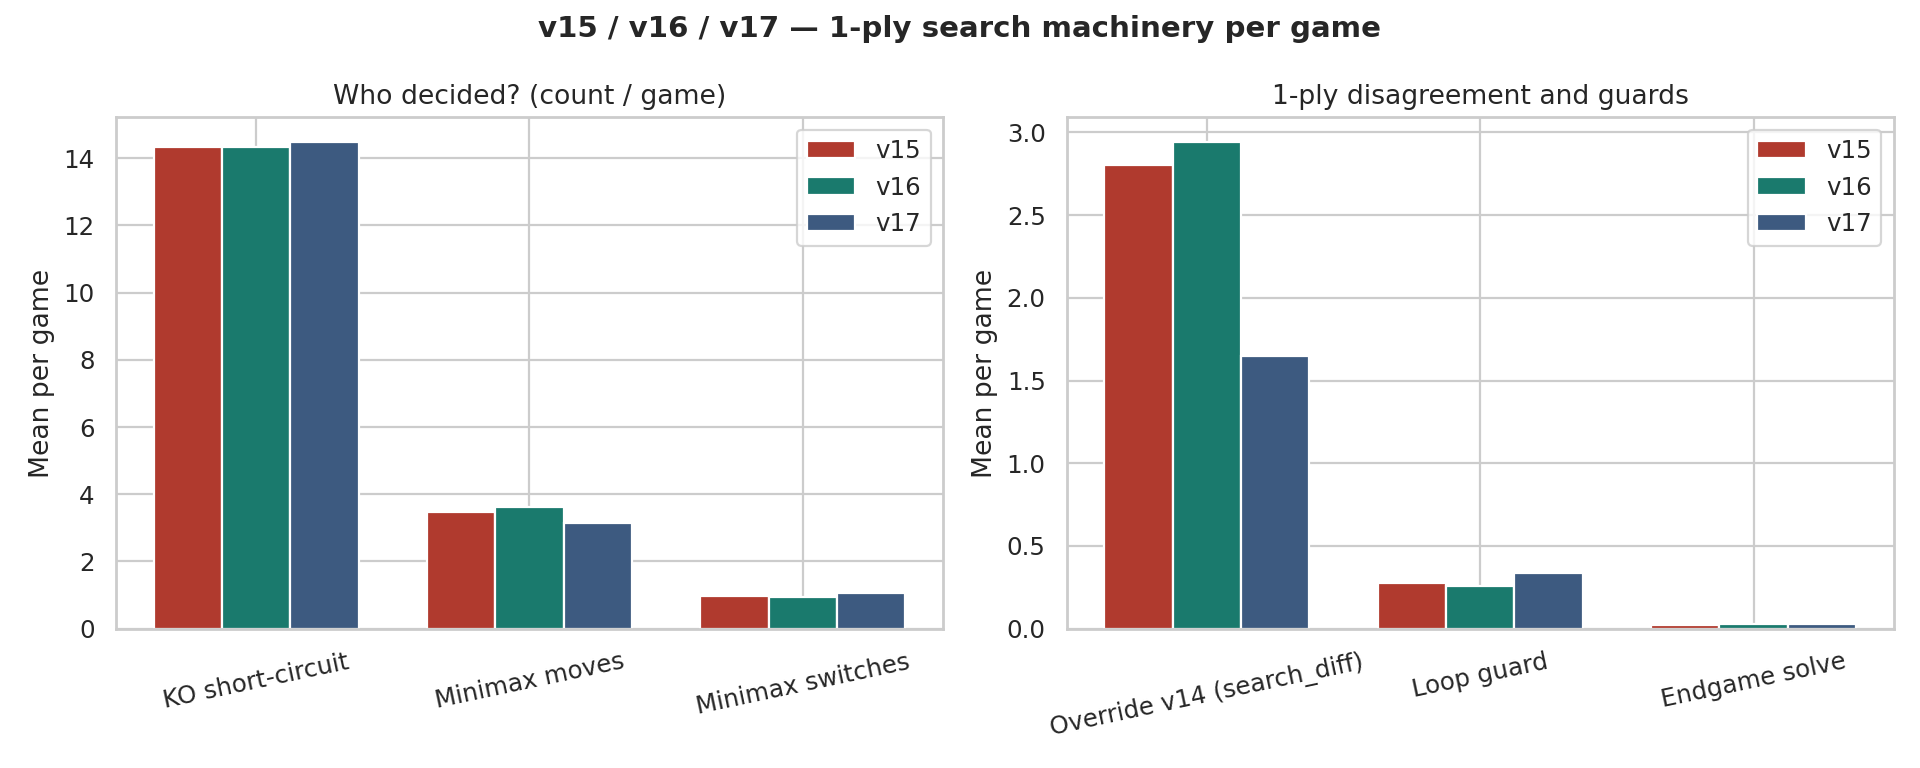
\includegraphics[width=0.92\linewidth]{images/minimax/minimax_fingerprint_bars.png}
    \caption{Empremta \texttt{v15}--\texttt{v17}: KO checks $\sim$14, cerca $\sim$16--18\% dels torns, Tera $\sim$0,39 (nivell \texttt{v14}, no \texttt{v12}).}
    \label{fig:minimax_fp}
\end{figure}

\begin{figure}[htbp]
    \centering
    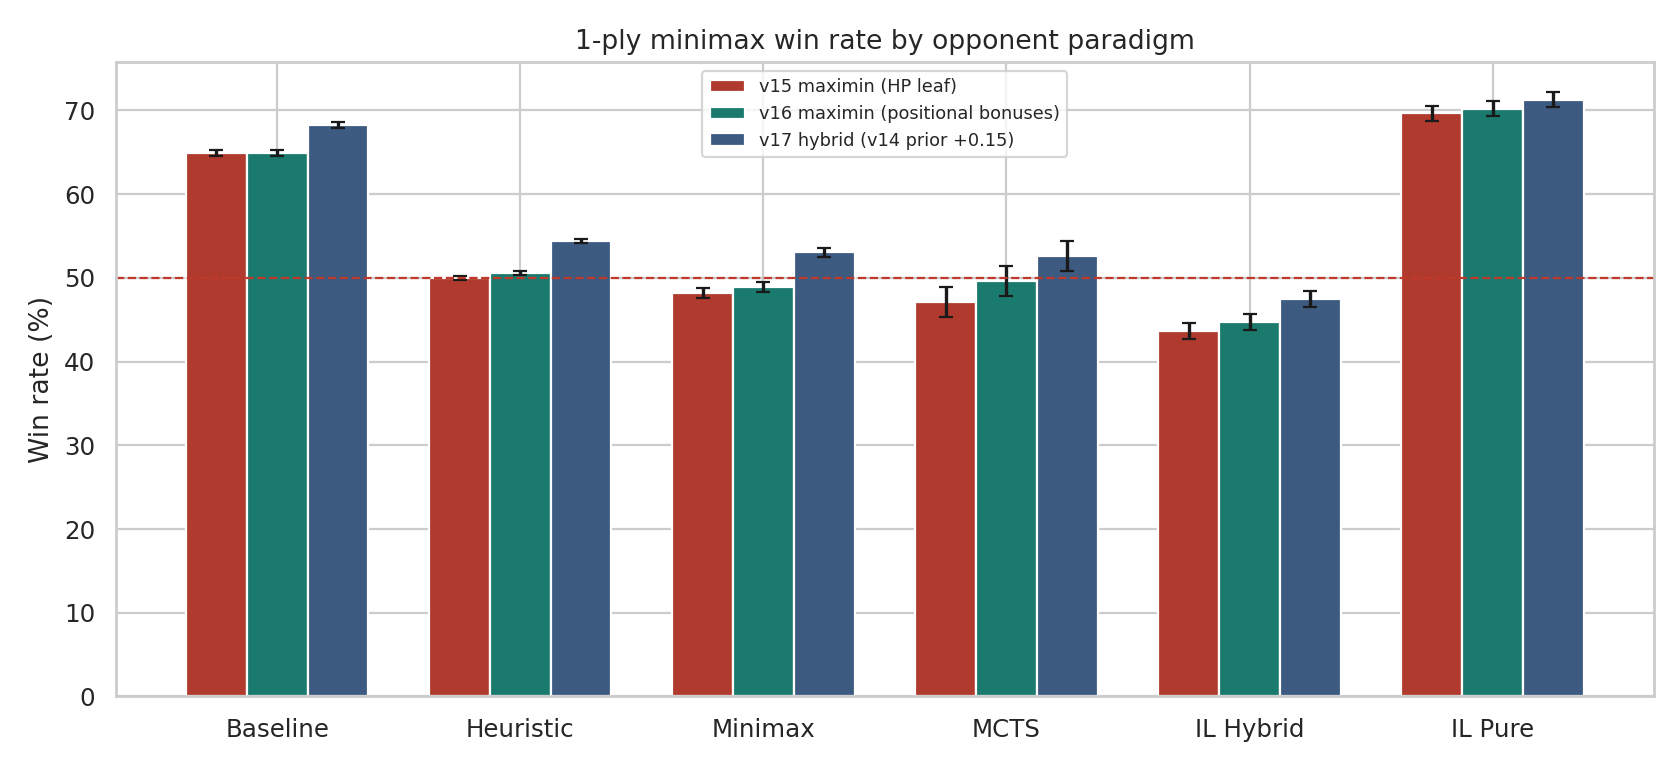
\includegraphics[width=0.92\linewidth]{images/minimax/minimax_wr_by_paradigm.png}
    \caption{Taxa de victòries del minimax per família d'oponent. El prior de \texttt{v17} s'associa amb les millores principals contra heurístiques i MCTS.}
    \label{fig:minimax_paradigm}
\end{figure}

% ============================================================
\FloatBarrier
\section{MCTS ras: UCB a l'arrel i simulacions de cinc torns}
\label{sec:res_mcts}

\textbf{Totes les cel·les d'aquesta secció tenen $n=1.000$} ($\pm 3$~pp, Taula~\ref{tab:ci_n}). La mitjana global de les files MCTS també té una ponderació diferent de la de les files no MCTS. La pregunta de disseny ---si cinc torns simulats superen l'horitzó de \texttt{v14}--- és la de la Secció~\ref{sec:disseny_agents}, amb els registres principals resumits a la Taula~\ref{tab:mcts_head}.

\begin{table}[H]
\centering
\caption{IS-MCTS (100 simulacions $\times$ 5 torns de \texttt{LocalSim}). \textbf{Totes les cel·les $n=1.000$}; 28.000 partides per agent; IC global $\approx\pm 0{,}58$~pp, IC per cel·la $\approx\pm 3{,}1$~pp. Una fulla més rica (\texttt{v19}) no ajuda. PUCT amb prior 0,70 sobre \texttt{v14} (\texttt{v20}) és l'única millora, perquè discrepa \emph{menys}.}
\label{tab:mcts_head}
\small
\begin{tabular}{lrrr}
\toprule
 & \textbf{\texttt{v18} UCB1 HP} & \textbf{\texttt{v19} UCB1 pos.} & \textbf{\texttt{v20} PUCT 0,70} \\
\midrule
WR global (\%) & 54,02 & 53,29 & \textbf{59,66} \\
Cerca (\% torns) & 18,1 & 17,6 & 15,5 \\
Override de \texttt{v14} (\%) & 71,3 & 71,1 & \textbf{18,7} \\
Setup / partida & 0,22 & 0,22 & 0,20 \\
Hazards / partida & 0,05 & 0,05 & 0,04 \\
Tera / partida & 0,41 & 0,39 & 0,39 \\
Mons restants (nosaltres) & 1,21 & 1,22 & 1,40 \\
\bottomrule
\end{tabular}
\end{table}


\texttt{v20} obté una taxa superior a \texttt{v18} en els \textbf{28 enfrontaments} (diferència mitjana de 5,64~pp). \texttt{v18} i \texttt{v19} queden prop del 50\% en l'enfrontament directe, mentre que \texttt{v20} obté aproximadament 56,6\% contra tots dos. En aquest pressupost, enriquir només la funció de fulla de \texttt{v19} no aporta una millora observable.

\subsection{Freqüència d'intervenció}

Es registren aproximadament 14 comprovacions de debilitament i 3--4 decisions MCTS per partida. La cerca intervé en el \textbf{15--18\%} dels torns:

\begin{quote}
Un agent basat en \texttt{v14} que prioritza els debilitaments garantits i aplica 100 simulacions de cinc torns a les decisions restants.
\end{quote}

Quan s'activa una drecera prèvia, les 100 simulacions no s'executen. Per tant, la cerca només pot modificar el subconjunt de decisions que arriba a l'arrel.

\begin{figure}[htbp]
    \centering
    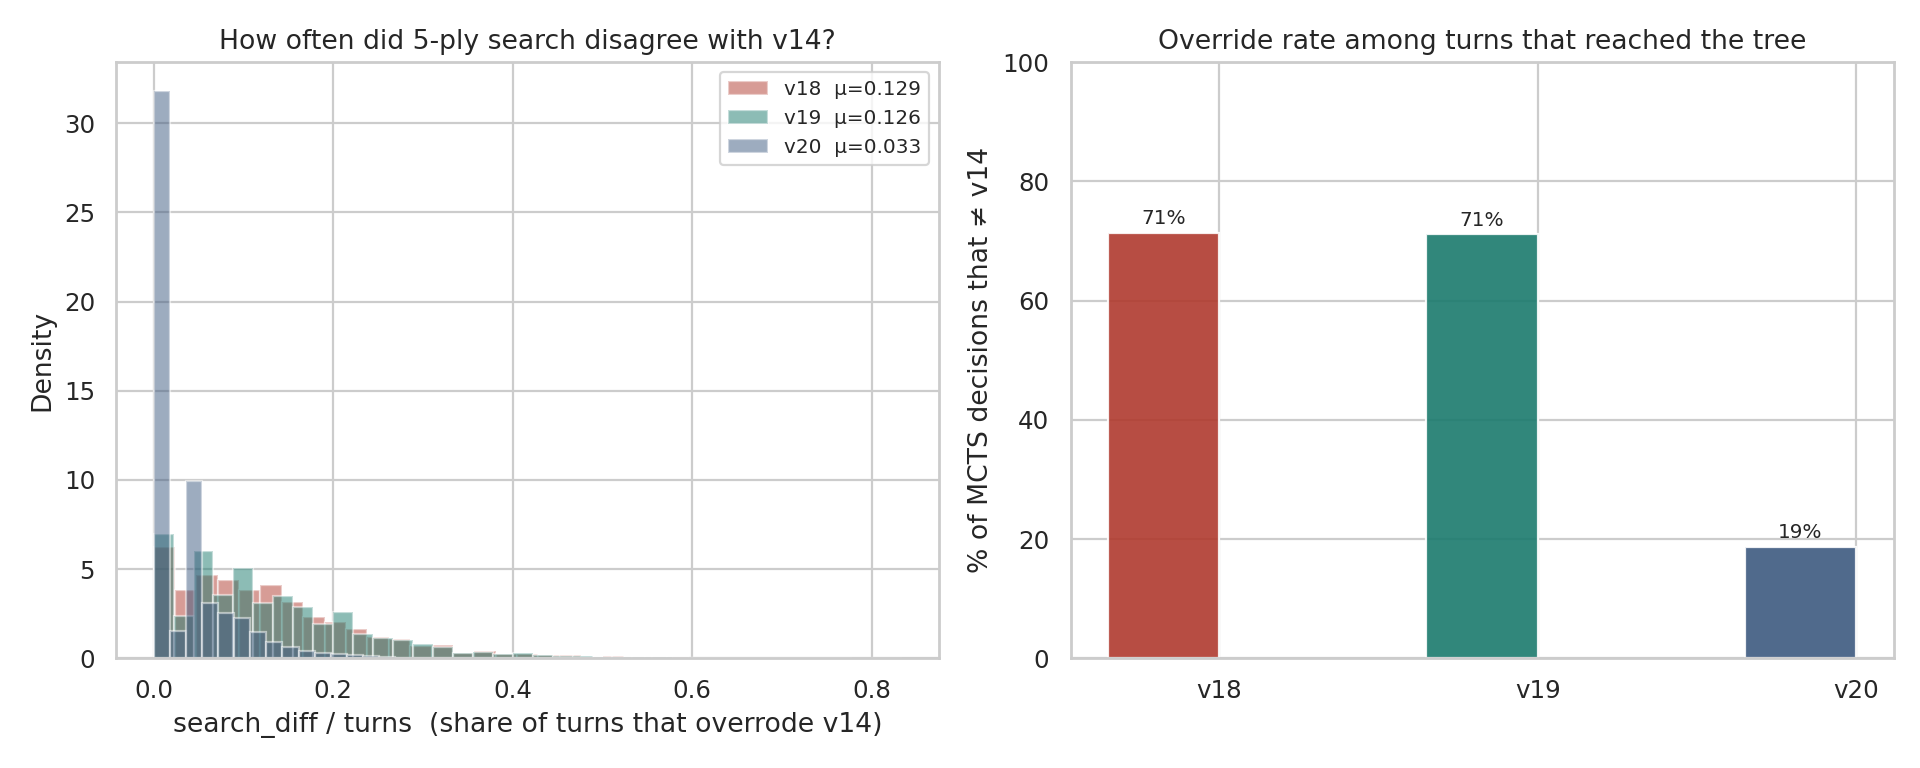
\includegraphics[width=0.92\linewidth]{images/mcts/mcts_override.png}
    \caption{Taxa de discrepància respecte de \texttt{v14} entre les decisions de cerca. Les barres arrodoneixen a l'enter (71\% / 71\% / 19\%); els valors de la Taula~\ref{tab:mcts_head} són $71{,}3$, $71{,}1$ i $18{,}7$.}
    \label{fig:mcts_override}
\end{figure}

\subsection{Discrepància i resultat}

\texttt{search\_diff} indica que la simulació ha canviat l'acció proposada per \texttt{v14}. Entre els torns en què s'executa:

\begin{itemize}
    \item \texttt{v18}/\texttt{v19} discrepen de \texttt{v14} en el \textbf{71,3\%} i el \textbf{71,1\%} de les decisions de cerca, respectivament, mentre que el prior PUCT de \texttt{v20} redueix aquesta taxa al 18,7\% (Figura~\ref{fig:mcts_override}).
    \item Les partides perdudes presenten una discrepància superior. Aquest patró pot reflectir decisions pitjors, estats més difícils o ambdues coses.
    \item Les simulacions de cinc torns i la funció de fulla basada en HP poden afavorir el dany immediat davant d'efectes diferits.
\end{itemize}

\texttt{v19} incorpora una fulla posicional, però manté una discrepància del 71,1\% i una taxa global 0,7~pp inferior a \texttt{v18}. Les dades no mostren que aquest canvi de fulla resolgui les limitacions del pressupost, de la política de simulació o de la informació oculta.

\subsection{PUCT i el prior heurístic}

Amb un prior de 0,70 sobre \texttt{v14}, la discrepància baixa al \textbf{18,7\%}. \texttt{v20} obté una taxa global descriptiva de \textbf{59,66\%} i conserva 1,40 Pokémon de mitjana al final.

Les diferències de \texttt{v20} respecte de \texttt{v18} són especialment grans contra \texttt{v17} (+11,1~pp), \texttt{v13} (+10,5), \texttt{v15} (+9,8) i \texttt{v12} (+8,7). Contra \texttt{random}, la diferència és de 0,3~pp i queda molt per sota de la precisió de la cel·la.

Amb aquest pressupost, la millor variant MCTS és la que utilitza les simulacions per ajustar un prior heurístic, no la que substitueix l'heurística amb UCB1 sense guia.

\subsection{Indicadors d'efectes diferits}

A la Taula~\ref{tab:deferred_effects} es resumeixen les taxes d'activació de mecàniques diferides per partida segons paradigma.

\begin{table}[htbp]
\centering
\small
\caption{Freqüències mitjanes d'activació de mecàniques diferides (\emph{setup}, \emph{hazards} i Teracristal·lització per partida) segons paradigma.}
\label{tab:deferred_effects}
\begin{tabular}{lrrr}
\toprule
 & Setup/partida & Hazards/partida & Tera/partida \\
\midrule
\texttt{v12} (comparador) & $\sim$1,75 & $\sim$0,18 & $\sim$0,96 \\
\texttt{v14} (professor) & $\sim$0,21 & $\sim$0,03 & $\sim$0,34 \\
Minimax d'un torn \texttt{v15}--\texttt{v17} & 0,21 & 0,04--0,05 & 0,38--0,40 \\
MCTS de cinc torns \texttt{v18}--\texttt{v20} & 0,20--0,22 & 0,04--0,05 & 0,39--0,41 \\
\bottomrule
\end{tabular}
\end{table}

Les freqüències de preparació i perills d'entrada es mantenen a nivells semblants als de \texttt{v14}, no als de \texttt{v12}. Les simulacions de cinc torns no recuperen, amb aquesta política, el comportament diferit observat a l'heurística amb millor taxa.

\texttt{v20} presenta més \texttt{search\_switches} (aproximadament 36\% de les decisions de cerca, davant del 16\% a \texttt{v18}) i menys discrepància total. Això indica que PUCT reforça sovint els canvis ja proposats per \texttt{v14}.

\subsection{Comparació amb els agents de referència}

\begin{table}[htbp]
\centering
\small
\caption{Rendiment de les variants MCTS (\texttt{v18}, \texttt{v19}, \texttt{v20}) davant dels oponents de referència (taxa de victòries en \%).}
\label{tab:mcts_comparators}
\begin{tabular}{lrrr}
\toprule
Oponent & \texttt{v18} & \texttt{v19} & \texttt{v20} \\
\midrule
\texttt{v12} & 34,0 & 33,1 & \textbf{42,7} \\
\texttt{v13} & 28,6 & 34,1 & 39,1 \\
\texttt{v14} & 40,0 & 41,7 & \textbf{47,0} \\
Abyssal & 42,2 & 38,7 & \textbf{49,0} \\
\texttt{v15} & 49,3 & 51,6 & \textbf{59,1} \\
\texttt{v17} & 44,7 & 45,3 & 55,8 \\
\texttt{v21} & 44,1 & 46,5 & 49,6 \\
\texttt{v22} & 71,1 & 66,9 & 73,0 \\
\bottomrule
\end{tabular}
\end{table}

\texttt{v20} obté \textbf{47,0\%} contra \texttt{v14}, \textbf{42,7\%} contra \texttt{v12} i \textbf{49,0\%} contra Abyssal (Taula~\ref{tab:mcts_comparators}). Amb $n=1.000$, el primer i el tercer resultat són compatibles amb la paritat del 50\% ($z = -1{,}90$, $p = 0{,}057$ i $z = -0{,}63$, $p = 0{,}53$, no significatius al nivell $\alpha=0{,}05$). En canvi, el desavantatge davant \texttt{v12} és significatiu ($z = -4{,}62$, $p < 10^{-5}$), i els avantatges davant \texttt{v15} (59,1\%, $z = 5{,}76$, $p < 10^{-8}$) i \texttt{v22} (73,0\%, $z = 14{,}55$, $p < 10^{-15}$) són estadísticament inequívocs.

Per blocs (Figura~\ref{fig:mcts_paradigm}), \texttt{v20} obté 69,9\% contra agents de referència, 56,7\% contra heurístiques i 57,4\% contra minimax. \texttt{v18}/\texttt{v19} se situen prop del 50\% contra heurístiques i per sota del 50\% contra minimax.

L'MCTS ras amb 100 simulacions de cinc torns no supera \texttt{v12} ni aporta evidència de superar \texttt{v14}. Dins de la família, el prior heurístic de \texttt{v20} és el canvi associat amb la millora principal.

\subsection{Canvis, durada i supervivència}

En l'anàlisi de la durada dels combats i la supervivència de l'equip, \texttt{v20} conclou les batalles lleugerament abans (18,33 torns de mitjana) i conserva 1,40 membres de l'equip al final de la partida, davant dels 1,21--1,22 membres que aconsegueixen preservar les variants d'UCB1 pur (\texttt{v18} i \texttt{v19}). El patró de \texttt{v20} no és, per tant, el d'una política excessivament defensiva que es limita a prolongar els enfrontaments: tanca les partides amb més rapidesa i preservant més recursos. Una explicació plausible és que el guiatge heurístic del prior desaconsella branques de simulació miops que opten per dany immediat a costa d'un enfrontament clarament desfavorable al torn següent.

Pel que fa a la dinàmica de canvis, l'algorisme PUCT augmenta de manera substancial la fracció de decisions de cerca que acaben en canvi i n'eixampla la distribució de canvis voluntaris. Mentre que \texttt{v18} gairebé mai escull un canvi des de l'arrel en la mediana de partides, a \texttt{v20} aproximadament un terç de les decisions preses pel mòdul de cerca corresponen a canvis de Pokémon. Com que al mateix temps la taxa de discrepància \texttt{search\_diff} cau fins al 18,7\%, aquests canvis solen coincidir amb la recomanació del coneixement expert de \texttt{v14}. Aquesta convergència reforça la interpretació que la millora de PUCT rau en consolidar i no degradar la posició tàctica proposada per l'heurística (com reflecteix l'empremta tàctica de la Figura~\ref{fig:mcts_fp}), més que en la descoberta d'estratègies noves en un horitzó de cinc torns.

\begin{figure}[htbp]
    \centering
    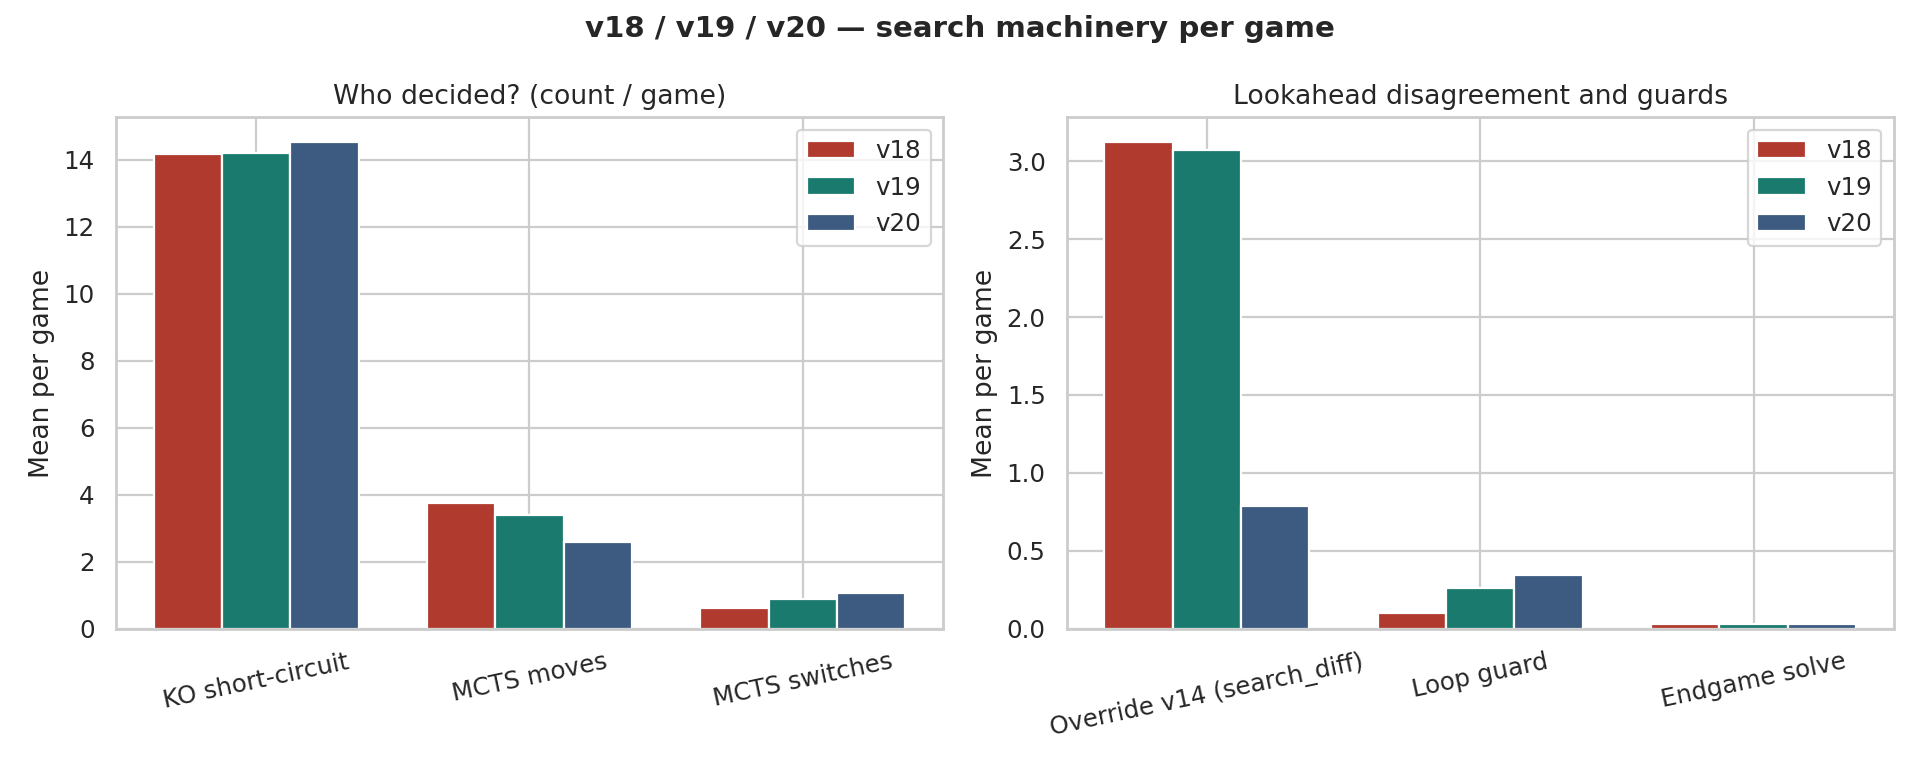
\includegraphics[width=0.92\linewidth]{images/mcts/mcts_fingerprint_bars.png}
    \caption{Empremta MCTS. Cerca 15--18\% dels torns (\texttt{v20}: $15{,}5\%$); KO $\sim$14/partida. \texttt{v20} busca menys i acaba amb més HP. $n=1.000$ per oponent.}
    \label{fig:mcts_fp}
\end{figure}

\begin{figure}[htbp]
    \centering
    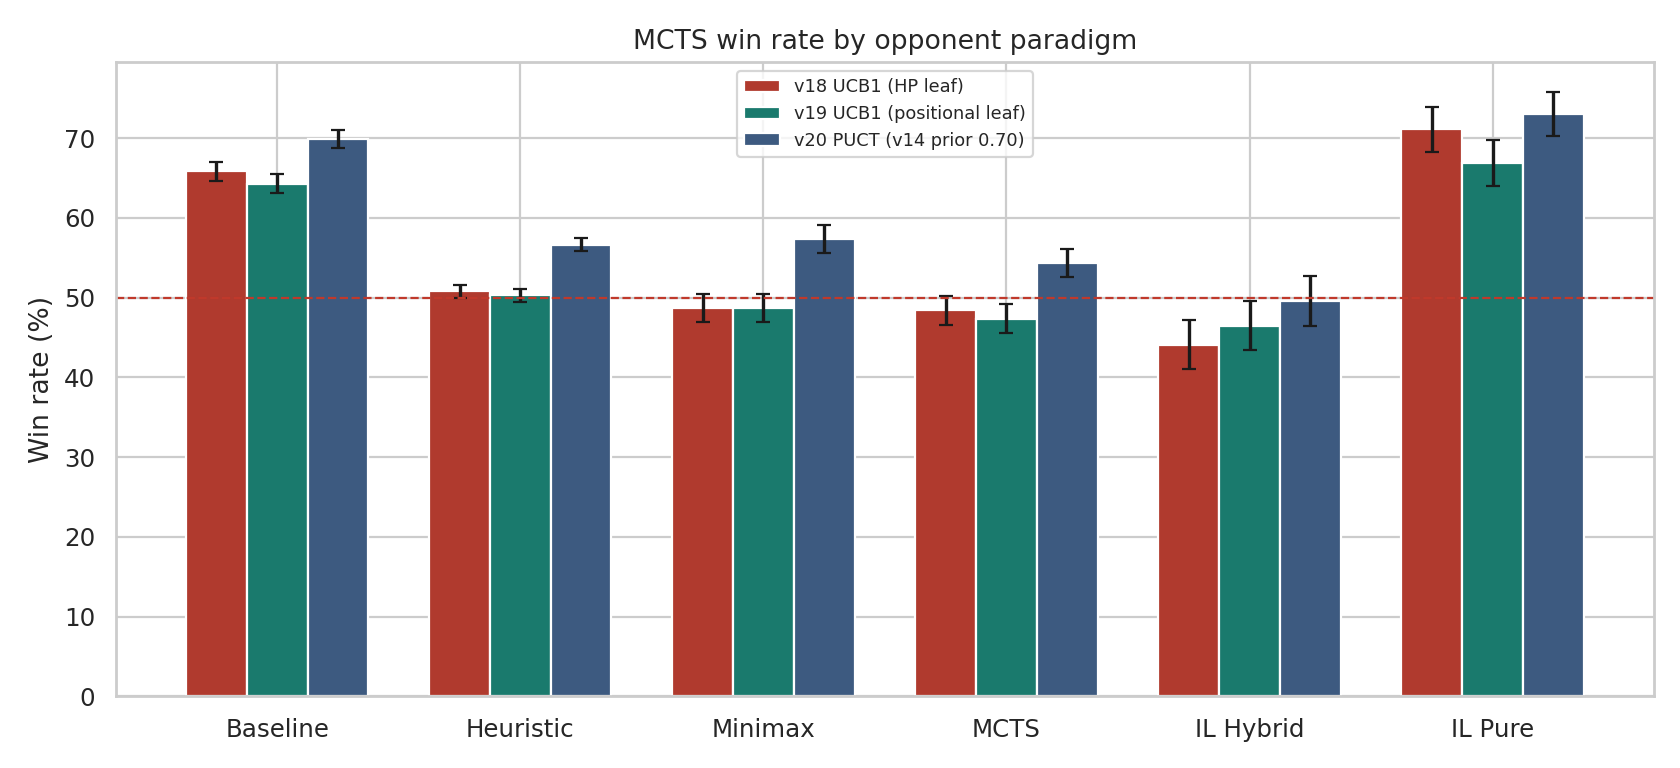
\includegraphics[width=0.92\linewidth]{images/mcts/mcts_wr_by_paradigm.png}
    \caption{Taxa de victòries d'MCTS per paradigma d'oponent ($n=1.000$ a cada cel·la). PUCT millora principalment contra heurístiques i minimax.}
    \label{fig:mcts_paradigm}
\end{figure}

% ============================================================
\FloatBarrier
\section{Aprenentatge per imitació: dues formes d'execució}
\label{sec:res_il}

Les dues variants comparteixen el classificador XGBoost i el llindar $\tau=0{,}5525$ del Capítol~\ref{chap:implementacio}, però difereixen en la selecció de l'acció concreta (Taula~\ref{tab:il_head}).

\begin{table}[H]
\centering
\caption{Imitació amb el mateix classificador XGBoost ($\tau=0{,}5525$) i dues formes d'execució (253.000 partides per fila). \texttt{v21} consulta el model en el 15\% dels torns; \texttt{v22}, en el 80\%, sense proteccions de debilitament, i activa la protecció de bucle en el 97\% de les partides.}
\label{tab:il_head}
\small
\begin{tabular}{lrr}
\toprule
 & \textbf{\texttt{v21} híbrid} & \textbf{\texttt{v22} atributs} \\
\midrule
TV global (\%) & \textbf{58,71} $\pm 0{,}19$ & 33,49 $\pm 0{,}18$ \\
Torns mitjans & 18,20 & 20,07 \\
Pokémon restants & 1,33 & 0,70 \\
Canvis voluntaris / partida & 1,98 & 3,72 \\
XGBoost (\% torns) & 15,2 & 79,9 \\
Entre decisions XGB, \% canvis & 35,5 & 15,2 \\
Mitjana $p(\mathrm{canvi})$ & 0,080 & 0,351 \\
Proteccions de KO / partida & 13,85 & \textbf{0} \\
Resolucions de final / partida & 0,032 & \textbf{0} \\
Proteccions de bucle / partida (\% partides) & 0,38 (33\%) & 1,92 (\textbf{97\%}) \\
\bottomrule
\end{tabular}
\end{table}


\texttt{v21} obté una taxa superior a \texttt{v22} en els \textbf{28 enfrontaments} (Figura~\ref{fig:il_scatter}), amb una diferència mitjana de 25,2~pp. En el cara a cara, les dues orientacions són 71,74\% i 29,07\%; l'autojoc queda prop del 50\%. A \texttt{v22}, els comptadors \texttt{ko\_guards}, \texttt{endgame\_solves}, \texttt{ko\_checks} i \texttt{search\_*} són zero, fet que confirma que no executa les dreceres de \texttt{v14}, com s'observa a l'empremta tàctica comparativa de la Figura~\ref{fig:il_fp}.

\begin{figure}[htbp]
    \centering
    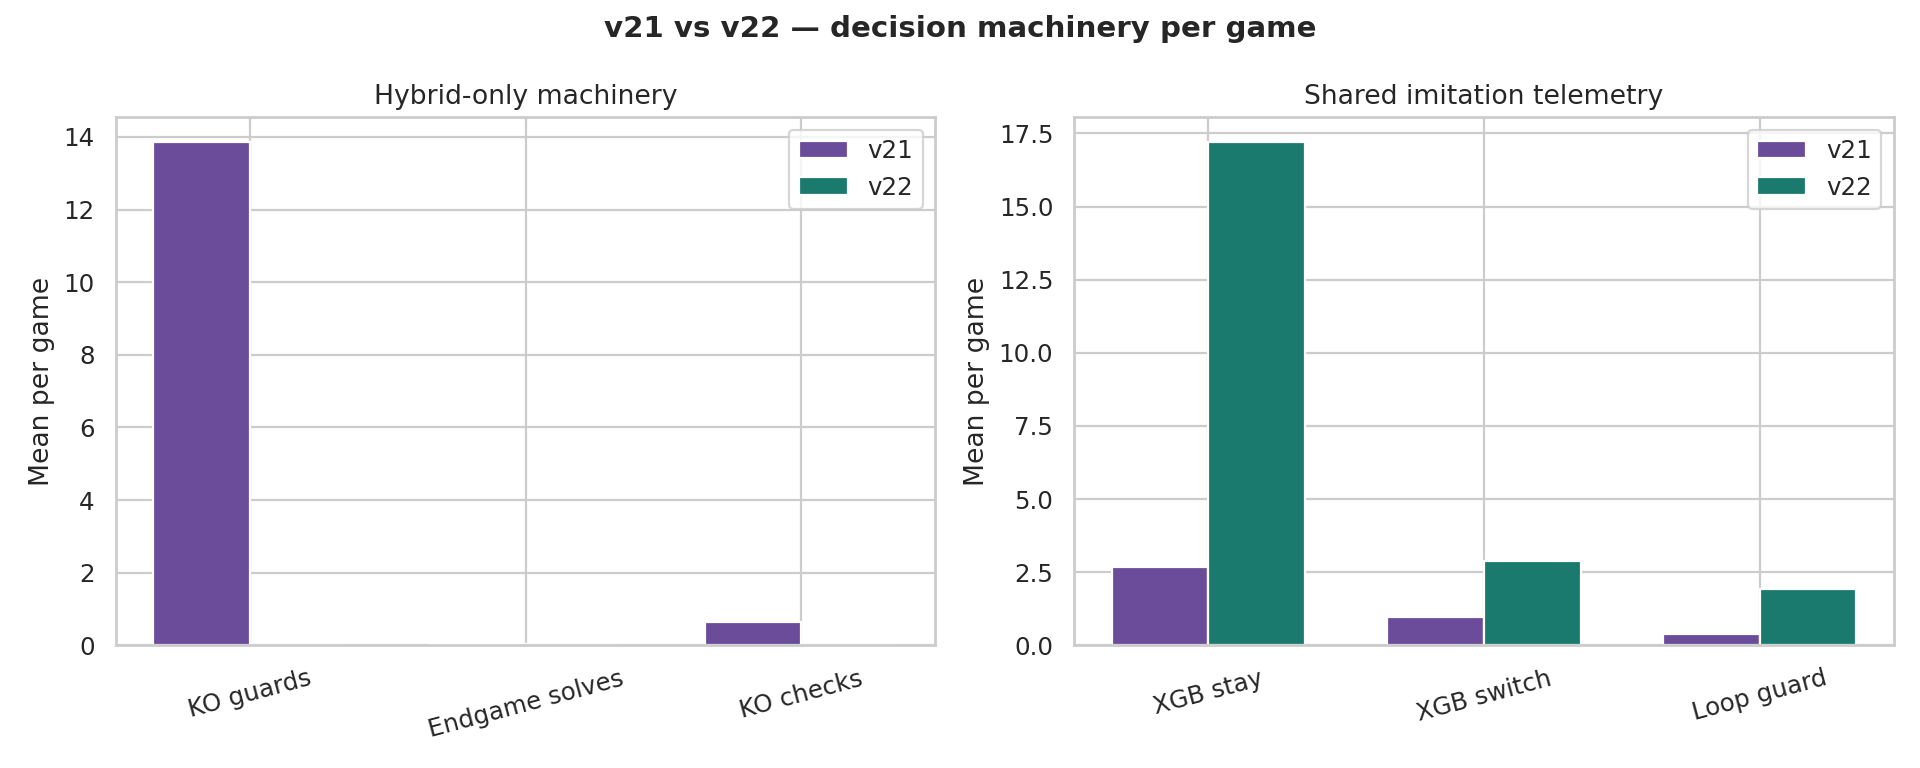
\includegraphics[width=0.92\linewidth]{images/il/il_fingerprint_bars.png}
    \caption{Empremta dels agents d'imitació. \texttt{v21} registra aproximadament 14 proteccions de debilitament per partida; \texttt{v22} no. El panell dret mostra que \texttt{v22} consulta XGBoost moltes més vegades i activa més sovint la protecció de bucle.}
    \label{fig:il_fp}
\end{figure}

\subsection{Rendiment dins de la matriu}

\texttt{v21} obté una taxa global descriptiva de 58,71\%, propera a \texttt{v9}/\texttt{v11}. \texttt{v22} obté 33,49\%, per sota de \texttt{v1} (44,25\%). En l'enfrontament directe, \texttt{v1} guanya el 65,72\% de les partides contra \texttt{v22}.

Enfrontaments de referència ($n=10.000$, tret de \texttt{v20}, Taula~\ref{tab:il_comparators}):

\begin{table}[htbp]
\centering
\small
\caption{Comparació de rendiment dels models d'imitació jeràrquica (\texttt{v21}, \texttt{v22}) enfront de la cerca i referències (taxa de victòries en \%).}
\label{tab:il_comparators}
\begin{tabular}{lrrrrr}
\toprule
 & contra \texttt{v12} & contra \texttt{v13} & contra \texttt{v14} & contra Abyssal & contra SimpleH \\
\midrule
\texttt{v21} & 41,28 & 38,39 & 45,43 & 46,98 & 47,76 \\
\texttt{v17} & 40,94 & 35,10 & 43,61 & 46,79 & 46,75 \\
\texttt{v20} ($n=1$k) & 42,7 & 39,1 & 47,0 & 49,0 & 49,2 \\
\texttt{v22} & 19,80 & 22,03 & 25,81 & 22,90 & 21,73 \\
\bottomrule
\end{tabular}
\end{table}

\texttt{v14} obté 54,74\% contra \texttt{v21}, i l'orientació recíproca és 45,43\%. Per tant, afegir el model de decisió atacar/canviar no millora \texttt{v14} en aquest enfrontament. Les taxes contra Abyssal són 46,98\% i 51,36\%, respectivament.

\subsection{Pes efectiu del model a \texttt{v21}}

Només el \textbf{15\%} dels torns arriben a XGBoost (Figura~\ref{fig:il_fire}); les regles prèvies de \texttt{v14} resolen la resta. En els torns consultats, la probabilitat mitjana de canvi és 0,08, molt inferior a $\tau=0{,}5525$. En conseqüència, el model sol indicar que l'agent es mantingui al camp i \texttt{v14} selecciona el moviment.

Descripció honesta:

\begin{quote}
Un agent \texttt{v14} que, en una fracció minoritària dels torns, consulta un model d'imitació per decidir si convé canviar i delega l'execució concreta a la mateixa heurística.
\end{quote}

La capa d'imitació funciona, doncs, com un \textbf{prior sobre el moment de canviar}, no com un motor tàctic complet. Aquesta descripció és important per no atribuir tot el rendiment de \texttt{v21} al model supervisat.

La comparació mostra que la decisió d'alt nivell es pot integrar de manera útil quan l'acció concreta queda restringida per una política competent. No mostra que el classificador, per si sol, reprodueixi el joc expert.

\begin{figure}[htbp]
    \centering
    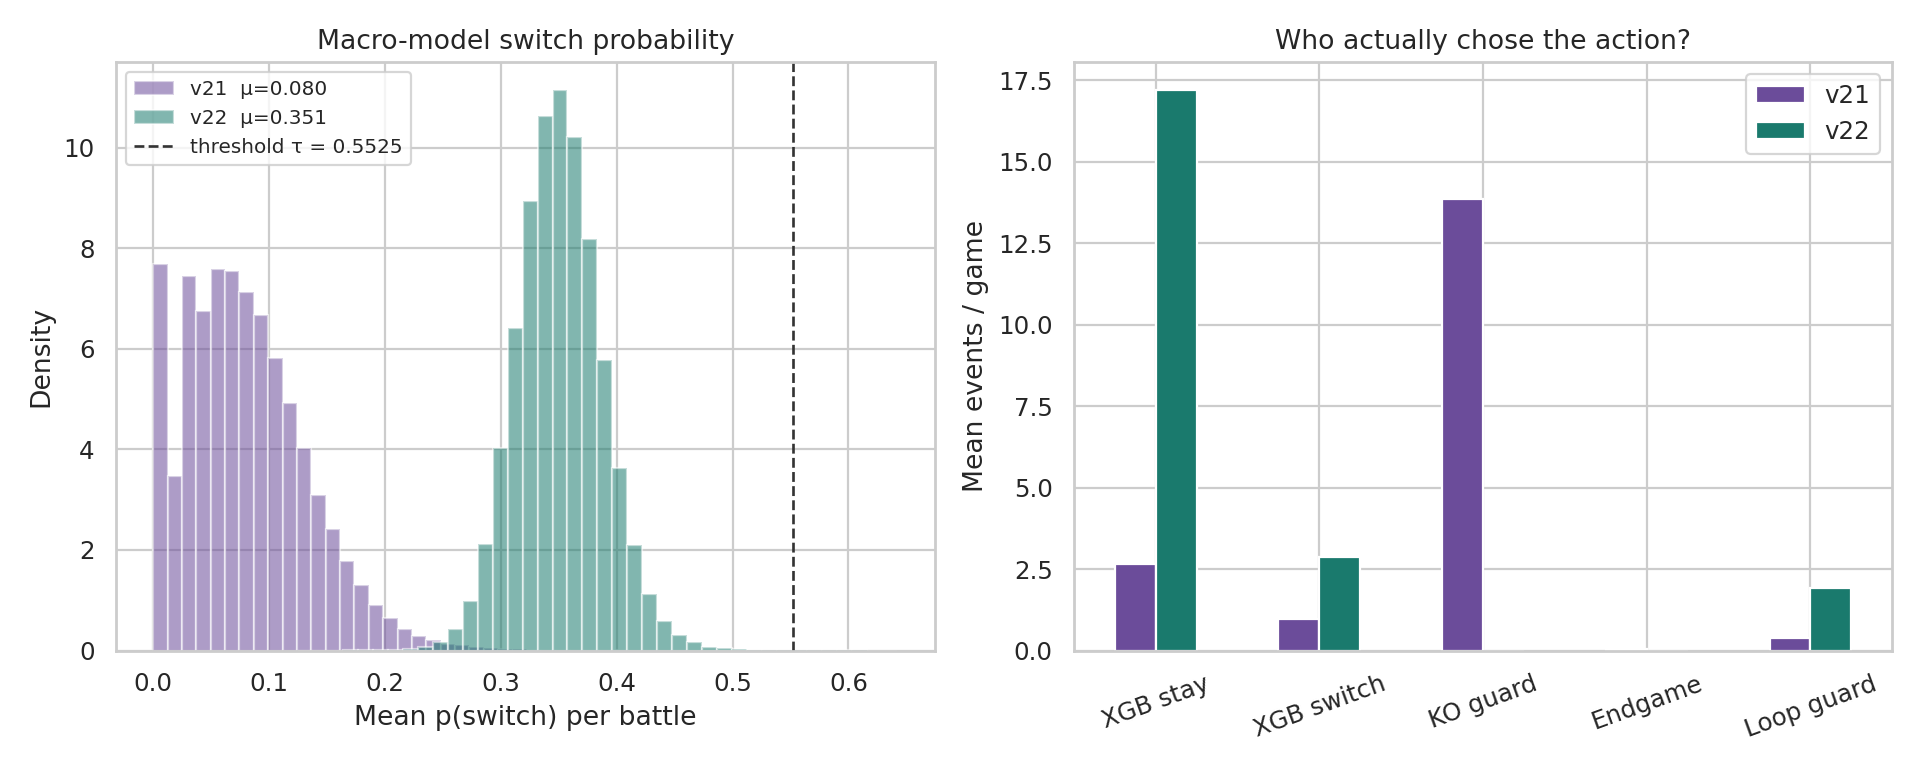
\includegraphics[width=0.92\linewidth]{images/il/il_policy_firing.png}
    \caption{Freqüència d'ús de la política apresa. XGBoost intervé en el 15\% dels torns de \texttt{v21} i en el 80\% dels de \texttt{v22}.}
    \label{fig:il_fire}
\end{figure}

\subsection{Factors que limiten \texttt{v22}}

\begin{enumerate}
    \item \textbf{Semàntica de l'acció.} El primer model només prediu $\{\mathrm{atacar},\mathrm{canviar}\}$ i el segon puntua atributs de candidats sintetitzats. Es perd informació sobre la identitat i el context del moviment.
    \item \textbf{Biaix d'exposició.} Una decisió deficient pot portar la política a estats poc representats a les repeticions. La protecció de bucle s'activa en el \textbf{97\%} de les partides de \texttt{v22}, que també són més llargues i acaben amb menys Pokémon disponibles.
    \item \textbf{Absència de restriccions tàctiques.} \texttt{v21} preserva els debilitaments garantits abans de consultar el model; \texttt{v22} no. La freqüència de Teracristal·lització de \texttt{v22} és alta (gairebé una vegada per partida, enfront d'un ús selectiu i conservador a \texttt{v21} heretat de \texttt{v14}, $\sim 0{,}34$ per partida), però la freqüència per si sola no informa de la qualitat del moment triat.
\end{enumerate}

En aquesta implementació, el resultat depèn tant de \emph{què} s'imita ---la decisió atacar/canviar--- com de \emph{qui} executa l'acció concreta. Disposar d'1,12 milions de torns no compensa una representació que no modela directament la selecció completa de moviments i canvis.

El contrast entre \texttt{v21} i \texttt{v22} no compara únicament dos models d'imitació: també compara una arquitectura jeràrquica amb una execució basada en atributs. Aquesta confusió de factors impedeix atribuir els 25,2~pp exclusivament a una sola decisió de disseny, però demostra la importància de l'executor.

\subsection{Canvis, durada i supervivència}

Pel que fa a la durada de les partides i l'estat final de l'equip, \texttt{v22} registra partides significativament més llargues (amb una mitjana de 20,07 torns) però conclou amb només 0,70 membres de l'equip disponibles de mitjana, en clar contrast amb els 1,33 membres que aconsegueix preservar \texttt{v21}. Aquesta major durada temporal de \texttt{v22} no és en cap cas indicativa de control tàctic o domini posicional: en anar acompanyada d'un nombre tan reduït de supervivents i d'una taxa global de victòria molt menor (33,49\%), reflecteix una dinàmica de canvis que retarda el debilitament inevitable sense arribar a estabilitzar mai la posició. Aquest patró concorda plenament amb el biaix d'exposició de l'aprenentatge per imitació: després d'un canvi subòptim o descontextualitzat, el model es veu obligat a prendre decisions successives en estats allunyats de la distribució de les trajectòries humanes d'entrenament, repercutint en una pèrdua d'eficàcia transversal en tots els paradigmes rivals (Figura~\ref{fig:il_paradigm}).

Aquesta dinàmica es reflecteix directament en la distribució dels canvis. Mentre que els canvis forçats presenten volums similars entre totes dues variants (en dependre primordialment dels debilitaments soferts), la diferència fonamental rau en els canvis voluntaris i en les consultes a XGBoost: \texttt{v22} executa aproximadament el doble de canvis voluntaris que \texttt{v21} i rep moltes més instruccions de canvi del classificador. La distribució de \texttt{v22} es concentra al voltant de 3 o 4 canvis voluntaris per partida, mentre que \texttt{v21} en realitza habitualment entre 1 i 2. Si es combina aquest patró amb el fet que el mecanisme de protecció contra bucles de canvis s'activa en el 97\% de les partides de \texttt{v22}, l'evidència suggereix que el factor limitant no és la manca de propensió al canvi, sinó l'absència d'un executor capaç de ponderar el destí de la transició i el cost tàctic de revertir-la.

\begin{figure}[htbp]
    \centering
    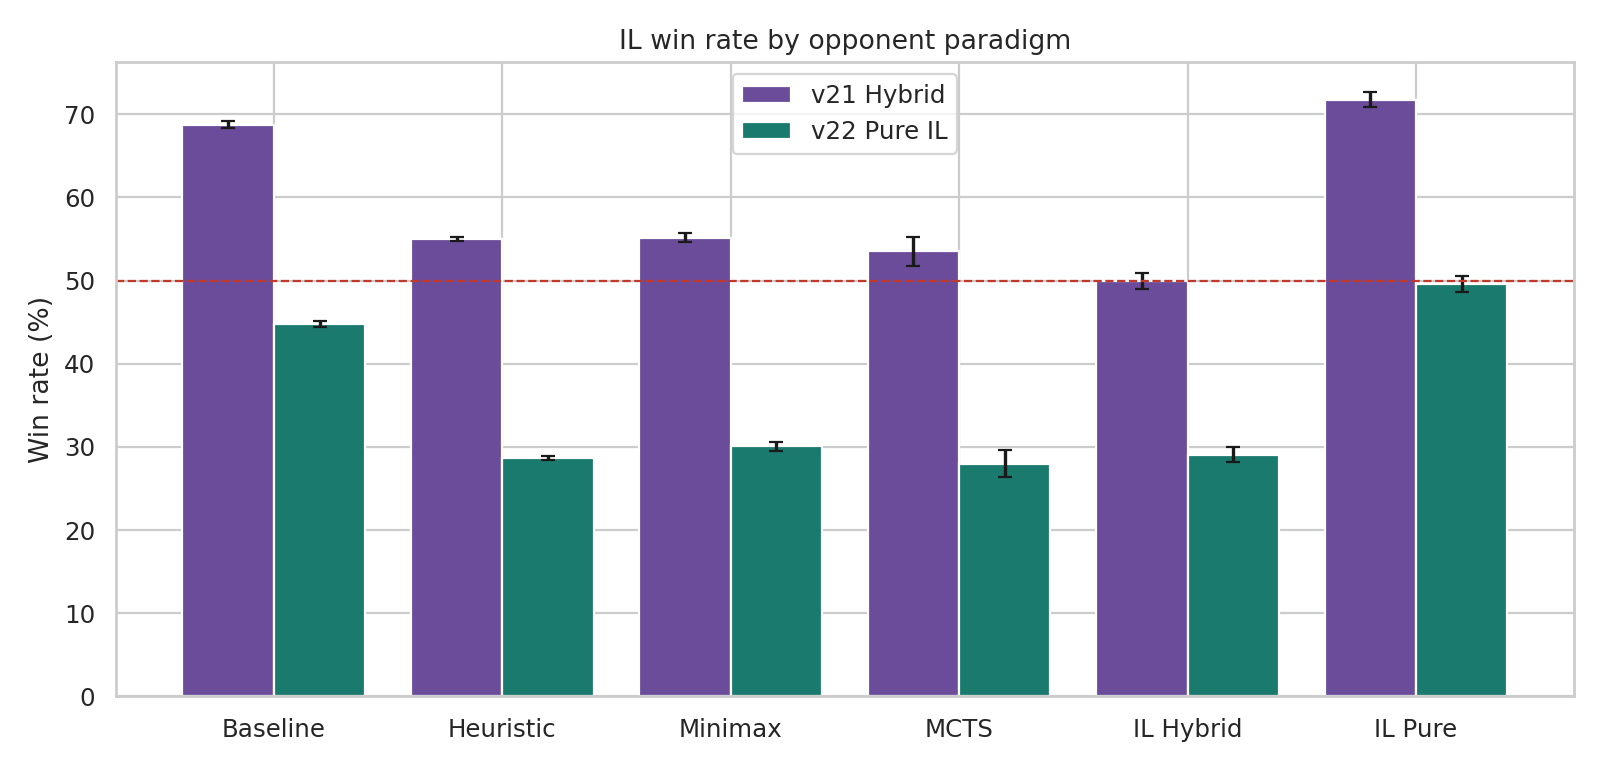
\includegraphics[width=0.92\linewidth]{images/il/il_wr_by_paradigm.png}
    \caption{Taxa de victòries dels agents d'imitació per família d'oponent. \texttt{v21} supera \texttt{v22} en els sis blocs, amb diferències d'aproximadament 20--26~pp.}
    \label{fig:il_paradigm}
\end{figure}

\begin{figure}[htbp]
    \centering
    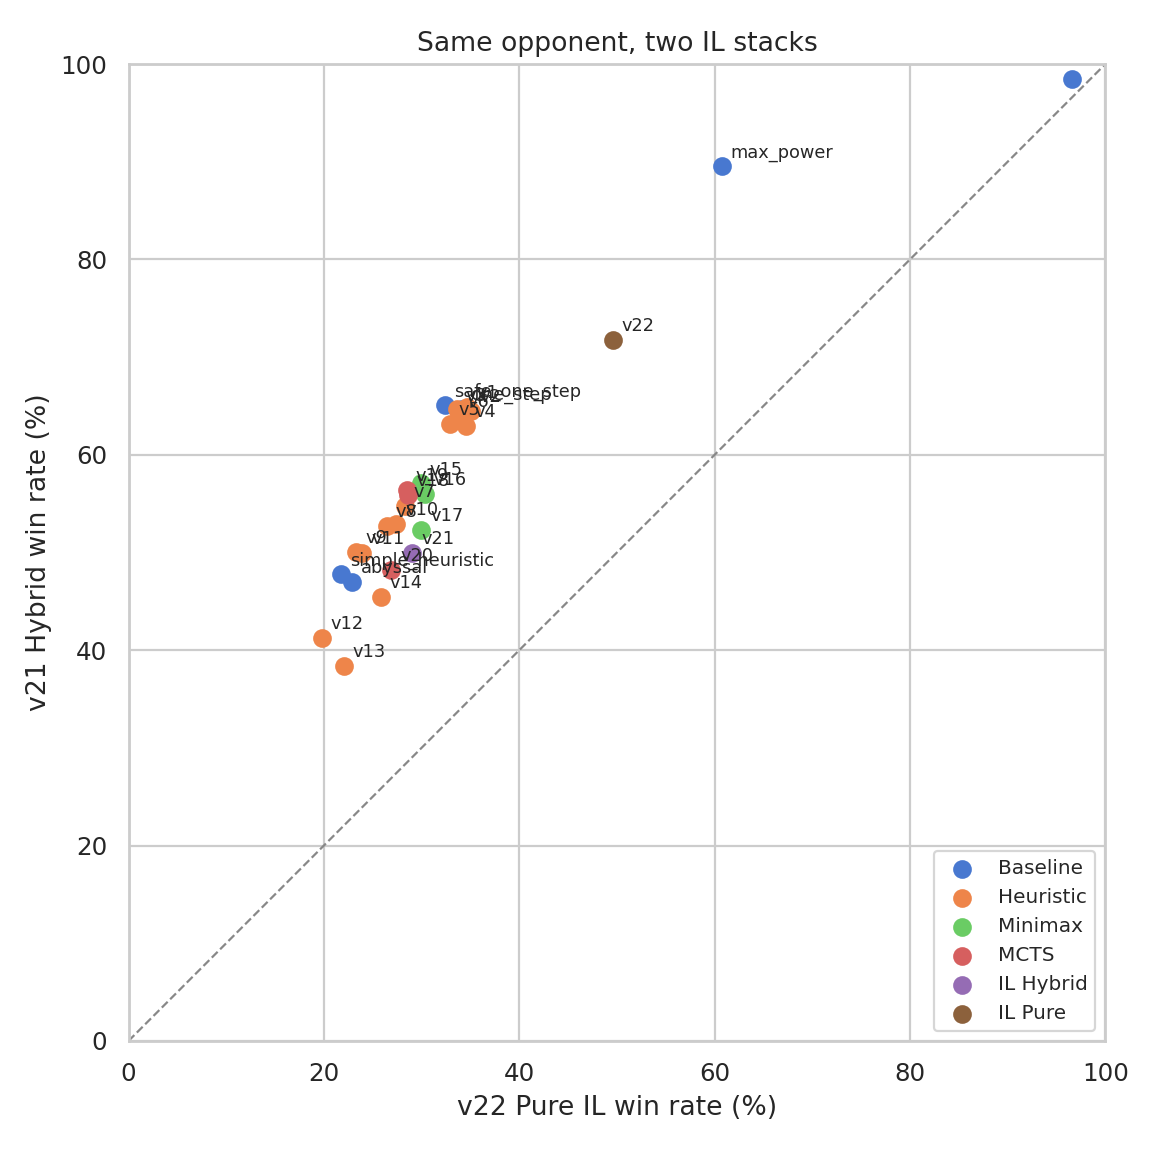
\includegraphics[width=0.85\linewidth]{images/il/il_wr_scatter.png}
    \caption{Taxa de victòries de \texttt{v21} i \texttt{v22} per oponent. Tots els punts queden \emph{per sobre} de la diagonal $y=x$: \texttt{v21} obté el valor superior en 28 de 28 enfrontaments. La diferència màxima és de 32,6~pp contra \texttt{safe\_one\_step}.}
    \label{fig:il_scatter}
\end{figure}

% ============================================================
\FloatBarrier
\section{Comparació entre els cinc paradigmes}
\label{sec:res_cross}

\begin{table}[H]
\centering
\caption{Síntesi dels cinc paradigmes amb \texttt{v12} com a comparador comú. Les variants són les que obtenen el millor resultat observat dins de cada família; aquesta selecció és posterior a l'experiment. L'MCTS té una mostra menor i el PPO no participa en la matriu completa.}
\label{tab:paradigm_summary}
\small
\begin{tabularx}{\textwidth}{llrrX}
\toprule
\textbf{Paradigma} & \textbf{Variant} & \textbf{$n$} & \textbf{vs \texttt{v12}} & \textbf{Lectura} \\
\midrule
Heurístiques & \texttt{v12} & 10.000 & 50,1\% & Autojoc de referència; 59,91\% contra Abyssal. \\
Minimax d'un torn & \texttt{v17} & 10.000 & 40,94\% & El prior cap a \texttt{v14} millora les altres variants, però no supera \texttt{v12}. \\
MCTS ras & \texttt{v20} & 1.000 & 42,7\% & PUCT redueix la discrepància amb \texttt{v14}; marge aproximat de $\pm 3$~pp. \\
Imitació & \texttt{v21} & 10.000 & 41,28\% & El model decideix quan canviar i \texttt{v14} executa l'acció. \\
PPO & model A & 10.000 & 34,1\% & Experiment separat, inicialitzat per clonatge de \texttt{v8}. \\
\bottomrule
\end{tabularx}
\end{table}


La Taula~\ref{tab:paradigm_summary}, juntament amb la Taula~\ref{tab:overall_wr} i la Taula~\ref{tab:vs_disc}, utilitzen comparadors comuns per contrastar els cinc paradigmes. És la comparació més directa disponible per als cinc paradigmes, però no iguala el pressupost de l'MCTS, no controla el cost d'entrenament i selecciona posteriorment la variant amb millor resultat de cada família. Sota aquestes condicions, cap de les implementacions de minimax, MCTS, imitació o PPO arriba al 50\% contra \texttt{v12}.

\begin{table}[H]
\centering
\caption{Taxa de victòries global com a \emph{nosaltres} contra els 28 oponents. Heurístiques, minimax i IL: $253.000$ partides (25 oponents $\times 10.000$ + 3 MCTS $\times 1.000$). MCTS: $28.000$ partides, totes les cel·les amb $n=1.000$. No es poden comparar els dos globals com si tinguessin la mateixa precisió; per ordenar \texttt{v20} contra \texttt{v17} cal mirar cel·les de matchup. Font: \texttt{data/benchmarks/all\_10k/gen9randombattle}.}
\label{tab:overall_wr}
\small
\begin{tabular}{rlrrl}
\toprule
\textbf{Rang} & \textbf{Agent} & \textbf{Partides} & \textbf{WR (\%)} & \textbf{Paradigma} \\
\midrule
1  & \texttt{v12}              & 253.000 & 69,01 & Heurística \\
2  & \texttt{v13}              & 253.000 & 67,63 & Heurística \\
3  & \texttt{v14}              & 253.000 & 62,03 & Heurística \\
4  & \texttt{abyssal}          & 253.000 & 62,00 & Baseline \\
5  & \texttt{simple\_heuristic}& 253.000 & 61,93 & Baseline \\
6  & \texttt{v20}              &  28.000 & 59,66 & MCTS (cel·les $n=1$k) \\
7  & \texttt{v11}              & 253.000 & 59,26 & Heurística \\
8  & \texttt{v9}               & 253.000 & 58,86 & Heurística \\
9  & \texttt{v21}              & 253.000 & 58,71 & IL híbrid \\
10 & \texttt{v17}              & 253.000 & 57,89 & Minimax \\
11 & \texttt{v10}              & 253.000 & 55,66 & Heurística \\
12 & \texttt{v8}               & 253.000 & 55,43 & Heurística \\
13 & \texttt{v16}              & 253.000 & 54,30 & Minimax \\
14 & \texttt{v7}               & 253.000 & 54,25 & Heurística \\
15 & \texttt{v18}              &  28.000 & 54,02 & MCTS (cel·les $n=1$k) \\
16 & \texttt{v15}              & 253.000 & 53,80 & Minimax \\
17 & \texttt{v19}              &  28.000 & 53,29 & MCTS (cel·les $n=1$k) \\
\midrule
-- & \texttt{v5}               & 253.000 & 45,86 & Heurística (altiplà) \\
-- & \texttt{v1}               & 253.000 & 44,25 & Heurística (altiplà) \\
-- & \texttt{v22}              & 253.000 & 33,49 & IL pur \\
-- & \texttt{max\_power}       & 253.000 & 19,66 & Baseline \\
-- & \texttt{random}           & 253.000 &  4,20 & Baseline (àncora Elo $=1000$) \\
\bottomrule
\end{tabular}
\end{table}


\begin{table}[H]
\centering
\caption{Enfrontaments de referència. Les files amb MCTS tenen $n=1.000$ i la resta, $n=10.000$. \texttt{v12} contra Abyssal (59,91\% $\pm 0,96$~pp) és el principal resultat contra un agent extern basat en regles.}
\label{tab:vs_disc}
\small
\begin{tabular}{lrrrr}
\toprule
\textbf{Agent} & \textbf{vs Abyssal} & \textbf{vs \texttt{v12}} & \textbf{vs \texttt{v14}} & \textbf{vs SimpleH} \\
\midrule
\texttt{v12} & 59,91 & 50,1 (autojoc) & 56,01 & 59,75 \\
\texttt{v13} & 55,34 & 48,85 & 57,71 & 56,10 \\
\texttt{v14} & 51,36 & 44,74 & 50,1 (autojoc) & 50,66 \\
\texttt{v20} ($n=1$k) & 49,0 & 42,7 & 47,0 & 49,2 \\
\texttt{v21} & 46,98 & 41,28 & 45,43 & 47,76 \\
\texttt{v17} & 46,79 & 40,94 & 43,61 & 46,75 \\
\texttt{v16} & 41,86 & 35,92 & 39,56 & 40,65 \\
\texttt{v15} & 41,72 & 36,04 & 39,43 & 41,23 \\
\texttt{v18} ($n=1$k) & 42,2 & 34,0 & 40,0 & 42,0 \\
\texttt{v1}  & 30,64 & 23,29 & 32,09 & 30,26 \\
\texttt{v22} & 22,90 & 19,80 & 25,81 & 21,73 \\
\bottomrule
\end{tabular}
\end{table}


\begin{figure}[htbp]
    \centering
    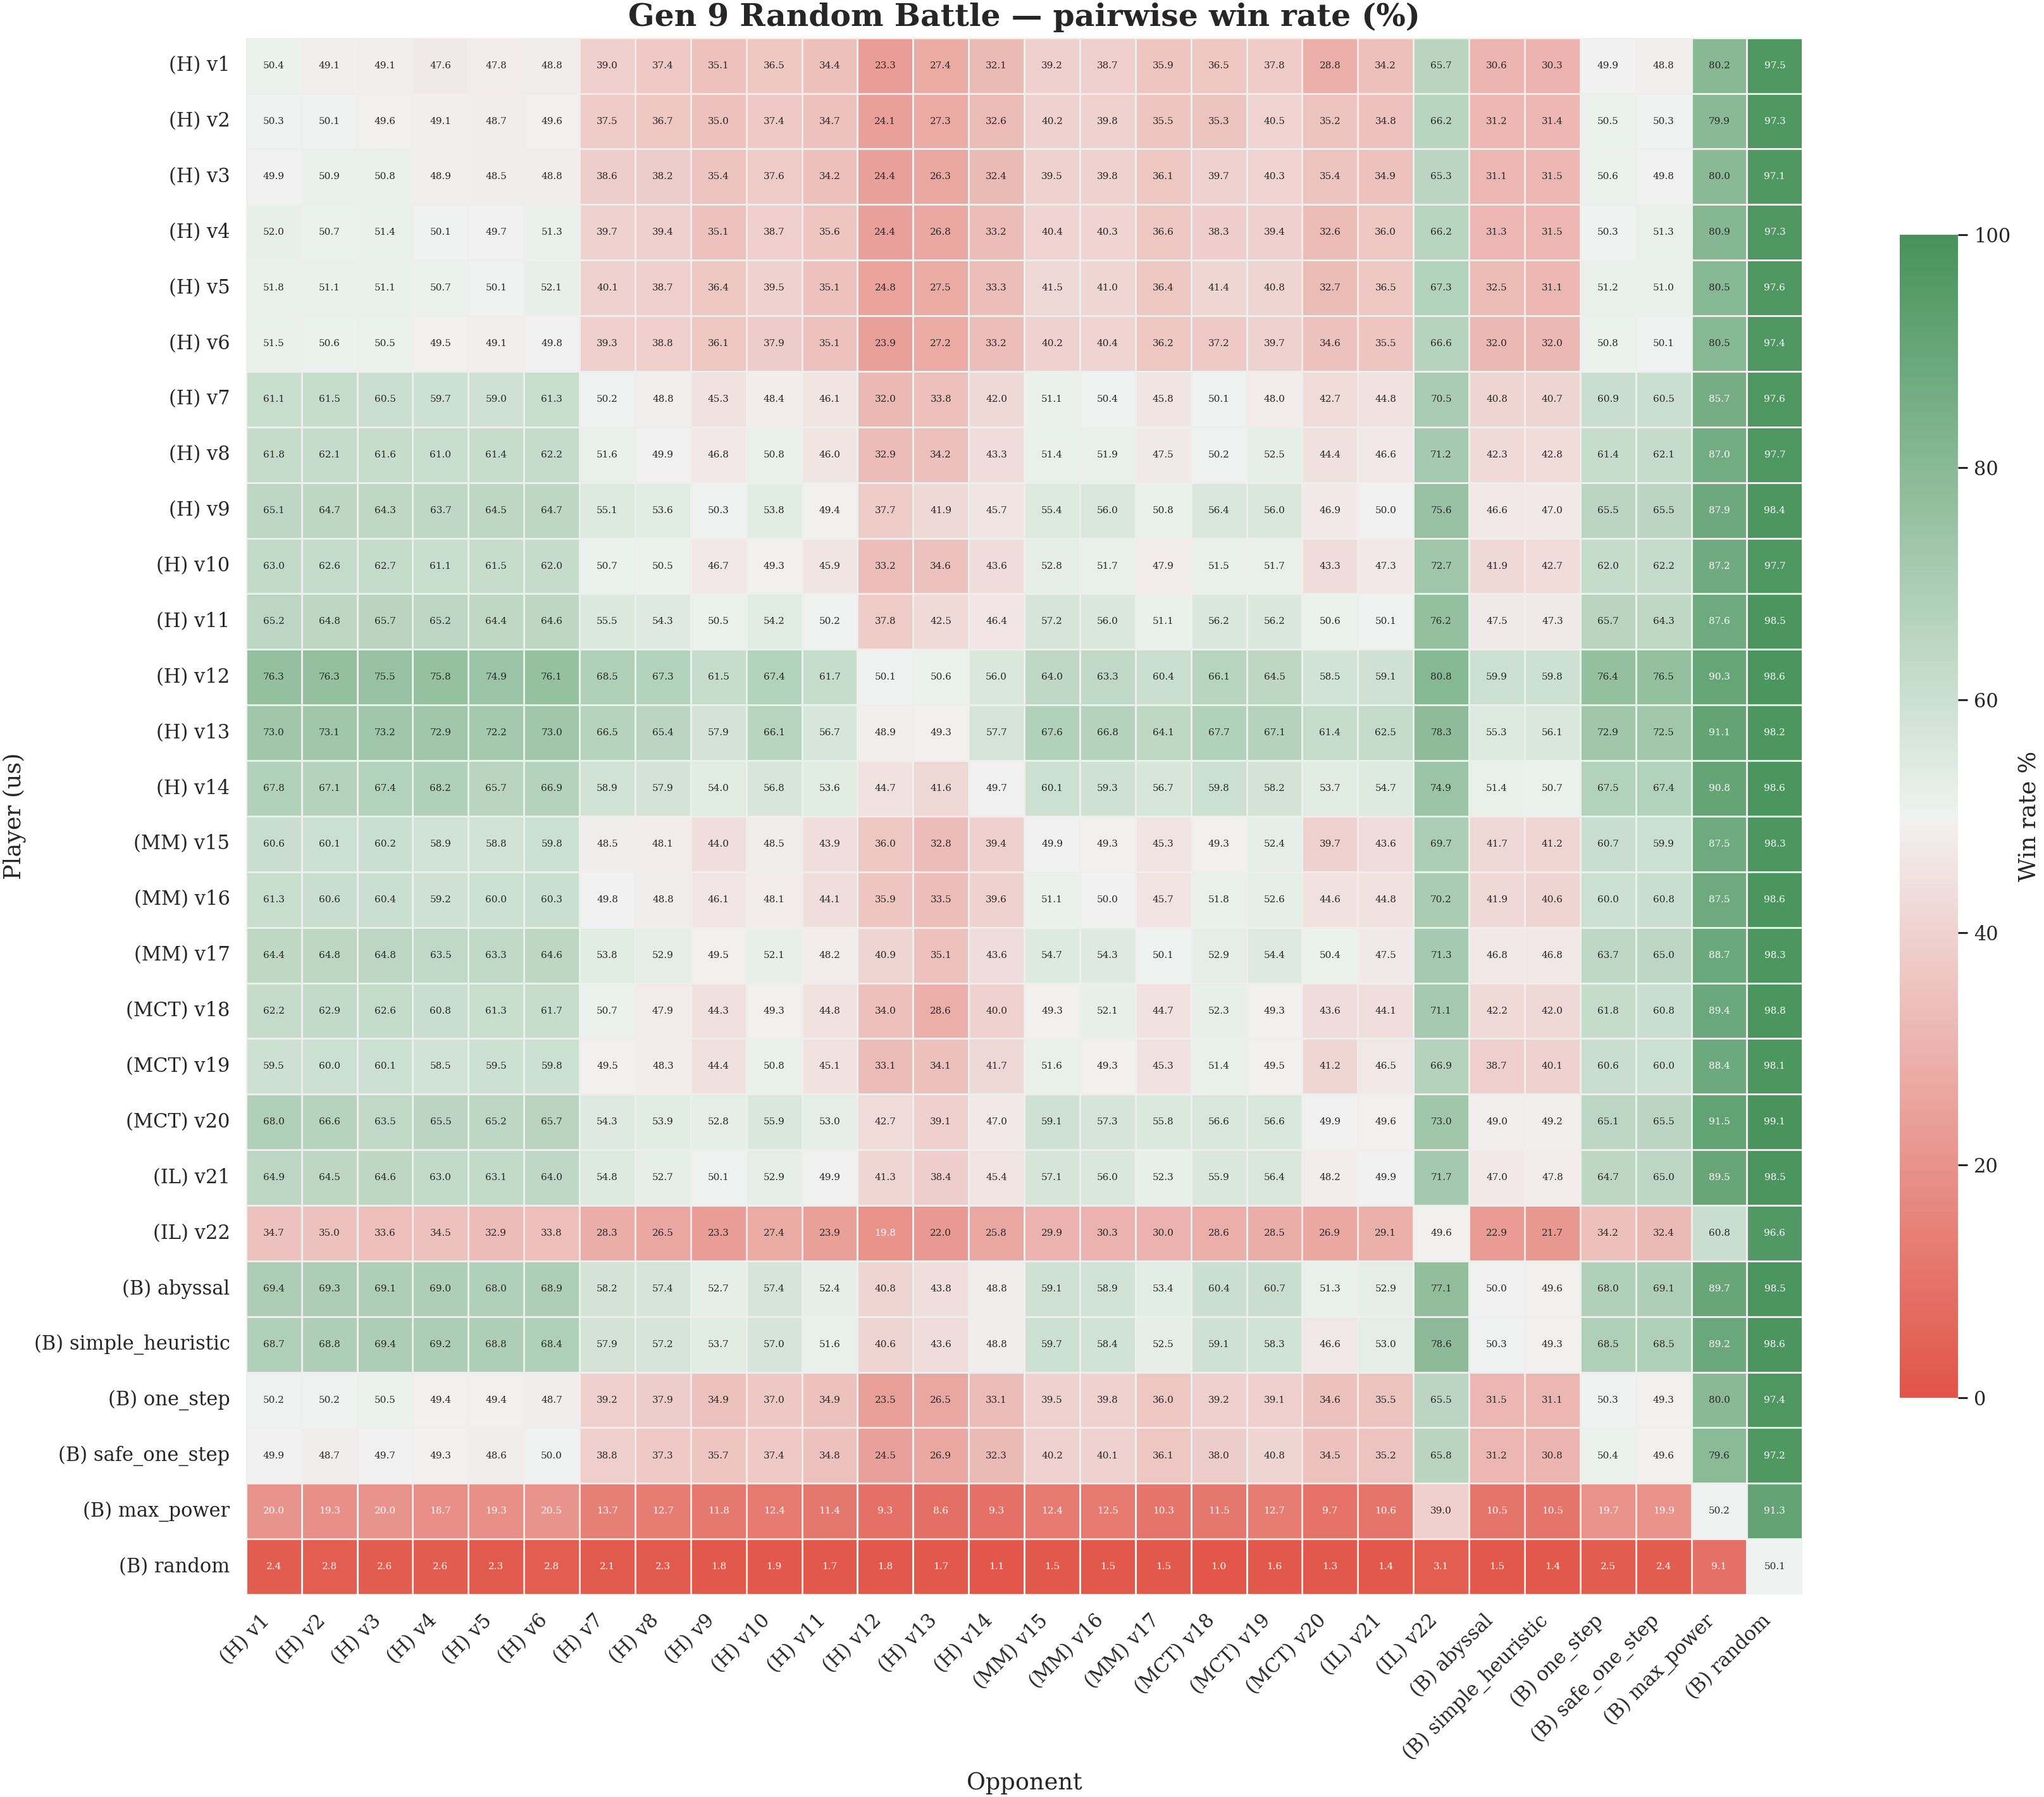
\includegraphics[width=\linewidth]{images/results/gen9_winrate_heatmap.png}
    \caption{Mapa de calor de la taxa de victòries a \texttt{gen9randombattle}. La fila és l'agent analitzat i la columna, l'oponent. Prefixos: (H) heurística, (MM) minimax, (MCT) MCTS, (IL) imitació i (B) agent de referència. Les cel·les amb MCTS tenen $n=1.000$; la resta, $n=10.000$.}
    \label{fig:heatmap}
\end{figure}

\subsection{Abyssal com a agent de referència}

Fins a \texttt{v12}, cap heurística interna supera el 50\% contra Abyssal. \texttt{v7}--\texttt{v11} obtenen entre 41\% i 48\%; \texttt{v12} arriba a 59,91\%. \texttt{v14} obté 51,36\%, \texttt{v21} 46,98\%, \texttt{v20} 49,0\% amb $n=1.000$, \texttt{v17} 46,79\% i \texttt{v22} 22,90\%. El resultat de referència és, per tant, \textbf{\texttt{v12} contra Abyssal: 59,91\% $\pm 0{,}96$~pp, $n=10.000$}.

\subsection{Escala Bradley--Terry}

Com a complement a les taxes directes de victòria per parelles, s'ajusta el model de Bradley--Terry definit a la Secció~\ref{subsec:marc_estadistic} mitjançant regressió logística per màxima versemblança (MLE) sobre la matriu completa de 784 cel·les dirigides, ancorant l'escala a $\text{Random} = 1000$ (Figura~\ref{fig:elo_bars}). Aquesta representació condensa les preferències relatives empíriques en una dimensió latent contínua de força competitiva independent de la composició del calendari d'enfrontaments.

Tal com s'observa a la Figura~\ref{fig:elo_bars}, \texttt{v12} (1812) i \texttt{v13} (1802) assoleixen les puntuacions latents superiors del conjunt, corroborant la seva consistència tant davant d'adversaris d'alt nivell com davant de la resta d'heurístiques. Immediatament per sota, es produeix una convergència al voltant dels 1755 punts entre \texttt{v14} (1755), \texttt{simple\_heuristic} (1755) i Abyssal (1755). Aquesta coincidència numèrica posa de manifest un altiplà competitiu compartit: les tres polítiques basades en regles expertes assoleixen un nivell de domini equivalent sobre el conjunt del ventall, i les diferències decimals entre elles ($<0{,}3$ punts) són estadísticament negligibles.

Pel que fa a la resta de paradigmes, les seves variants més competitives s'estableixen en una franja intermèdia propera: \texttt{v20} (MCTS PUCT, 1742), \texttt{v21} (imitació híbrida XGBoost, 1729) i \texttt{v17} (minimax amb prior, 1722). A la banda inferior de l'escala, \texttt{v22} (imitació pura d'atributs sense proteccions de domini, 1529), \texttt{max\_power} (1383) i \texttt{random} (1000) delimiten la línia de base de l'entorn.

\paragraph{Precaució interpretativa: per què no constitueix una classificació unificada.}
Convé subratllar amb rigor que la Figura~\ref{fig:elo_bars} reflecteix una estimació global de força latent sobre la matriu observada i \textbf{no s'ha d'interpretar com una classificació lineal o un rànquing ordinal absolut}. Aquesta distinció és crítica per tres raons metodològiques:
\begin{enumerate}
    \item \textbf{Asimetria mostral i de pressupost en MCTS:} Mentre que els agents heurístics, minimax, imitació i referència aporten $n=10.000$ partides per cel·la (506.000 partides dirigides per agent al model), les variants d'MCTS (\texttt{v18}--\texttt{v20}) es van avaluar a $n=1.000$ per cel·la (56.000 partides) i sota un pressupost d'inferència estrictament acotat a 5 torns de desplegament. Aquesta diferència de volum mostral implica una variància d'estimació superior que desaconsella intercalar ordinalment MCTS amb la resta d'agents.
    \item \textbf{Precisió asimptòtica i interpretació per estrats:} Gràcies a l'elevat volum de dades (253.000 partides com a fila i el mateix volum com a oponent, 506.000 aparicions per a cada agent no MCTS), l'error estàndard asimptòtic de les estimacions de màxima versemblança és extremadament reduït ($\pm 2$--$3$ punts Elo), fent que la separació entre grans macroestrats (com els 1812 de \texttt{v12} enfront dels 1755 de \texttt{v14}) sigui estadísticament inequívoca. No obstant això, aquesta precisió global no autoritza a proclamar superioritat ordinal \emph{dins} d'un mateix altiplà (com les diferències decimals entre \texttt{v14}, Abyssal i \texttt{simple\_heuristic} a 1755 punts). Per a aquestes comparacions de detall, el treball recorre als intervals de confiança de Wilson al $95\%$ ($\pm 0{,}96$~pp) sobre les taxes directes de victòria per parelles.
    \item \textbf{Intransitivitat i dinàmiques de tipus (pedra-paper-tisores):} Tal com evidencia el mapa de calor dirigit (Figura~\ref{fig:heatmap}) i la inversió d'estils de la Secció~\ref{sec:res_inversion}, l'espai de joc de Pokémon Random Battles presenta cicles intransitius d'especialització que cap projecció unidimensional pot capturar íntegrament sense pèrdua d'informació estructural.
\end{enumerate}
Per aquest motiu, l'anàlisi comparativa interparadigma s'articula fonamentalment a través de l'oponent comú \texttt{v12} (Taula~\ref{tab:paradigm_summary}) i de les taxes agrupades per família (Taula~\ref{tab:overall_wr}), evitant tractar la matriu heterogènia com una lliga única.

\begin{figure}[htbp]
    \centering
    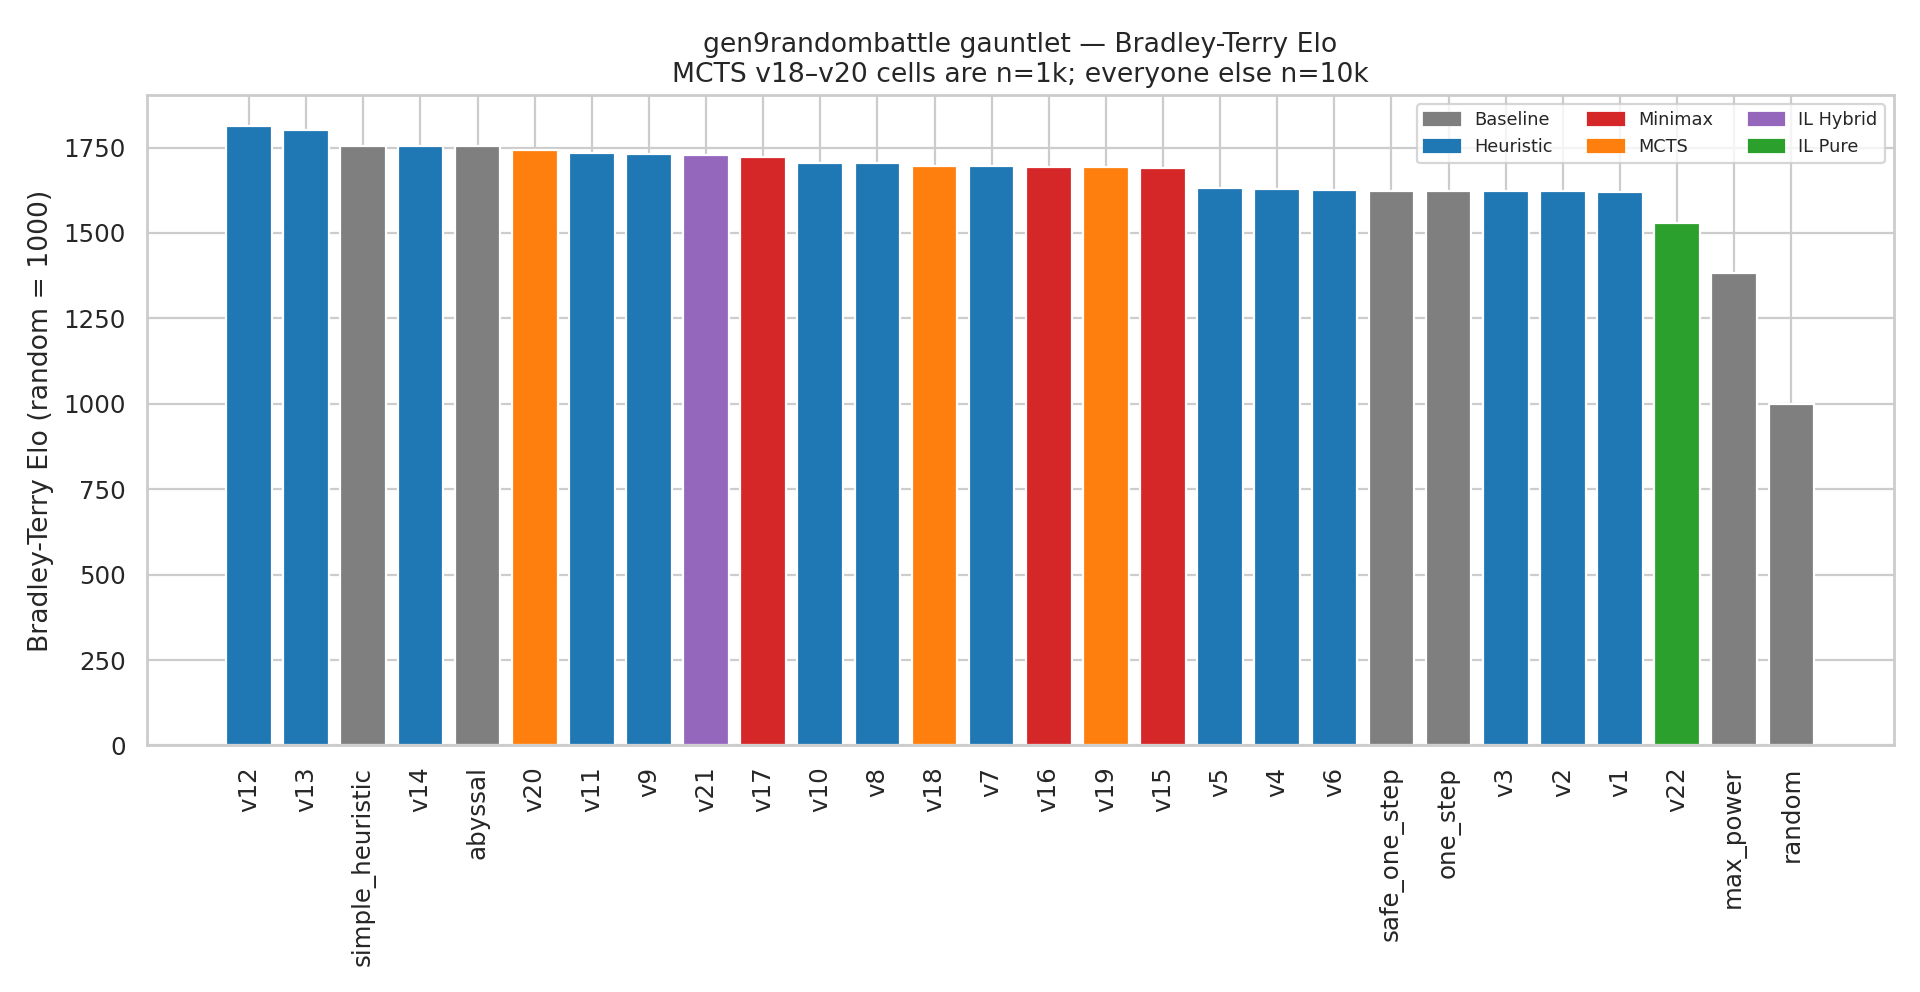
\includegraphics[width=0.92\linewidth]{images/results/gen9_elo_bars.png}
    \caption{Escala latent Bradley--Terry ancorada a \texttt{random}${}=1000$ ajustada sobre les dues orientacions de la matriu. \texttt{v12} i \texttt{v13} obtenen les puntuacions més altes; \texttt{v14}, Abyssal i Simple Heuristic comparteixen un altiplà a 1755 punts. Les files i columnes d'MCTS aporten una desena part de partides al model ($n=1.000$).}
    \label{fig:elo_bars}
\end{figure}

% ============================================================
\FloatBarrier
\section{Classificació pública: avaluació exploratòria de \texttt{v14}}
\label{sec:res_ladder}

\begin{table}[H]
\centering
\caption{Ladder pública de \texttt{v14} contra humans (\texttt{gen9randombattle}, usuari \texttt{SirPThesis}, 9--10 de juny de 2026). Font: \texttt{data/testing/logs/logs\_v14\_online/battle\_history.csv}. El snapshot del pla de juny (98 partides, 40,8\%, Elo $\sim$1151) és un \emph{prefix} d'aquest mateix log, pres a prop del pic d'Elo: no és la mostra final.}
\label{tab:ladder_v14}
\small
\begin{tabular}{lr}
\toprule
\textbf{Mètrica} & \textbf{Valor} \\
\midrule
Partides úniques acabades & 431 \\
Victòries & 170 / 431 \\
WR en brut & 39,44\% $\pm 4{,}6$~pp \\
Només torns $\ge 10$ (taules tàctiques) & 35,43\% ($n=398$) \\
Partides curtes (torns $<10$) & 33 (sobretot abandons; inflen el WR brut) \\
Elo & $1085 \rightarrow 1038$ (rang $1000$--$1263$) \\
Errors / fallbacks & 0 / 13 \\
Finestra & 2026-06-09 21:54 -- 2026-06-10 18:32 \\
\bottomrule
\end{tabular}
\end{table}


A la classificació pública oficial (\emph{ladder}), \texttt{v14} va disputar 431 partides entre el 9 i el 10 de juny de 2026, assolint una taxa global del 39,44\% $\pm 4,6$~pp (Taula~\ref{tab:ladder_v14} i Figura~\ref{fig:ladder_wr}).

\begin{figure}[htbp]
    \centering
    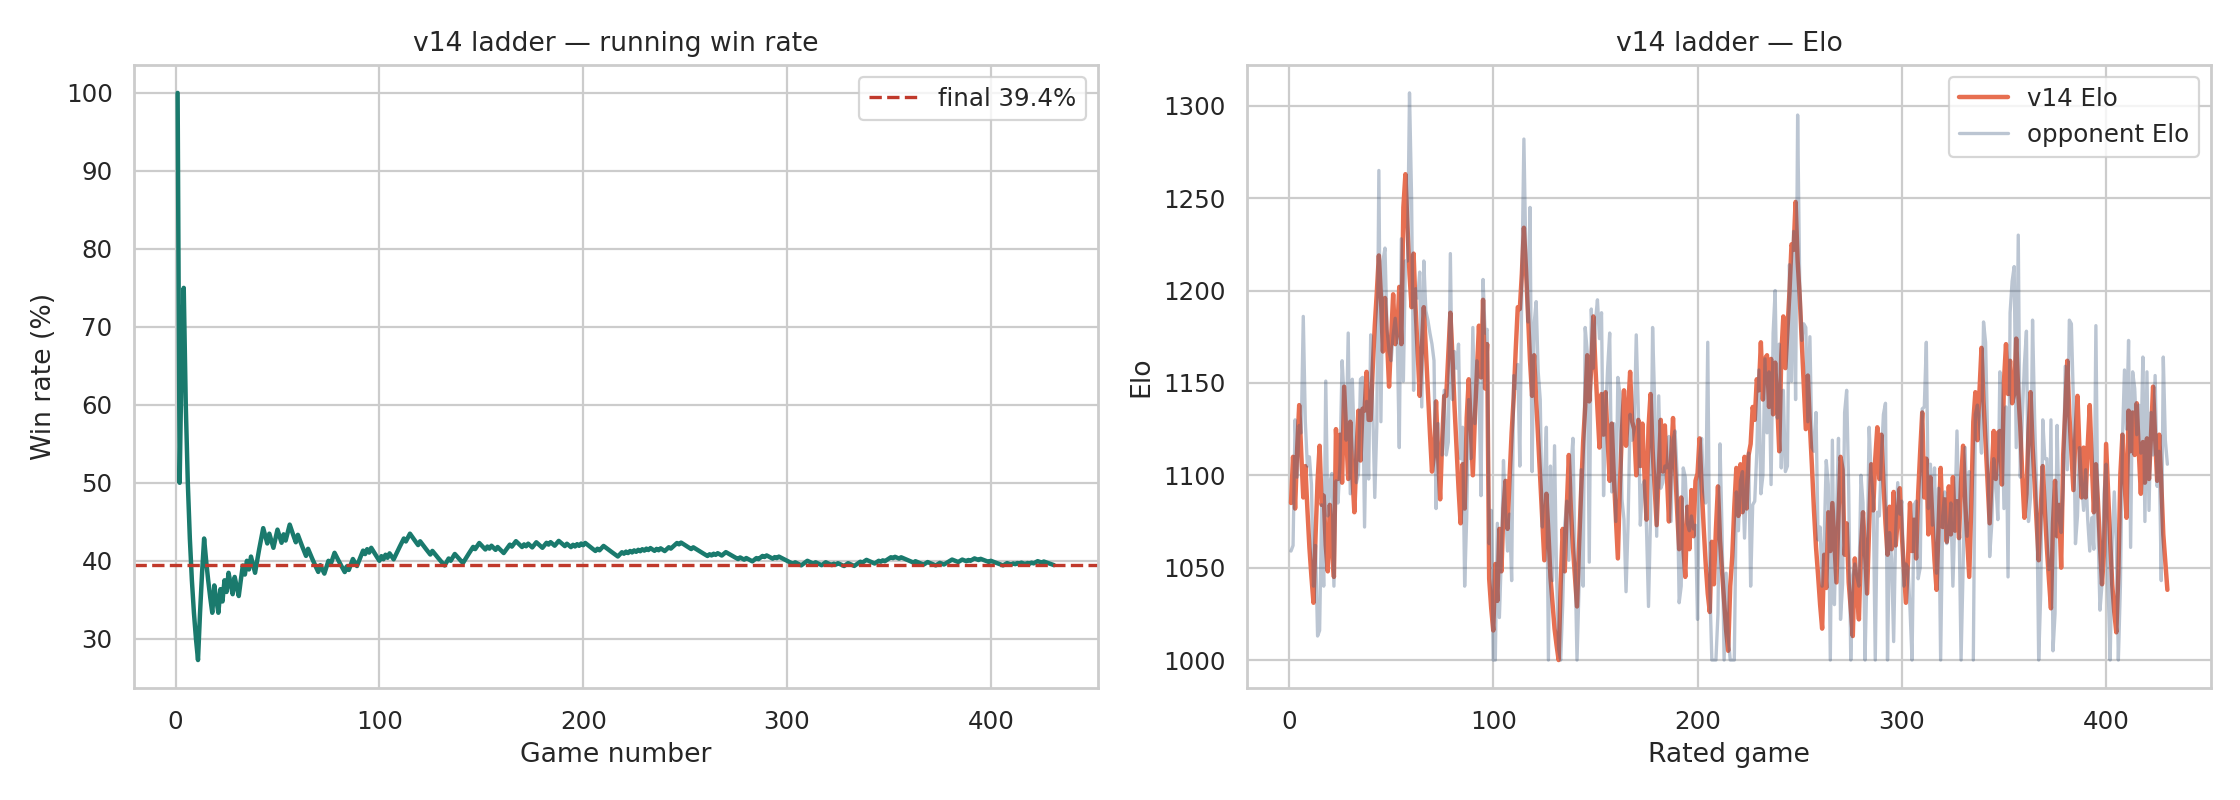
\includegraphics[width=0.92\linewidth]{images/results/ladder_wr_elo.png}
    \caption{Taxa de victòries acumulada i Elo de \texttt{v14} a la classificació pública: 431 partides entre el 9 i el 10 de juny de 2026, 39,44\% $\pm 4,6$~pp i Elo de 1085 a 1038 (màxim 1263). Una instantània prefixa de 98 partides, presa prop del màxim d'Elo, no representa el resultat final.}
    \label{fig:ladder_wr}
\end{figure}

\begin{figure}[htbp]
    \centering
    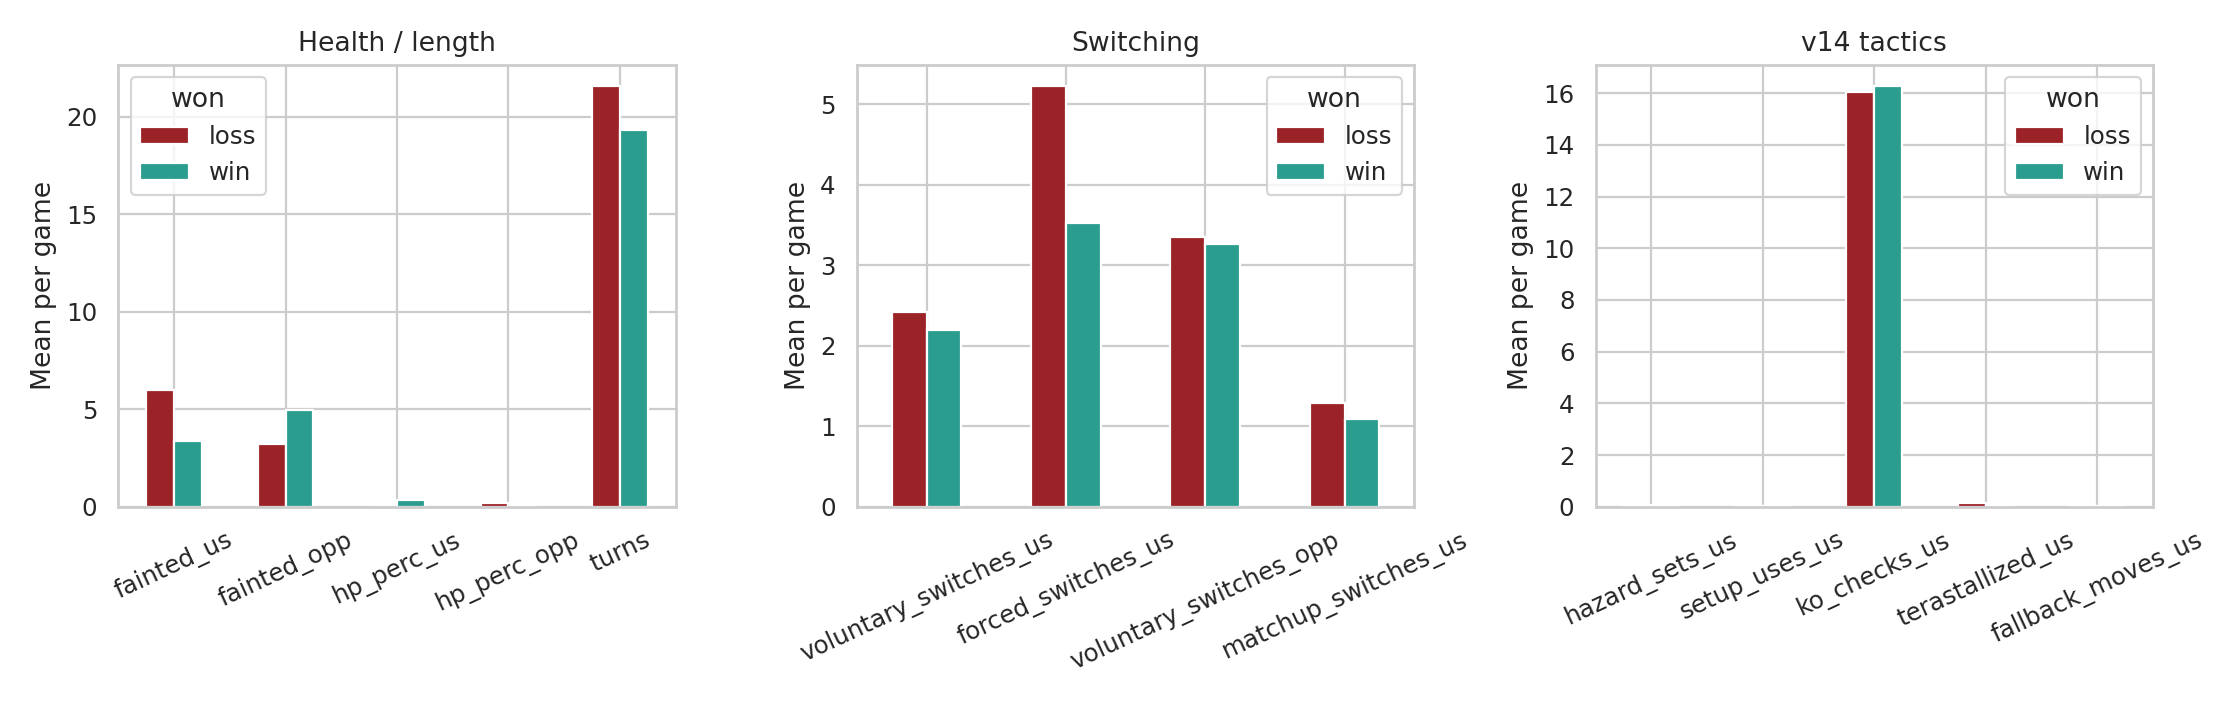
\includegraphics[width=0.92\linewidth]{images/results/ladder_win_vs_loss.png}
    \caption{Telemetria de \texttt{v14} al \emph{ladder}, separada per victòria i derrota: durada i membres debilitats, canvis, i tàctiques (\texttt{ko\_checks} $\sim$16 per partida; preparació, perills i Teracristal·lització molt baixos). El perfil tàctic s'assembla al de la matriu local.}
    \label{fig:ladder_wl}
\end{figure}

En les partides d'almenys 10 torns, \texttt{v14} utilitza la Teracristal·lització en 45 de 398 combats i obté un 20\% de victòries en aquest subconjunt. La telemetria comparativa entre victòries i derrotes (Figura~\ref{fig:ladder_wl}) mostra que presenta moltes comprovacions de debilitament i pocs moviments de preparació, un perfil semblant al de la matriu local. Com que la durada és posterior a les decisions i està relacionada amb el resultat, la taxa filtrada no s'interpreta com una estimació alternativa de rendiment.

Aquesta avaluació pública té un caràcter \textbf{exploratori i anecdòtic}: demostra que el sistema funciona i és capaç de competir en un entorn real amb jugadors humans, però no constitueix una validació estadísticament rigorosa. Amb només 431 partides i una taxa de desconnexions significativa, la mostra és insuficient per a una estimació d'Elo estable. A més, la complexitat matemàtica del domini ---equips aleatoris amb centenars de variables ocultes, com s'ha formalitzat als Capítols~\ref{chap:marc_teoric} i~\ref{chap:metodologia}--- exigeix un volum de partides molt superior per obtenir intervals de confiança acceptables contra oponents no controlats. La selecció d'oponents no està controlada i la mostra no permet inferir el rendiment que hauria obtingut \texttt{v12}.

% ============================================================
\FloatBarrier
\section{PPO contra \texttt{v12}}
\label{sec:res_ppo}

El cinquè paradigma s'avalua fora de la matriu, contra \texttt{v12}, amb $n=10.000$ i les dues orientacions (Secció~\ref{sec:disseny_experiments}). L'entorn, la màscara \texttt{Discrete(14)}, el vector de 328 dimensions i el clonatge de \texttt{v8} (400 partides) són els del Capítol~\ref{chap:implementacio}. Aquí es llegeixen les validacions congelades i el model A.

\begin{table}[htbp]
\centering
\caption{Currículum i avaluacions de MaskablePPO. Els artefactes i hiperparàmetres d'entrenament es detallen a la Taula~\ref{tab:ppo_curriculum_impl}. El resultat principal correspon al model A contra \texttt{HeuristicV12} ($n=10.000$ i ambdues orientacions). La fase~4 només informa de la taxa interna durant l'entrenament, no d'una avaluació independent.}
\label{tab:ppo_head}
\label{tab:ppo_curriculum_eval}
\small
\renewcommand{\arraystretch}{1.15}
\begin{tabularx}{\textwidth}{llrrl>{\raggedright\arraybackslash}X}
\toprule
\textbf{Fase} & \textbf{Oponent} & \textbf{$n$} & \textbf{TV (\%)} & \textbf{Porta de pas} & \textbf{Estat / Observacions} \\
\midrule
1 & Random & 1.000 & 91,8 & $\ge 90\%$ & Superada (graduació) \\
1.5 & MaxBP & 1.000 & 70,5 & $>70\%$ & Superada per estimació puntual \\
2 & \texttt{v8} & 1.000 & 40,6 & $>55\%$ & No superada \\
\textbf{3 (resultat)} & \textbf{\texttt{v12}} & \textbf{10.000} & \textbf{34,1} & --- & Mesura final model A (328 dims, $\pm 0{,}93$~pp) \\
3B (diagnòstic) & \texttt{v12} & 1.000 & 32,6 & --- & Model B, taxa $1{,}5\times10^{-4}$ \\
4 (interrompuda) & \texttt{v12} & 12.554 & 33,5 & --- & Taxa d'entrenament (346 dims, clonatge \texttt{v14}) \\
Control & Random & 1.000 & 98,3 & --- & Verificació d'accions legals (model A) \\
Matriu (context) & \texttt{v8} vs \texttt{v12} & 10.000 & 32,9 & --- & Rendiment del professor de clonatge \\
\bottomrule
\end{tabularx}
\end{table}


\subsection{Resultat principal}

Per avaluar la robustesa del resultat, es van executar \textbf{5 entrenaments independents} amb llavors aleatòries diferents, mantenint la mateixa arquitectura, observació i currículum. El model A (\texttt{p3\_v12\_lr5e5\_flat.zip}) és representatiu del rendiment mitjà del conjunt.

La taxa de victòries mitjana de les 5 execucions contra \texttt{HeuristicV12} és:

\begin{center}
\textbf{34,1\%} \quad $\pm 0{,}93$~pp \quad (IC $\sim$33,2--35,0\%), \quad $\bar{x} = 34{,}1\%$, $\sigma = 0{,}7$~pp.
\end{center}

Les cinc llavors obtenen taxes entre 33,2\% i 34,9\%, confirmant l'estabilitat del resultat. Per orientació, el model A obté 34,2\% (1709/5000) com a p1 i 33,9\% (1696/5000) com a p2, amb 17,2 torns de mitjana. En el control contra Random, la mitjana de les 5 execucions és de \textbf{98,3\%} amb $n=1.000$. Això confirma que la política produeix accions legals i eficaces contra un agent aleatori, però cap de les cinc execucions no arriba al 50\% contra \texttt{v12}.

A la matriu, \texttt{v8} obté \textbf{32,9\%} contra \texttt{v12} ($n=10.000$). La diferència puntual respecte de la mitjana PPO és d'1,2~pp i els intervals se superposen en totes cinc llavors; per tant, no hi ha evidència clara que el model final superi el seu professor de clonatge en aquest comparador.

\subsection{Currículum}

La Taula~\ref{tab:ppo_head} i la Figura~\ref{fig:ppo_curriculum_curves} separen artefactes d'entrenament (Capítol~\ref{chap:implementacio}) i validació congelada. Les dues primeres etapes compleixen el criteri operatiu; la fase~2 no, i la fase~3 s'executa com a prova de continuació.

No és correcte descriure el currículum com quatre graduacions reeixides. Una configuració amb taxa $1{,}5\times 10^{-4}$ i 16 entorns obté 32,6\% contra \texttt{v12} amb $n=1.000$. L'extensió a 346 dimensions, inicialitzada amb \texttt{v14}, es va interrompre amb una taxa d'entrenament aproximada del 33,5\%. Aquests valors són diagnòstics i no substitueixen l'avaluació del model A.

\subsection{Interpretació del límit observat}

Hi ha diverses explicacions compatibles amb el 34,1\%, però les dades no permeten triar-ne una de manera causal:

\begin{enumerate}
    \item \textbf{Professor inicial.} El clonatge parteix de \texttt{v8}, que obté 32,9\% contra \texttt{v12}. El resultat final és proper a aquest punt de partida.
    \item \textbf{Salt de dificultat.} La política no arriba a paritat amb \texttt{v8} abans de passar a \texttt{v12}; per tant, la fase següent comença sense haver consolidat l'anterior.
    \item \textbf{Observació sense memòria.} El vector resumeix l'estat actual, però la política no és recurrent i pot perdre informació temporal útil sobre moviments revelats o patrons del rival.
    \item \textbf{Recompensa modelada.} HP, debilitaments, modificadors i perills proporcionen senyal dens, però poden premiar estats intermedis que no maximitzen la victòria final.
    \item \textbf{Variabilitat d'entrenament.} Les cinc llavors independents mostren una desviació estàndard de 0,7~pp, cosa que suggereix que el límit observat és robust a la inicialització, però no descarta que una configuració d'hiperparàmetres diferent obtingui un resultat substancialment millor.
\end{enumerate}

Amb aquesta observació, recompensa, inicialització i pressupost, cap de les cinc execucions de MaskablePPO no supera \texttt{v12}. La conclusió es limita al sistema executat, no a PPO en general. El resultat més informatiu és que vèncer Random no prediu l'èxit contra una heurística amb coneixement de posició i mecàniques de format.

% ============================================================
\FloatBarrier
\section{Discussió}
\label{sec:res_disc}

\subsection{Patró d'integració residual}

\texttt{v21} (imitació), \texttt{v17} (minimax) i \texttt{v20} (MCTS) comparteixen un patró: conserven les regles tàctiques de \texttt{v14} i hi afegeixen un mòdul que intervé en una fracció de les decisions (Taula~\ref{tab:residual_integration}). Dins de cada família, aquestes variants obtenen un resultat superior a les alternatives que substitueixen més sovint la proposta de \texttt{v14}. PPO, en canvi, no hereta l'executor \texttt{v14} i queda al nivell del professor \texttt{v8}.

\begin{table}[htbp]
    \centering
    \caption{Integració residual sobre \texttt{v14}. El percentatge de torns és la fracció en què s'executa el mòdul afegit; la discrepància és la taxa en què aquest mòdul no retorna l'acció de \texttt{v14} (no aplica a XGBoost ni a PPO). $n=10.000$ tret de \texttt{v20} ($n=1.000$).}
    \label{tab:residual_integration}
    \small
    \renewcommand{\arraystretch}{1.2}
    \begin{tabularx}{\textwidth}{lXccc}
        \toprule
        \textbf{Variant} & \textbf{Mòdul} & \textbf{Torns} & \textbf{Discrepància} & \textbf{vs \texttt{v12}} \\
        \midrule
        \texttt{v17} & maximin d'un torn & 16,3\% & 36,6\% & 40,94\% \\
        \arrayrulecolor{gray!30}\hline\arrayrulecolor{black}
        \texttt{v20} & PUCT, prior $0{,}70$ & 15,5\% & 18,7\% & 42,7\% \\
        \arrayrulecolor{gray!30}\hline\arrayrulecolor{black}
        \texttt{v21} & XGBoost atacar/canviar & 15\% & --- & 41,28\% \\
        \arrayrulecolor{gray!30}\hline\arrayrulecolor{black}
        PPO A & política neuronal & 100\% & --- & 34,1\% \\
        \bottomrule
    \end{tabularx}
\end{table}

El patró no demostra que qualsevol arquitectura híbrida sigui superior. Les variants difereixen en més d'un component i s'han seleccionat després d'observar els resultats. Sí que aporta evidència consistent que, amb les representacions i pressupostos implementats, preservar restriccions tàctiques de domini és important.

\subsection{Resposta conjunta a la pregunta de recerca}

\begin{enumerate}
    \item La seqüència heurística mostra increments associats a posició, control del ritme i mecàniques de Generació~IX. \texttt{v12} obté el millor resultat observat ($69{,}01\%$). El contrast amb \texttt{v13} ---mateixa selecció de substitut, Teracristal·lització reduïda un 79\%--- només retrocedeix $\approx 1{,}4$~pp ($67{,}63\%$) i el duel directe no separa les dues polítiques; això suggereix, com a hipòtesi observacional, que el gruix del salt \texttt{v11}$\to$\texttt{v12} s'associa al substitut informat, no a un efecte causal aïllat de la Tera.
    \item El minimax d'un torn i l'MCTS ras no superen \texttt{v12}. Les millors variants són les que es mantenen més a prop de \texttt{v14}.
    \item El model d'imitació aporta una decisió d'alt nivell aprofitable quan \texttt{v14} executa l'acció. L'execució basada en atributs de \texttt{v22} queda clarament per sota.
    \item MaskablePPO obté 34,1\% contra \texttt{v12}, un resultat proper al de \texttt{v8} contra el mateix oponent i insuficient per afirmar una millora sobre el professor de clonatge.
    \item En el comparador comú \texttt{v12}, cap de les implementacions seleccionades de minimax, MCTS, imitació o PPO arriba al 50\%.
\end{enumerate}

\subsection{Limitacions específiques dels resultats}

\begin{itemize}
    \item Les taxes globals inclouen oponents fàcils, autojoc i etiquetes duplicades, i la ponderació difereix entre files MCTS i no MCTS.
    \item La telemetria heurística de les figures d'aquesta secció és la mitjana ponderada de la matriu completa (253.000 partides per fila); la de minimax, MCTS i imitació també cobreix tota la matriu.
    \item \texttt{endgame\_solves} de \texttt{v18} pot incloure activitat de la sonda \texttt{v14} posterior a la cerca.
    \item \texttt{LocalSim} no és el mateix motor que Showdown; un desajust de mecàniques pot introduir soroll en les simulacions.
    \item L'avaluació pública de \texttt{v14} és una mostra no controlada de 431 partides.
    \item El PPO només es compara amb \texttt{v12}; les cinc llavors confirmen l'estabilitat del resultat, però no s'ha explorat una cerca d'hiperparàmetres més àmplia.
\end{itemize}

% !TEX root = ../main.tex
\chapter{Conclusions i línies futures}
\label{chap:conclusions}

\section{Resposta a la pregunta de recerca}

La pregunta que vertebra el treball és aquesta: \emph{sota un mateix simulador, format i protocol, quin dels cinc paradigmes ---heurístiques, minimax d'un torn, MCTS ras, imitació i MaskablePPO--- obté millor rendiment observat a \texttt{gen9randombattle}, i què explica les diferències?}

Heurístiques, minimax, MCTS ras i imitació, amb sis agents de referència, formen una matriu dirigida de $28\times 28$. MaskablePPO s'avalua a part, contra \texttt{v12}. La comparació comparteix Showdown i el format, però no és simètrica: l'MCTS té $n=1.000$ per cel·la i el PPO no entra a la lliga.

Resposta: sota les implementacions i els pressupostos d'aquest experiment, les heurístiques obtenen el millor resultat observat. \texttt{v12} assoleix 69,01\% de mitjana global descriptiva i 59,91\% contra Abyssal. Contra el mateix comparador \texttt{v12}, \texttt{v17} (minimax) obté 40,94\%, \texttt{v20} (MCTS) 42,7\%, \texttt{v21} (imitació) 41,28\% i el model PPO 34,1\% ($n=10.000$ tret de l'MCTS).

Això no afirma que les heurístiques siguin universalment superiors. Afirma que, aquí, el coneixement explícit sobre Teracristal·lització, selecció del substitut, debilitaments garantits i control del ritme no el recuperen ni la cerca rasa ni els models apresos amb els recursos utilitzats.

\subsection{Grau d'acompliment dels objectius específics}

A partir dels resultats empírics obtinguts, es pot verificar el compliment dels sis objectius específics plantejats en la Introducció (Secció~\ref{sec:objectius}):

\begin{enumerate}
    \item \textbf{Formalització teòrica del domini (Acomplert):} S'ha formalitzat el combat Pokémon com un joc estocàstic parcialment observable de dos jugadors (POSG) al Capítol~\ref{chap:marc_teoric}, i s'ha justificat la reducció a POMDP quan un sol decisor absorbeix la política rival $\pi_2$ dins de $T$. S'han definit les fonts d'incertesa de l'estat ocult, la dinàmica d'accions simultànies i les transicions estocàstiques.
    \item \textbf{Disseny metodològic, infraestructura i telemetria (Acomplert):} S'ha dissenyat el protocol experimental i el model de rànquing Bradley--Terry (Capítol~\ref{chap:metodologia}), s'ha construït la infraestructura computacional paral·lela i recuperable (Capítol~\ref{chap:infraestructura}) que ha produït 6.409.000 batalles dirigides a la matriu, i s'ha instrumentat el marc de telemetria per torn per a l'explicabilitat conductual.
    \item \textbf{Paradigmes heurístics i de cerca en línia (Acomplert):} S'ha desenvolupat la seqüència d'ablacions heurístiques (\texttt{v1}--\texttt{v14}) i s'han implementat i instrumentat les variants de cerca minimax d'un torn (\texttt{v15}--\texttt{v17}) i MCTS ras (\texttt{v18}--\texttt{v20}) amb priors d'orientació (Capítol~\ref{chap:implementacio}). \texttt{v12} és la millor heurística observada; \texttt{v14} és l'heurística de servei (fulla, prior PUCT, executor d'imitació i bot del \emph{ladder}).
    \item \textbf{Agents apresos i integració de LLMs (Acomplert):} S'han entrenat els models d'imitació XGBoost (\texttt{v21}--\texttt{v22}), s'ha optimitzat MaskablePPO amb clonatge conductual sobre \texttt{v8} i s'ha avaluat la viabilitat exploratòria de \textit{PokéChamp} i \textit{PokéLLMon}.
    \item \textbf{Avaluació empírica massiva i rànquings (Acomplert):} S'ha completat l'avaluació de la matriu competitiva dirigida de 28 agents ($28\times 28$), calculant els rànquings Bradley--Terry i analitzant el comportament obtingut per telemetria (Capítol~\ref{chap:resultats}).
    \item \textbf{Avaluació externa al ladder públic (Acomplert):} S'ha desplegat l'heurística de servei (\texttt{v14}) a la classificació pública de Pokémon Showdown, amb 431 batalles contra jugadors humans (usuari \texttt{SirPThesis}). El desplegament no pretén que \texttt{v14} sigui l'agent de millor taxa; és la política més completa i instrumentada per operar en línia.
\end{enumerate}

\section{Resultats principals i avaluació de les hipòtesis}
\label{sec:resultats_principals_hipotesis}

A continuació es contrasten els resultats empírics amb les cinc hipòtesis de recerca formalitzades a la Secció~\ref{subsec:hipotesis}:

\begin{enumerate}
    \item \textbf{$\mathbf{H_1}$ (Monotonicitat de l'ablació heurística) --- Refutada: La complexitat heurística no produeix una millora monotònica.} \texttt{v1}--\texttt{v6} formen un altiplà d'efectivitat similar; \texttt{v7}, \texttt{v9} i \texttt{v12} introdueixen els salts de rendiment més rellevants. Tanmateix, les versions més complexes (\texttt{v13} i \texttt{v14}) afegeixen una càrrega de regles que, lluny de millorar el joc, redueix la taxa global (62,03\% per a \texttt{v14} enfront del 69,01\% de \texttt{v12}), compatible amb una especialització de domini (més inferència i model de rival) que no ajuda contra polítiques deterministes.
    \item \textbf{$\mathbf{H_2}$ (Cerca adversària en línia) --- Refutada: El minimax d'un torn i l'MCTS ras no superen l'heurística de partida.} Ni la matriu simultània minimax (\texttt{v15}--\texttt{v17}) ni les simulacions locals MCTS a cinc torns (\texttt{v18}--\texttt{v20}) aconsegueixen batre la política que avalua les fulles (\texttt{v14}) ni l'heurística òptima (\texttt{v12}). \texttt{v17} obté un 43,61\% contra \texttt{v14} i un 40,94\% contra \texttt{v12}, mentre que \texttt{v20} n'obté un 42,7\%. La incertesa de l'estat ocult rival i el soroll estocàstic limiten la utilitat de la cerca a poca profunditat.
    \item \textbf{$\mathbf{H_3}$ (Guiatge per priors a l'MCTS) --- Confirmada: L'MCTS ras depèn críticament del biaix heurístic.} La cerca sense informació prèvia (UCB1) discrepa de les decisions expertes de \texttt{v14} en el 71,3\% de les decisions de cerca (\texttt{v18}), generant branques subòptimes. La incorporació de priors heurístics mitjançant l'algorisme PUCT redueix aquesta taxa de discrepància dràsticament al 18,7\% i millora la puntuació Bradley--Terry de la família (1742 per a \texttt{v20} vs. 1697 per a \texttt{v18}).
    \item \textbf{$\mathbf{H_4}$ (Bastida de domini a la imitació) --- Confirmada: La imitació requereix regles expertes d'execució.} L'agent híbrid \texttt{v21} (XGBoost per a la macrodecisió de canviar i \texttt{v14} per a l'execució micro) supera l'agent d'imitació pura \texttt{v22} en tots i cadascun dels 28 enfrontaments de la matriu, registrant una taxa global del 58,71\% enfront del 33,49\%. Les dades humanes capturen el ritme global, però necessiten càlcul de dany determinista per a la microexecució.
    \item \textbf{$\mathbf{H_5}$ (Currículum i DRL) --- Parcialment refutada: El currículum PPO supera les etapes inicials però s'estanca davant d'heurístiques avançades.} El model MaskablePPO amb clonatge conductual sobre \texttt{v8} supera amb solvència les etapes 1 i 1.5 del currículum (contra Random i MaxBasePower), però s'estanca a la fase 2 contra \texttt{v8} (40,6\% de victòries, per sota del llindar de traspàs del 55\%). En el test final de la fase 3 contra \texttt{v12}, el model assoleix un 34,1\% ($n=10.000$), un valor molt proper al de l'agent de clonatge \texttt{v8} (32,9\%), indicant que l'RL no aconsegueix transcendir la política base sota els pressupostos d'entrenament avaluats.
    \item \textbf{Síntesi transversal: La integració residual és el patró més consistent.} Els agents de cerca i aprenentatge amb millor rendiment (\texttt{v17}, \texttt{v20} i \texttt{v21}) són precisament aquells que conserven una part substancial de coneixement heurístic com a política residual o de servei. En jocs POSG d'alta combinatòria i observabilitat parcial, el coneixement de domini expert actua com a condició de contorn indispensable.
\end{enumerate}

\section{Contribucions}

\begin{itemize}
    \item una infraestructura coordinador--processos de treball, recuperable i instrumentada, que ha produït 6.409.000 batalles a la matriu dirigida;
    \item catorze heurístiques que documenten la incorporació de coneixement específic del format, amb \texttt{v12} com a millor observació i \texttt{v14} com a política de servei;
    \item variants instrumentades de minimax d'un torn i MCTS ras, amb telemetria de freqüència i discrepància;
    \item dos agents d'imitació entrenats amb dades del mateix format i una anàlisi del paper de l'executor;
    \item un entorn d'accions emmascarades, clonatge conductual i MaskablePPO sobre Showdown;
    \item un protocol que separa l'avaluació local, l'experiment PPO i la mostra pública contra persones.
\end{itemize}

\section{Limitacions}

Els cinc paradigmes no participen en una mateixa lliga: MaskablePPO només s'avalua contra \texttt{v12} i l'MCTS utilitza una mostra menor ($n=1.000$ per cel·la). Les taxes globals tenen ponderacions diferents; no hi ha equips o llavors aparellats; es fan moltes comparacions exploratòries; i les millors variants es seleccionen després d'observar la matriu. Tot i que versions com \texttt{v12} introdueixen Teracristal·lització i selecció de substituts simultàniament, la telemetria comparativa amb \texttt{v13} permet descompondre observacionalment el pes de cadascuna; el llindar d'imitació es tria sobre la partició retinguda, i no s'ha repetit l'entrenament complet d'IL amb diverses llavors. La mostra del \emph{ladder} (431 partides, 39,44\% $\pm$ 4,6~pp) és insuficient per estimar un Elo estable. Finalment, els resultats només descriuen \texttt{gen9randombattle} i les versions de programari utilitzades: un POSG de torns simultanis, per equips, amb informació imperfecta. No es transfereixen automàticament a formats amb equips tancats ni a Dobles.

\section{Línies futures}

Les continuacions prioritàries s'organitzen en tres eixos que tanquen forats de l'experiment actual.

\subsection{Cerca, creences i priors}

La cerca d'aquest treball és rasa: profunditat~$d=1$ i \emph{rollouts} de cinc torns. No és un arbre adversari profund.

\begin{itemize}
    \item Substituir l'UCB1 només a l'arrel per un arbre de simulació complet o per \textit{Information Set MCTS} (ISMCTS), capaç de gestionar l'estat ocult del rival mitjançant mostratge de creences (\emph{determinization}).
    \item Aprendre polítiques de simulació (\emph{rollout policies}) o priors de fulla a partir de \texttt{v12}, la millor heurística observada, i no només de \texttt{v14}. \texttt{v14} continua sent el candidat natural com a executor i com a prior PUCT ja instrumentat; el millor resultat de l'escala, però, és \texttt{v12}.
    \item Mesurar el cost per decisió (temps de paret i energia) a profunditats creixents, per no confondre un millor algorisme amb un pressupost de cerca més gran.
\end{itemize}

\subsection{Aprenentatge per reforç i imitació}

\begin{itemize}
    \item Repetir l'entrenament MaskablePPO amb clonatge conductual sobre \texttt{v12} ---no sobre \texttt{v8}--- i amb xarxes recurrents (LSTM/GRU) que mantinguin memòria de l'estat ocult al llarg de l'episodi.
    \item Entrenar un model d'imitació condicionat al conjunt de candidats legals, capaç de decidir simultàniament moviments, canvis i Teracristal·lització sense un executor heurístic extern. Això aïllaria l'efecte que ara barreja \texttt{v21} (classificador de canvi) i \texttt{v14} (execució).
    \item Completar una matriu simètrica que inclogui PPO i models de llenguatge sota pressupostos de còmput equivalents, mesurant el cost temporal i financer per decisió. Sense aquesta lliga, la taxa del 34,1\% de PPO contra \texttt{v12} no és comparable amb les taxes globals de la matriu de 28.
\end{itemize}

\subsection{Avaluació: llavors i persones}

\begin{itemize}
    \item Utilitzar equips i llavors aleatòries aparellades (\emph{paired seed benchmarks}) per reduir la variabilitat de la generació procedural.
    \item Ampliar l'avaluació al \emph{ladder} públic amb diversos agents ---inclosa \texttt{v12}--- i finestres temporals més llargues, per obtenir rànquings Elo estables i no una mostra de 431 partides d'un sol bot.
\end{itemize}

% ============================================================
\section{Consideracions ètiques, socials i d'impacte ambiental}
\label{sec:etica_impacte}

Aquest treball toca tres qüestions que no es resolen amb el rànquing de la matriu: si era just posar un agent al \emph{ladder} públic, què queda d'útil fora de Random Battle, i quina energia ha calgut per mesurar-ho.

\subsection{Ètica i fair play en entorns de joc en línia}

Les 6.409.000 batalles de la matriu es van jugar entre agents, en servidors Showdown propis. No ocupen la infraestructura pública ni mouen l'Elo de ningú. El problema ètic, si n'hi ha un, és la mostra externa: 431 partides de \texttt{v14} contra persones, els dies 9 i 10 de juny de 2026, amb el compte \texttt{SirPThesis} (Seccions~\ref{sec:disseny_experiments} i~\ref{sec:deployment}).

Qui s'hi enfrontava no havia donat un consentiment informat. El bot pot alterar-li la puntuació i, si no llegeix el nom del compte, pot prendre'l per un jugador. Pokémon Showdown no té un registre per a bots de combat ---el rang \emph{Global Bot} és per a moderació de xat---, de manera que l'agent entra pel mateix WebSocket que qualsevol usuari. Això no és un permís en blanc.

S'ha parlat amb l'equip de Showdown i Smogon abans del desplegament. El compte indica que es tracta d'una tesi; no s'ha participat en tornejos; s'ha respectat el límit de 12 partides cada 3 minuts; i la plataforma ja exclou el tràfic de bots de les estadístiques d'ús del format. El nom redueix l'asimetria, però no l'elimina: no s'ha anunciat a cada sala que l'adversari era un programa. Per a un TFM, n'hi ha prou amb ser identificable i no interferir en la competició oficial. No n'hi ha prou per afirmar que un agent autònom al \emph{ladder} sigui inofensiu en general.

\subsection{Impacte social i transferibilitat científica}

L'impacte social directe és modest, i convé dir-ho sense envoltar-ho d'aplicacions inventades. Aquest treball no millora un servei públic. Afecta, de manera puntual, qui es va trobar \texttt{SirPThesis} a la cua i, de manera més duradora, qui vulgui reproduir o estendre el benchmark: el protocol, els 28 agents i la telemetria queden documentats.

El que es pot portar a un altre POSG de dos jugadors ---accions simultànies, observació parcial--- no és el catàleg de regles de la Generació~IX. És la manera de comparar: un mateix contracte d'entorn per a tots els paradigmes, comptadors per torn que distingeixen \emph{què} fa l'agent de \emph{si} guanya, i el patró residual de conservar restriccions de domini en lloc de substituir-les d'entrada per cerca rasa o per una política apresa. Les taxes 69,01\% i 34,1\% no viatgen: descriuen \texttt{gen9randombattle} sota els pressupostos d'aquest experiment.

\subsection{Impacte ambiental i petjada de carboni}

El còmput és el del Capítol~\ref{chap:infraestructura} (Secció~\ref{sec:cost_economic}): 685,04~hores de màquina, 135~W de mitjana i \textbf{92,5~kWh} en total, de les quals 471,38~h corresponen a la matriu de Generació~IX. Aproximadament la meitat de l'energia ha vingut de la xarxa, de nit (5,85~€); l'altra meitat, de l'autoconsum solar de l'habitatge. Amb un factor conservador de 0,21~kg $\mathrm{CO}_2$/kWh, la porció de xarxa ($\approx 46$~kWh) equival a uns \textbf{9,7~kg $\mathrm{CO}_2$e}. Si s'atribuís tot el 92,5~kWh al mix, el sostre seria 19,4~kg. Són xifres d'electricitat d'operació, no un cicle de vida del maquinari.

No s'ha repetit l'experiment en un clúster de GPU, així que no es pot parlar d'un percentatge d'estalvi. El que sí que pesa, ambientalment i metodològicament, és haver comparat els cinc paradigmes amb cerca rasa i un sol lloc de treball: el cost queda en desenes de quilowatts-hora, no en l'escala habitual de l'aprenentatge per reforç a gran escala.

% ============================================================
\section{Tancament}

El resultat central és metodològic i tècnic: comparar paradigmes exigeix fer explícits el coneixement incorporat, el pressupost de còmput, la representació de l'estat i el protocol d'avaluació. En aquest experiment, conservar coneixement específic de Random Battle és més efectiu que substituir-lo per cerca rasa o per una política apresa. Una comparació futura més simètrica permetrà determinar fins a quin punt aquesta conclusió depèn dels límits de les implementacions actuals.


\printbibliography

\end{document}
